\documentclass[
  a4paper,
  emulatestandardclasses,
  abstract,
  parskip,
  appendixprefix,
  listof=totoc,
  bibliography=totoc
]{scrreprt}

\usepackage[ngerman,english]{babel}

\usepackage{bm}
\usepackage{xcolor}
\usepackage{a4wide}
\usepackage{authblk}
\usepackage{amsthm}
\usepackage{amsmath}
\usepackage{amssymb}
\usepackage{physics}
\usepackage{caption}
\usepackage{csquotes}
\usepackage[
  backend=biber
]{biblatex}
\usepackage[
  section
]{placeins}
\usepackage{enumerate}
\usepackage{graphicx}
\usepackage{unicode-math}
\usepackage[
  hidelinks
]{hyperref}
\usepackage{cleveref}
\usepackage[
  chapter,
  newfloat,
  outputdir=build,
  cachedir=build
]{minted}
\usepackage[
  binary-units
]{siunitx}
\usepackage[
  acronym,
  nonumberlist,
  toc
]{glossaries}

\newcommand{\mediadir}[1]{../media/#1}
\newcommand{\figuredir}[1]{../figure/#1}
\newcommand{\notebookdir}[1]{../notebook/#1}

\usemintedstyle{tango}

\addbibresource{literature.bib}

\makeglossaries
\newglossaryentry{ad9910}
{
  name=AD9910,
  description={a direct digital synthesizer from Analog Devices}
}
\newglossaryentry{sn74128}
{
  name=SN74128,
  description={a line driver from Analog Devices}
}
\newacronym{rf}{RF}{radio frequency}
\newacronym{sma}{SMA}{SubMiniature version A}
\newacronym{smf}{SMF}{single-mode optical fiber}
\newacronym{aom}{AOM}{acousto-optic modulator}
\newacronym{aod}{AOD}{acousto-optic deflector}
\newacronym{dds}{DDS}{direct-digital synthesizer}
\newacronym{ccd}{CCD}{charge-coupled device}
\newacronym{ic}{IC}{integrated circuit}
\newacronym{pll}{PLL}{phase-locked-loop}
\newacronym{asf}{ASF}{amplitude scale factor}
\newacronym{ftw}{FTW}{frequency tuning word}
\newacronym{fft}{FTT}{fast-fourier-transform}
\newacronym{ttl}{TTL}{transistor-transistor logic}
\newacronym{bbb}{BBB}{BeagleBone Black}
\newacronym{gnd}{GND}{ground}
\newacronym{lan}{LAN}{local area network}
\newacronym{gpio}{GPIO}{general purpose input output}
\newacronym{http}{HTTP}{hypertext transport protocol}
\newacronym{mot}{MOT}{magneto-optical trap}
\newacronym{mse}{MSE}{mean squarred error}
\newacronym{fpga}{FPGA}{field programmable gate array}

\subject{Many Body Quantum Optics}
\title{High-precision time-averaged optical potentials for ultracold atoms}
\subtitle{Bachelor thesis by}
\author[1]{Bodo Kaiser}
\affil[1]{Ludwig-Maximilians-Universität München}
\affil[ ]{\textit{bodo.kaiser@physik.uni-muenchen.de}}
\publishers{originated under the supervision of Prof. Dr. Immanuel Block,\\
  Dr. Monika Aidelsburger and Christian Schweitzer.}

\begin{document}

\makeatletter
\begin{titlepage}
  \begin{center}
    \usekomafont{subject}
    \@subject

    \vspace{.8em}
    \usekomafont{title}\huge
    \@title

    \vspace{.5em}
    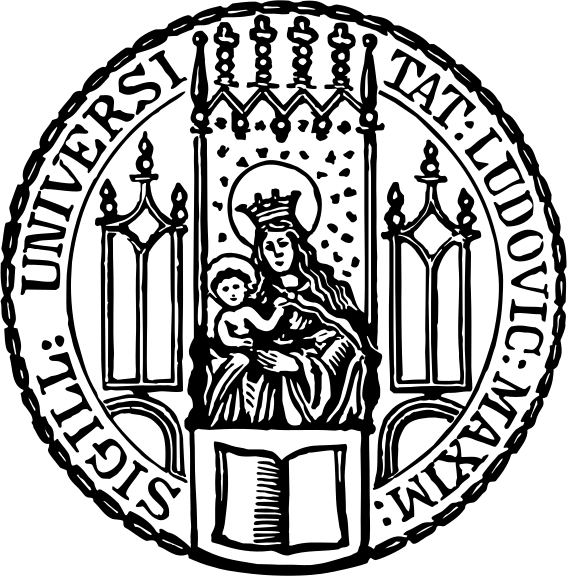
\includegraphics[width=.5\pagewidth]{\mediadir{image/emblem.pdf}}

    \usekomafont{subtitle}
    \@subtitle

    \vspace{.8em}
    \usekomafont{author}
    \@author

    \usekomafont{date}
    \@date

    \vspace{.8em}
    \usekomafont{publishers}
    \@publishers
  \end{center}
\end{titlepage}
\makeatother

\makeatletter
\begin{titlepage}
  \begin{otherlanguage}{ngerman}
    \begin{center}
      \usekomafont{subject}
      Mehrteilchen Quantenoptik

      \vspace{.8em}
      \usekomafont{title}\huge
      Hochpräzise zeitgemittelte optische Potentiale für ultrakalte Atome

      \vspace{.5em}
      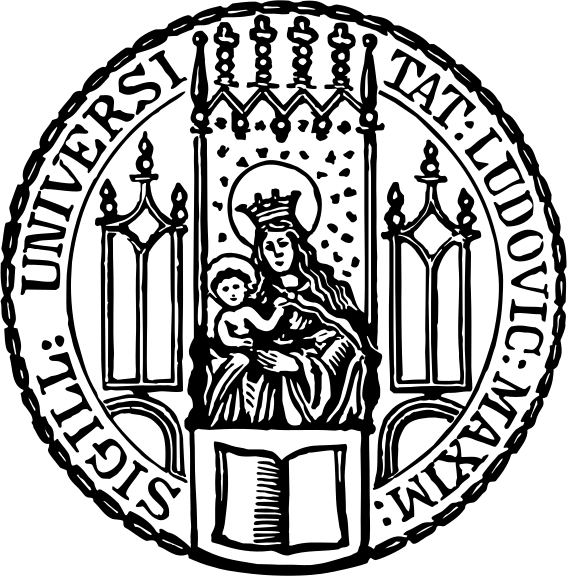
\includegraphics[width=.5\pagewidth]{\mediadir{image/emblem.pdf}}

      \usekomafont{subtitle}
      Bachelorarbeit von

      \vspace{.8em}
      \usekomafont{author}
      \@author

      \usekomafont{date}
      \@date

      \vspace{.8em}
      \usekomafont{publishers}
      entstanden unter der Betreuung von Prof. Dr. Immanuel Block,\\
      Dr. Monika Aidelsburger und Christian Schweitzer.
    \end{center}
  \end{otherlanguage}
\end{titlepage}
\makeatother

\begin{abstract}
Ultracold atoms in optical lattices open up a wide range of possibilities
to simulate many-body quantum phenomena, which would elsewise be neither
computationally nor experimentally tangible.

The topology of the optical lattice is a decisive property of these kind
of experiments and therefore of major interest. Recently, efforts have been
reported to create novel optical potentials through the use of digital
micromirror arrays that permit alterations of localized potentials. Though
promising results have been achieved --- in particular for static potentials
--- limitations due to the mechanical nature of these mirror arrays arise,
for instance, with regard to dynamical control.

In the present work we present an alternative implementation of localized
optical lattice potentials based on acousto-optic deflectors and
direct digital synthesizers.

We will give a brief theoretical introduction into the main concepts, i.e.\
the interaction of neutral atoms with optical potentials as well as the
general operation of direct digital synthesizer and acousto-optic deflectors.
From the physics we can derive the requirements imposed on the technical
implementation of the \gls{rf} signal source and the deflection.

We will find that even though the platform of digital signal synthesis
generally suites our application in terms of modulation capabilities and
resolution, the particular implementation of the \gls{ad9910} demonstrates
several shortcomings.

In the second part we characterize the deflection efficiency of the
acousto-optic deflectors. Towards the end we try to minimize the variance of
the deflection efficiency by performing a random search on the amplitude
segments of the \gls{rf} signal. It turns out that the deflection efficiency
is a highly non-linear function of the applied \gls{rf} power and frequency.
Furthermore minimization of the deflection efficiency variances proves to be
very unstable. Though we can largely preclude electronic defects to be the
source of this behaviour, further investigation is required.
\end{abstract}

\addchap{Acknowledgement}

The success and final outcome of the present work required a lot of guidance
and assistance from many people. Without them it would not have been possible
for me to deliver this work and remember the exciting time I had in the past
weeks.

At most I want to thank my parents for their support, that I have been
privileged to benefit from all the years. Though my life involved many
unexpected turnarounds, I never felt left alone and could rely on your
diverse experience whenever the situation required it.

Further I want to thank Prof. Immanuel Bloch and Dr. Monika Aidelsburger for
creating and sustaining a fertile scientific environment. It has been a
refreshing novelty for me to have the opportunity to have inspiring
discussions at almost any time and to seamlessly implement new ideas without
being limited by the present material.

Equally I want to express my gratitude to all personal involved in the
formation process of my thesis. Especially I want to name Christian Schweizer
with whom it had been a great pleasure to work with. Further I want to thank
Till Klostermann for instantly sharing his deep insights in many problems I
have encountered and his help with the optical setup. Hendrik von Raven I want
to thank for his overall guidance with regard to the electronic equipment.
In addition I owe special thanks to Michael Schreiber who helped me understand
the theoretical foundations of atoms in optical lattices, David Wei for his
hospitality and productive discussions about the acousto-optic deflectors,
and of course biggest thanks to Bodo Hecker for his advice as electrical
engineer and distinct perspective on undergone challenges.

Finally I want to express my gratitude to my friend Dr. Abdullah Sarani for
his suggestions and advice on the final draft.

\addchap{Declearation of Authorship}

\addsec{Statutory Declearation}

I hereby declare that this thesis has been composed solely by myself except
where indicated otherwise by reference or acknowledgment.

The work presented has not been submitted, in whole or in part, in any
previous application for a degree.

\vspace{1em}
\textbf{Munich, \today}


\tableofcontents

\chapter{Introduction}

Many quantum systems studied in condensed matter physics are experimentally
challenging to access as any interactions can destroy the carefully prepared
quantum states. As way forward, experiments with ultracold atoms in
optical lattices give us a highly contorllable environment, giving us the
opportunity to simulate and explore quantum effects and expand our current
understanding of quantum mechanics and statistical physics \cite{Gross2017}.

The central idea behind these types of experiments is to cool down neutral
atoms to micro Kelvin and below, and load them into an optical lattice. At
these temperatures atoms demonstrate quantum behaviour. The optical lattices
act as periodic potentials analogue to the periodic potential found inside
solid state crystal lattices \cite{Lewenstein2007}. Unlike to i.e. real solids
where we have limited prospects to amend a systems properties, lasers driven
by state of the art optics and electronics give us a wide range of well
controllable parameters.

\begin{figure}[h]
  \centering
  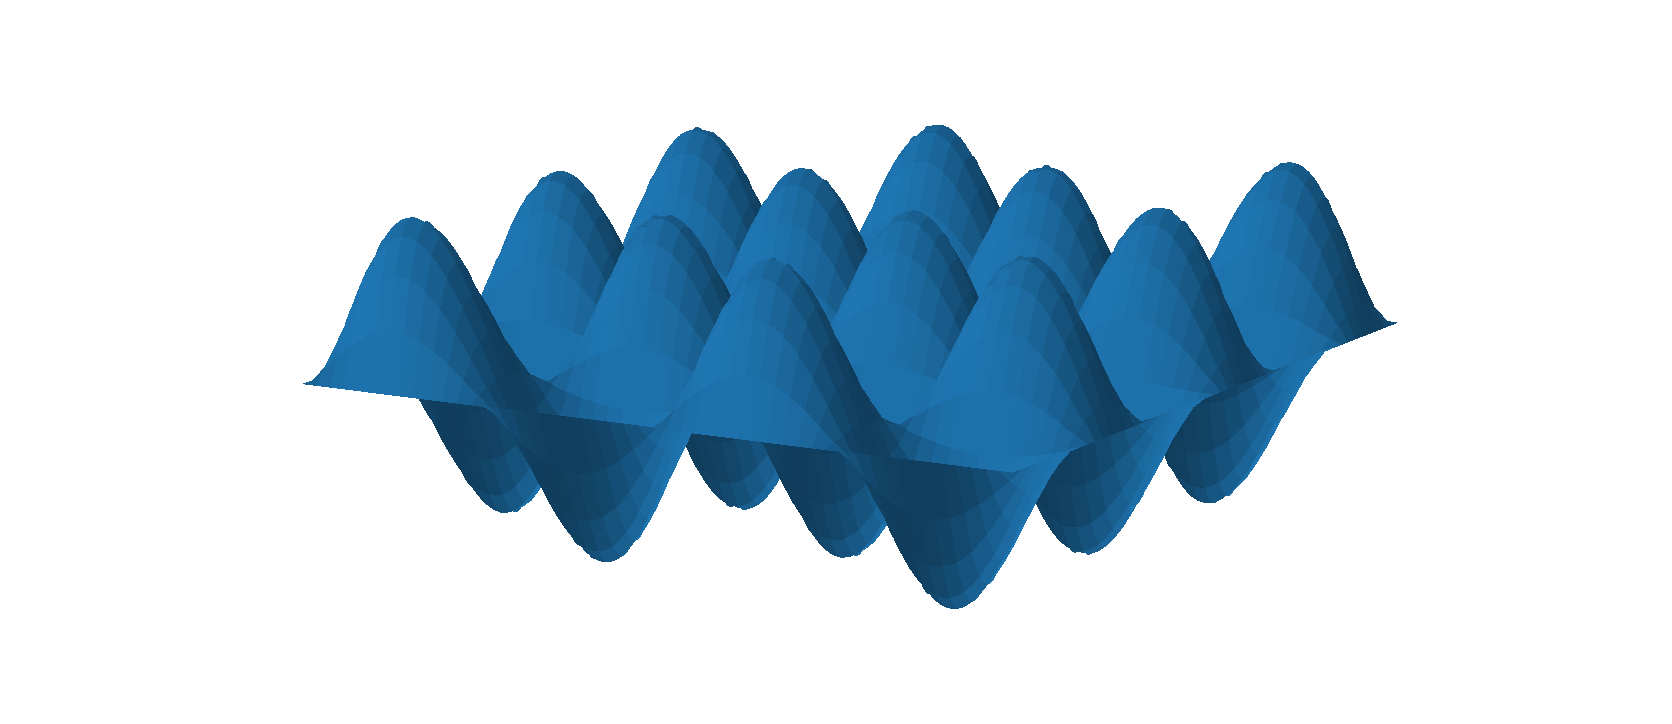
\includegraphics[width=.8\textwidth]{images/optlat/default.pdf}
  \captionsetup{width=.8\textwidth}
  \caption{Periodic potential of a 2D optical lattice. If the kinetic energy
  of the atoms is below the potential energy of the lattice, the atoms will
  locate around the potential minimas.}
  \label{fig:optlat}
\end{figure}

One of the parameters of interest is the ability to apply local potentials
to the system, that can be used to, among others, study lattice inpurities
or quantum interactions. In this work we will present and characterize one
possible implementation of such a local potential generating apparatus.

\section{Related Work}

Local manipulations of atoms inside optical lattices have been known for some
time in the embodiment of optical tweezers that allow trapping, stacking and
sorting of particles \cite{Tadmor2004}. Yet, only recently attempts to
interact with local particle clusters through high-precision time-averaged
optical potentials have been reported \cite{Roy2016}.

In the following we continue on the laid out work \cite{Hertlein2017} which
provided us with an optical setup for single-site manipulation using
\gls{aod} as well as considerations with regard to aperture limited
gaussian beam propagation.

\chapter{Optical lattices}

In the introduction we presented the concept of our envisaged potential
creation. In the following chapter we want to recapitulate the theoretical
foundations of optical lattices and quantum states theoreof. Finally we want
to derive an expression for the quantum tunnelling frequency in order to
estimate the time magnitude in which our apparatus has to operate.

\section{Atom-light interaction}

At first we need to ask ourselves how the laser field propagates as
perturbation potential to the Hamiltonian of the atomic system and how we can
express said potential by physical quantities we control in the experiment.

\subsection{Hamiltonian and dipole approximation}

The Hamiltonian of an electron in an external electromagnetic field reads
\begin{equation}
  \hat{H}_\text{em}
  =\frac{1}{2m}\left(\hat{\vb{p}}+e\vb{A}\right)^2-e\Phi+\hat{V}_0
  \label{eq:hamiltonian_em}
\end{equation}
with vector $\vb{A}$ and scalar potential $\Phi$ of the external field and
the Coulomb potential of the nucleus $\hat{V}_0$. \Cref{eq:hamiltonian_em} is
exact for the hydrogen atom and approximate for alkali atoms with one outer
electron.

Gauge freedom of the vector and scalar potential permits transformations of
type
\begin{align}
  \vb{A}\to\vb{A}+\grad{\chi}
  &&
  \Phi\to\Phi-\pdv{\chi}{t}
\end{align}
with gauge function $\chi(\vb{x},t)$. In the following we choose the gauge
function $\chi=-\vb{A}\cdot\vb{x}$ and assume the dipole approximation
$\vb{A}(\vb{x},t)\approx\vb{A}(t)$. The dipole approximation is reasonable as
wave length of visible light are much larger then atomic length scales
\cite{Gerry2004}. In the dipole approximation $\chi$ satisfies the Coulomb
gauge condition $\divergence{\vb{A}}=0$ allowing us to set $\Phi=0$ as no
external sources are present \cite{Jackson2005}. Finally we can rewrite
\cref{eq:hamiltonian_em} as
\begin{equation}
  \hat{H}_\text{dip}
  =\frac{\hat{\vb{p}}^2}{2m}+\hat{V}_0-\hat{\vb{d}}\cdot\vb{E}
  =\hat{H}_0+\hat{V}_\text{dip}
  \label{eq:hamiltonian_dip}
\end{equation}
with the dipole operator $\hat{\vb{d}}=-e\vb{x}$ and spatially homogeneous
light field $\vb{E}(t)$.

\subsection{Field of an optical lattice}

An one dimensional optical lattices can be generated through the interference
of two counter-propagating Gaussian beams, creating a standing wave
interference pattern. The electrical field component in such a case is given
by
\begin{equation}
  \vb{E}(t)
  =\vb{E}_0\cos(kz)\cos(\omega t)\exp(-\frac{2r^2}{w(z)^2})
  \label{eq:1d_lattice_efield_exact},
\end{equation}
wherein $r$ denotes the beam radius, $w(z)$ the spot size parameter and $k$
the angular wavenumber of the laser. The wavenumber relates to the laser
wavelength via $k=2\pi/\lambda$. The magnetic field component is chosen
in such a way that it satisfies the Maxwell equations but will not be
considered relevant any further as the electron only has a small magnetic
dipole. Analogue to \cite{Rom2009} we will now assume $w(z)\gg r$ and drop
the exponential term in \cref{eq:1d_lattice_efield_exact}, thus simplifying
\cref{eq:1d_lattice_efield_exact} to
\begin{equation}
  \vb{E}(t)
  \approx\vb{E}_0\cos(kz)\cos(\omega t)
  \label{eq:1d_lattice_efield_approx}.
\end{equation}
Note that even the electric field in \cref{eq:1d_lattice_efield_approx} has
a spatial dependency, the dipole approximation still holds in the atomic
reference frame.

\subsection{Effective dipole potential}

We are now going to solve \cref{eq:hamiltonian_dip} for the case of an
electric field of the form \cref{eq:1d_lattice_efield_approx} with
for-off-resonant laser wavelength $\lambda$ and finally derive an expression
for the effective dipole potential.

At $t<0$ the system is in the energy eigenstate $\ket{n}$ of the unperturbated
Hamiltonian
\begin{equation}
  \hat{H}_0\ket{n}
  =E_n\ket{n}
  =\hbar\omega_n\ket{n}
  \label{eq:eigenvalue_energy_unperturbated}.
\end{equation}
At $t>0$ the external light field appears instantaneous. The new state
$\ket{\psi}$ can be expanded in the complete base of the previous energy
eigenstates
\begin{equation}
  \ket{\psi}
  =\sum_nc_n(t)e^{-i\omega_nt}\ket{n}
  \label{eq:state_expansion_unperturbated}.
\end{equation}
Inserting \cref{eq:state_expansion_unperturbated} into the time-dependent
Schrödinger equation with dipole Hamiltonian \cref{eq:hamiltonian_dip} and
applying $\bra{m}e^{i\omega_mt}$ to the right hand side leads us to a set
of differential equations
\begin{equation}
  \dot{c}_m
  =-\frac{i}{\hbar}\sum_nc_n(t)e^{-i\omega_{nm}t}\bra{m}\hat{V}_\text{dip}\ket{n}
  \label{eq:differential_equation_population_dynamics}
\end{equation}
with $\omega_{nm}=\omega_n-\omega_m$, that describe the dynamics of the
probablity amplitudes $c_n(t)$. By using the electric field we derived in
\cref{eq:1d_lattice_efield_approx} we can rewrite the dipole transition
matrix elements
\begin{equation}
  \bra{m}\hat{V}_\text{dip}\ket{n}
  =\hbar\Omega_{nm}\cos(kz)\cos(\omega t)
  \label{eq:elements_dipole_transition_matrix}
\end{equation}
where we introduced the Rabi frequency
$\Omega_{nm}=\bra{n}\hat{\vb{d}}\cdot\vb{E}_0\ket{m}/\hbar$. Explicit values
for general dipole transition elements for one and two electron systems can
be found in \cite{Bethe1957}. Als the transition elements vanishes for states
with same parity, in particular do we have $\Omega_{nn}=0$
\cite{Bartelmann2018}.

\subsubsection{Two state system}

From now on we assume a two state system that initially is only populated in
the ground state $c_g(0)=1,c_e(0)=0$ and the dynamics in
\cref{eq:differential_equation_population_dynamics} are simply described by
\begin{align}
  i\dot{c}_g=\Omega_0c_e(t)\cos(kz)\cos(\omega t)e^{+i\omega_0 t} &&
  i\dot{c}_e=\Omega_0c_g(t)\cos(kz)\cos(\omega t)e^{-i\omega_0 t}
  \label{eq:differential_equation_population_dynamics_two_state_system}.
\end{align}
Expansion of $\cos(\omega t)$ in terms of the exponential function and
dropping $e^{\pm i(\omega+\omega_0)t}$ yields
\begin{align}
  i\dot{c}_g\approx\frac{\Omega_0}{2}c_e(t)\cos(kz)e^{+i\Delta\omega t} &&
  i\dot{c}_e\approx\frac{\Omega_0}{2}c_g(t)\cos(kz)e^{-i\Delta\omega t}
  \label{eq:differential_equation_population_dynamics_two_state_system_rwa}.
\end{align}
The so-called rotating wave approximation is motivated by the fact that
oscillations of frequency $\omega+\omega_0$ are fast compared to changes in
the population dynamics and therefore vanish on average.

We now define $a_g=c_g$ and $a_e=c_ee^{i\Delta\omega t}$ and refine
\cref{eq:differential_equation_population_dynamics_two_state_system_rwa} by
\begin{align}
  i\dot{a}_g=\frac{\Omega_0}{2}a_e(t)\cos(kz) &&
  i\dot{a}_e=\frac{\Omega_0}{2}a_g(t)\cos(kz)-a_e\Delta\omega
  \label{eq:differential_equation_population_dynamics_two_state_system_shift}.
\end{align}
In the former form we can diagonalize the Hamiltonian and find energy
eigenvalues to be
\begin{equation}
  E_{e,g}
  =\frac{\hbar}{2}\left(-\Delta\omega\mp\sqrt{\Omega_0^2+\Delta\omega^2}\right)
  \approx
  =\mp\frac{\hbar\Omega_0^2}{4\Delta\omega}
  \label{eq:eigenvalues_energy_light_shift}
\end{equation}
where we applied Taylor expansion to the square root for
$\Delta\omega\gg\Omega_0$.

In summary atoms in an external off-resonant light field with experience an
effective periodic dipole potential
\begin{equation}
  \hat{V}_\text{eff}
  =V_0\cos^2(kz)
  \qc
  V_0
  =\frac{\hbar\Omega}{4\Delta\omega}\cos^2(kz)
  =\frac{\hbar I_0\cos^2(kz)}{2c_0\epsilon_0\Delta\omega}
  \label{eq:potential_effective}
\end{equation}
with vacuum speed of light $c_0$, dielectric constant $\epsilon_0$ and
maximum intensity $I_0$. Same results can also be obtained by the use of
second order perturbation theory, however the presented approach is more
clear on assumptions and time dependence \cite{Grimm2008}.

\section{Harmonic approximation}

Given the effective lattice potential \cref{eq:potential_effective} the
effective lattice Hamiltonian reads
\begin{equation}
  \hat{H}_\text{eff}
  =\frac{\hat{p}^2}{2m}+\hat{V}_\text{eff}
  \label{eq:hamiltonian_effective}.
\end{equation}
One first naive approach to solve the time-independent Schrödinger equation
subject to the effective lattice Hamiltonian would be to Taylor expand
the effective potential in second order
\begin{equation}
  \hat{V}_\text{eff}
  =V_0\cos^2(kx)
  \approx V_0\left(1-(kx)^2\right)
  \label{eq:potential_harmonic_approximation}
\end{equation}
and give us the Hamiltonian of a linear harmonic quantum oscillator
\begin{equation}
  \hat{H}_\text{har}-V_0
  =\frac{\hat{p}^2}{2m}-V_0k^2x^2
  \label{eq:hamiltonian_harmonic_approximation}
\end{equation}
with well-known energy levels $E_n=\hbar\omega(2n+1)/2$ and frequency
$\omega=\sqrt{V_0/m}k=\sqrt{2V_0E_r}/\hbar$, where we defined the recoil
energy $E_r=(\hbar k)^2/(2m)$ as an atom-independent energy scale.

The harmonic approximation is valid for very deep potentials $V_0\gg E$.
Unfortunately the Gaussian wave functions of the harmonic oscillator decay
fast at the potential boundary such that we have vanishing probability to
find a particle tunneling through the potential.

\section{Periodic lattice potentials}

The following section is dedicated to the quantum mechanics of periodic
lattice potentials. After we revise the formulation of lattice structures,
we will examine Bloch and Wannier states as well as the energy bands arising
in periodic lattice potentials.

\subsection{Lattice structures}

\subsubsection{Bravais lattice}

A Bravais lattice of dimension $N$ consists of the discrete points
\begin{equation}
  \vb{r}
  =\bra{\vb{x}}\ket{\vb{r}}
  =\sum_{i=1}^Nn_i\vb{a}_i
  \qc n_1,\dots,n_N\in\mathbb{Z}
\end{equation}
where $\vb{a}_i$ are the primitive vectors that span the primitive lattice
cell.

\subsubsection{Reciprocal lattice}

We define the reciprocal lattice as the discrete points
\begin{equation}
  \vb{g}
  =\bra{\vb{p}}\ket{\vb{g}}
  =\sum_{i=1}^Nm_i\vb{b}_i
  \qc m_1,\dots,m_N\in\mathbb{Z}
\end{equation}
that satisfy the condition $\exp(\vb{r}\cdot\vb{g})=1$. For a simple cubic
lattice structure $\vb{b}_i=2\pi\vb{a}/{{\vb{a}_i}^2}$ satisfies said
condition. For the subsequent sections we will only consider the one
dimensional simple cubic lattice. Cubic lattices of higher dimension however
can be easily obtained by superposition of the potentials.

\subsubsection{Transformation to reciprocal lattice}

As the reciprocal lattice space can be seen as the Fourier transform of the
Bravais lattice, it is especially simple to express periodic functions and it
suggests the representation of periodic potentials in reciprocal lattice
space. Let $\ket{g_n}$ denote the $n$th reciprocal lattice point then the
transformation rule is
\begin{equation}
  \bra{g_n}\hat{V}\ket{g_m}
  =\int\dd{x}\bra{g_n}\ket{x}^*V(x)\bra{g_m}\ket{x}
  =\int\dd{x}V(x)e^{2ikx(n-m)}
  \label{eq:potential_in_reciprocal_lattice}.
\end{equation}
Evaluation of \cref{eq:potential_in_reciprocal_lattice} for a specific
potential will usually yield a finite number of terms in dependence of
$n-m$ as we actually determine the Fourier coefficients of a discrete Fourier
transform.

\subsection{Bloch states}

Bloch's theorem states that for a periodic lattice potential
\begin{equation}
  V_\text{lat}(\vb{x}+\vb{a})=V_\text{lat}(\vb{x})
  \label{eq:potential_periodic}
\end{equation}
there exists a complete set of wavefunctions that are energy eigenstates
of the Hamiltonian
\begin{equation}
  \hat{H}_\text{lat}
  =\frac{\hat{\vb{p}}^2}{2m}+\hat{V}_\text{lat}
  \label{eq:hamiltonian_periodic},
\end{equation}
and each of these Bloch waves can be written into the form
\begin{equation}
  \bra{\vb{x}}\ket{\Psi^n_{\vb{q}}}
  =\Psi^n_{\vb{q}}(\vb{x})
  =e^{i\vb{q}\cdot\vb{x}}\psi^n_{\vb{q}}(\vb{x})
  \label{eq:state_bloch}
\end{equation}
with $\psi^n_{\vb{q}}(\vb{x}+\vb{a})=\psi^n_{\vb{q}}(\vb{x})$, wave vector
$\vb{q}$ and bandindex $n$. We confine the wave number to the first Brillouin
zone $-k<q<+k$. For a proof of Bloch's theorem see \cite{Roessler2004} or
\cite{Bartelmann2018}.

\subsection{Energy bands}

The Bloch states \cref{eq:state_bloch} can be used as ansatz to solve the
periodic lattice Hamiltonian
\begin{equation}
  \hat{H}_\text{lat}
  =\frac{\hat{p}^2}{2m}+\hat{V}_\text{lat}
  \label{eq:hamiltonian_lattice}.
\end{equation}
We notice that by the product rule
$\hat{p}^2\Psi^n_q(x)=e^{iqx}(\hat{p}+\hbar q)\psi^n_q(x)$,
thus we find
\begin{equation}
  E^n_q\ket{\Psi^n_{q}}
  =\hat{H}_{lat}\ket{\Psi^n_{q}}
  =e^{iqx}\left(\frac{(\hat{p}+\hbar q)^2}{2m}+\hat{V}_\text{lat}\right)\ket{\psi^n_{q}}
  \label{eq:eigenvalue_energy_lattice}.
\end{equation}
Expansion of the state $\ket{n,q}$ in states of the reciprocal lattice returns
\begin{equation}
  \ket{\Psi^n_q}
  =\left(\sum_s\ket{g_s}\bra{g_s}\right)\ket{\Psi^n_q}
  =\sum_s\braket{g_s}{\Psi^n_q}\ket{g_s}
  =\sum_sc^n_{sq}\ket{g_s}
  \label{eq:state_bloch_in_reciprocal_lattice}.
\end{equation}
The momentum eigenvalues of the state $\ket{g_s}$ can be found by expansion
into position space
\begin{equation}
  \hat{p}\ket{g_s}
  =\int\int\dd{x}\dd{y}\ket{y}\bra{y}\hat{p}\ket{x}\bra{x}\ket{g_s}
  \label{eq:eigenvalue_momentum_reciprocal_lattice1}.
\end{equation}
With $\bra{y}\hat{p}\ket{x}=-i\hbar\delta(y-x)\dv{x}$ we can take the
derivative of $\bra{x}\ket{g_s}=e^{2ikxs}$ and simplify
\cref{eq:eigenvalue_momentum_reciprocal_lattice1} down to
\begin{equation}
  \hat{p}\ket{g_s}
  =2\hbar ks\int\dd{x}\ket{x}\bra{x}\ket{g_s}
  =2\hbar ks\ket{g_s}
  \label{eq:eigenvalue_momentum_reciprocal_lattice2}.
\end{equation}
Finally we insert \cref{eq:state_bloch_in_reciprocal_lattice} into
\cref{eq:eigenvalue_energy_lattice} and apply $\bra{g_t}$ to the
right hand side while using \cref{eq:potential_in_reciprocal_lattice} and
\cref{eq:eigenvalue_momentum_reciprocal_lattice2}, yielding
\begin{equation}
  E^n_qc^n_{tq}
  =c^n_{tq}\frac{(2s+q/k)^2}{2m}E_r+\sum_sc^n_{sq}\bra{g_t}\hat{V}_\text{lat}\ket{g_s}
  \label{eq:eigenvalue_energy_lattice_explicit}
\end{equation}
with recoil energy $E_r=\hbar^2k^2/(2m)$.
\Cref{eq:eigenvalue_energy_lattice_explicit} has to be solved for known
$\hat{V}_\text{lat}$ numerically. We will do this later for the effective
optical lattice potential from \cref{eq:potential_effective}.

\subsection{Wannier states}

So far we studied the effects of a periodic lattice potential on the energy
levels and the Bloch wave functions that propagate over the complete lattice.
Lattice hopping however is a local effect, therefore we need a spatially
localized set of wave functions to describe the effect of lattice hopping.
Fortunately the so called Wannier fullfill these requirements.

\subsubsection{Definition via Bloch superpositions}

The orthodox definition of the Wannier function with bandindex $n$ at lattice
site $l$ reads
\begin{equation}
  \ket{\phi^n_{l}}
  =\frac{1}{\sqrt{N}}\sum_qe^{-iqla}\ket{\Psi^n_{q}}
  \label{eq:state_wannier_orthodox}
\end{equation}
wherein $\ket{\Psi^n_q}$ is the Bloch wave functions from
\cref{eq:state_bloch}, $N$ the total number of lattice sites and the sum
over $q$ is confined to the first Brillouin zone with $q$ that satisfy the
periodic boundary condition $-k<q=2ki/N<+k$ with integer $i\in\mathbb{Z}$.

\subsubsection{Definition via the band projected position operator}

The defintion \cref{eq:state_wannier_orthodox} is valid for simple lattice
structures, however for more sophisticated lattices Gauge freedom of the
phase of the Bloch states leads to different Wannier states, whereof only
one is the maximally localized one \cite{Goerg2014}. One can find the
phase of the Bloch state that is maximally localized by minimizing the spread
of the Wannier states, however there also exists a more general definition
that incorporates the phase ubiquity. In the general definition the Wannier
states are best to construct as the eigenstates of the band projected
position operator. The band projector to bandindex $n$ is defined as
\begin{equation}
  \hat{P}_n
  =\sum_q\ket{\Psi^n_q}\bra{\Psi^n_q}
  \label{eq:operator_band_projector}
\end{equation}
and the band projected position operator just follows as
\begin{equation}
  \hat{x}_n
  =\hat{P}_n\hat{x}_n\hat{P}_n
  \label{eq:operator_band_projected_position}.
\end{equation}
The wannier states are now defined as the eigenstates of the eigenvalue
equation
\begin{equation}
  \hat{x}_n\ket{\phi^n_l}=x^n_l\ket{\phi^n_l}
  \label{eq:eigenvalue_band_projected_position}
\end{equation}
where $x^n_l$ is the $l$th lattice site in the $n$th energy band. Choosing
the Bloch base to find the elements of the band projected position operator
\cref{eq:operator_band_projected_position} through
\begin{equation}
  X^{nn^\prime}_{qq^\prime}
  =\bra{\Psi^n_q}\hat{x}_n\ket{\Psi^{n^\prime}_{q^\prime}}
  =\int_0^{Na}\dd{x}\Psi^n_q(x)^*x\Psi^{n^\prime}_{q^\prime}(x)
  \label{eq:element_band_projected_position}
\end{equation}
which give an analytical expression to solve to determine the matrix elements
\cite{Bissbort2013}. Let $d^{mn}_{lq}$ be the diagonalized
matrix $X^{nn^\prime}_{qq^\prime}$ in
\cref{eq:element_band_projected_position} then the Wannier states are fully
determined by
\begin{equation}
  \ket{\phi^n_l}
  =\sum_{n,q}d^{mn}_{lq}\ket{\Phi^n_q}
  \label{eq:state_wannier}.
\end{equation}

\subsection{Hopping amplitude}

With the previous tools in place we are now set to give an expression for the
quantum hopping amplitude between lattices.

We define the hopping probability from lattice site $l$ to lattice site
$l^\prime$ at bandindex $n$ as
\begin{equation}
  J^n_{ll^\prime}
  =-\bra{\phi^n_l}\hat{H}_\text{lat}\ket{\phi^n_{l^\prime}}
  \label{eq:element_hopping}
\end{equation}
this definition makes intuitive sense if we remind us at the dipole transition
element and the Wannier states. Using the orthodox definition of the Wannier
states \cref{eq:state_wannier_orthodox} for \cref{eq:element_hopping} we find
\begin{equation}
  J^n_{ll^\prime}
  =\frac{1}{N}\sum_{q,q^\prime}e^{iqa(l-l^\prime)}
  \bra{\Psi^n_q}\hat{H}_\text{lat}\ket{\Psi^n_{q^\prime}}
  \label{eq:element_hopping2}.
\end{equation}
The Bloch states are energy eigenstates
\cref{eq:eigenvalue_energy_lattice_explicit} and orthonormal, henceforth
\begin{equation}
  J^n_{ll^\prime}
  =\frac{1}{N}\sum_{q}E^n_qe^{iqa(l-l^\prime)}
  \label{eq:element_hopping3}.
\end{equation}
Expression \cref{eq:element_hopping3} is exact for a given number of lattices
$N$ and can be evaluated numerically. The form of \cref{eq:element_hopping3}
resembles a discrete Fourier transform. The inverse Fourier transform gives us
the energies in terms of the hopping probabilites
\begin{equation}
  E^n_q
  =\sum_{l-l^\prime}J^n_{l,l^\prime}e^{-iqa(l-l^\prime)}
  \label{eq:element_energy_hopping}
\end{equation}
which in practice is easier to calculate then \cref{eq:element_hopping} as
can be seen in the consecutive section.

\subsubsection{Tight-binding approximation}

For deep potentials $V_0\gtrapprox3E_r$ hopping only contributes from direct
neighbour sites \cite{Rom2009}. Thus we can \cref{eq:element_energy_hopping}
reduces to
\begin{equation}
  E^n_q
  \approx J^n_{l,l+1}e^{-iqa}+J^n_{l,l-1}e^{+iqa}+J^n_{ll}
  =J^n_0+2J^n_1\cos(qa)
  \label{eq:element_energy_hopping_tb_approx}
\end{equation}
where we have $J^n_{l,l-1}=J^n_{l,l+1}=J_1$ because of translation invariance.
Using evaluation of $J^n_0=J^n_{ll}$ with \cref{eq:element_hopping} tells us
that $J^n_0$ just is the average energy of an energy band. Evaluation of
\cref{eq:element_energy_hopping_tb_approx} at $q=0$ and $q=k$ and subtracting
the results from another yields us
\begin{equation}
  J^n_1\approx\frac{1}{4}\left(E^n_k-E^n_0\right)
  \label{eq:hopping_amplitude_energies}
\end{equation}
which says that the hopping probability is approximate one quarter of the
energy bandwidth.

\section{Computation of hopping frequency}

Finally we want to apply the previous results on the previously found
effective potential $V(z)=V_0\cos^2(kz)$ \cref{eq:potential_effective}. Using
\cref{eq:potential_in_reciprocal_lattice} we find that the matrix elements of
the effective potential indeed have the simple form
\begin{equation}
  \bra{g_s}\hat{V}_\text{eff}\ket{g_t}
  =\frac{1}{4}V_0\left(2\delta^s_t+\delta^s_{t-1}+\delta^s_{t+1}\right)
  \label{eq:elements_effective_potential_in_reciprocal_state}
\end{equation}
in reciprocal space. Using
\cref{eq:elements_effective_potential_in_reciprocal_state} for the matrix
elements of the effective Hamiltonian using
\cref{eq:eigenvalue_energy_lattice_explicit} gives us
\begin{equation}
  \bra{g_s}\hat{H}_\text{eff}\ket{g_t}
  =\begin{cases}
    (s+q/k)^2E_r+\frac{1}{2}V_0, & \text{if }s=t\\
    \frac{1}{4}V_0, & \text{if } \abs{s-t}=1\\
    0, & \text{otherwise}
  \end{cases}.
\end{equation}
Back at \cref{eq:eigenvalue_energy_lattice_explicit} we are set to determine
the coefficients of the Bloch states
\cref{eq:state_bloch_in_reciprocal_lattice} numerically and thereof the
hopping terms using either the exact expression
\cref{eq:element_energy_hopping} over all quasi-momenta $\hbar q$ or through
the tight binding approximation \cref{eq:hopping_amplitude_energies}.

\subsection{Analytical proximity}

The literature \cite{Bloch2008} also reports the analytical proxmity
\begin{equation}
  J^n_1\approx
  \frac{4}{\sqrt{\pi}}\left(\frac{V_0}{E_r}\right)^{3/4}\exp(-2\sqrt{V_0/E_r})
  \label{eq:hopping_proximity}
\end{equation}
to be valid for sinusoidal potentials like \cref{eq:potential_effective} and
to be derived from the Mathieu equation. The Mathieu equation can be obtained
from the time-independent Schrödinger equation with
$V_0\cos^2(kx)=\frac{1}{2}V_0\left(1-\cos(2kx)\right)$. \cite{Connor1984}
gives a more elaborate deviation of \cref{eq:hopping_proximity}.

\subsection{Results}

Comparison of different methods to obtain the hopping amplitude and how
they behave for different potential deeps. Conversion of the hopping term to
a frequency and significance for our experiment.

\chapter{Hopping frequency}

In the previous chapter we focused on the effective potential obtained by the
superposition of the averaged superposition of the perturbation potential and
the lattice potential. In this chapter we want to emphasize on the physics
that determine the time scale of the perturbation potential.

\section{Harmonic approximation}

Given the effective lattice potential \cref{eq:potential_effective} the
effective lattice Hamiltonian reads
\begin{equation}
  \hat{H}_\text{eff}
  =\frac{\hat{p}^2}{2m}+\hat{V}_\text{eff}
  \label{eq:hamiltonian_effective}.
\end{equation}
One first naive approach to solve the time-independent Schrödinger equation
subject to the effective lattice Hamiltonian would be to Taylor expand
the effective potential in second order
\begin{equation}
  \hat{V}_\text{eff}
  =V_0\cos^2(kx)
  \approx V_0\left(1-\frac{1}{2}(kx)^2\right)
  \label{eq:potential_harmonic_approximation}.
\end{equation}
With \cref{eq:potential_harmonic_approximation} we get the Hamiltonian of a
linear harmonic quantum oscillator
\begin{equation}
  \hat{H}_\text{har}-V_0
  =\frac{\hat{p}^2}{2m}-\frac{1}{2}V_0k^2x^2
  \label{eq:hamiltonian_harmonic_approximation}
\end{equation}
with well-known energy levels
\begin{equation}
  E_n=\hbar\omega(2n+1)/2
  \qc
  \omega=\sqrt{\abs{V_0}/m}k=\sqrt{2\abs{V_0}E_r}/\hbar
  \label{eq:energy_harmonic_approximation}
\end{equation}
where we introduced the recoil energy $E_r=(\hbar k)^2/(2m)$ as an
atom-independent energy scale. In natural scales of the quantum oscillator
we find the time independent wave functions for energy level $n$ to be
\begin{equation}
  \psi_n(x)
  =
  \bra{x}\ket{\psi}
  =
  \frac{\exp(-\frac{1}{2}x^2)}{\sqrt{2^nn!}\pi^{1/4}}H_n(x)
  \label{eq:wavefunction_harmonic}
\end{equation}
where $H_n(x)$ is the $n$th Hermite polynom and the spatial dimension is
expessed in units of $(2E_r/\abs{V_0})^{1/4}/k$.

In \Cref{fig:wavefunction_harmonic} we have visualized the harmonic
approximation for lattice depths $V_0=-50E_r$ including the probability
densities of the wave functions up to the fourth energy level.

\begin{figure}[ht]
  \centering
  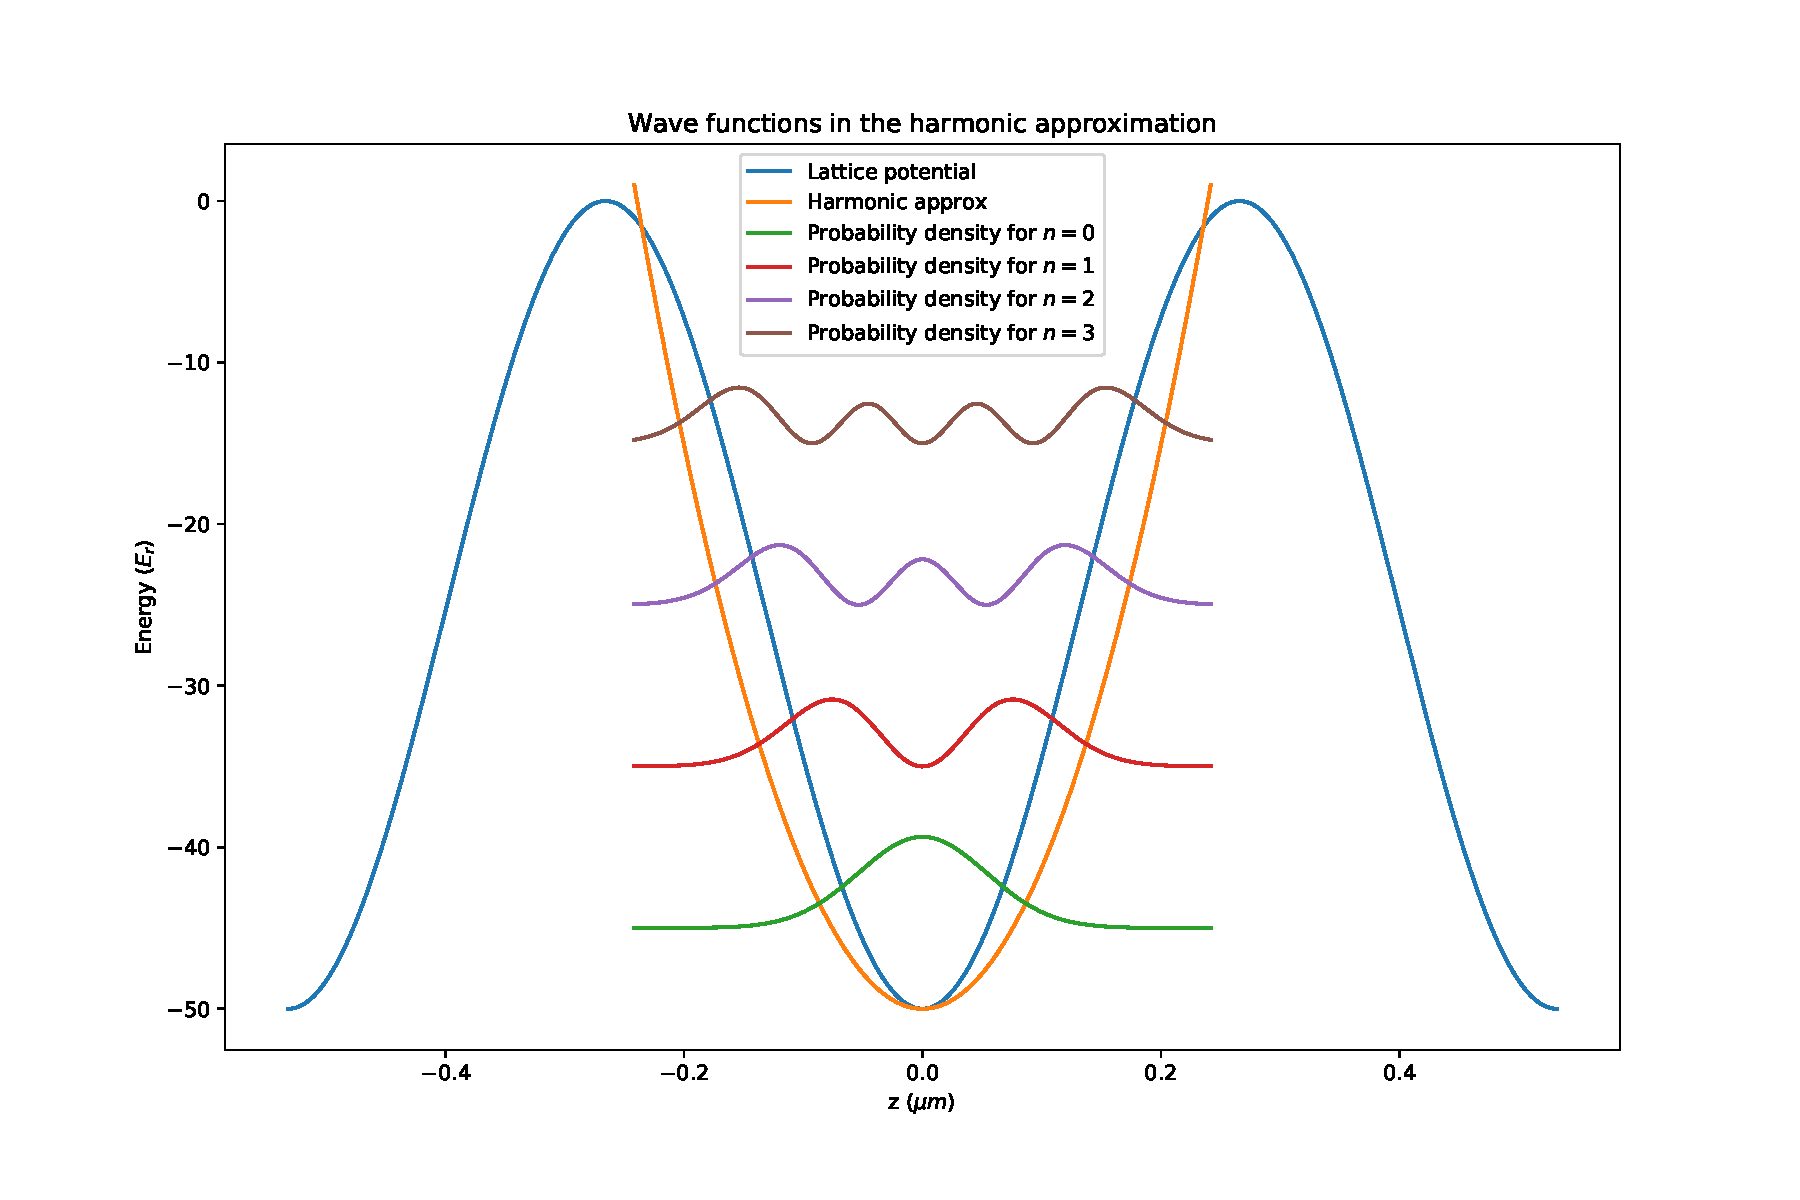
\includegraphics[width=\textwidth]{\figuredir{hopping/harmonic.pdf}}
  \captionsetup{width=.9\textwidth}
  \caption{Harmonic approximation of the optical lattice potential with
    probability density of harmonic wave functions. We can see that the
    probability density decays exponentially at the potential boundaries
    such that the probability for an atom to tunnel to the neighbouring
    lattice site vanish.
  }
  \label{fig:wavefunction_harmonic}
\end{figure}

We can see that the probablity density decays exponentially at the potential
boundary and thereby the probability for a particle to tunnel through the
lattice potential vanishes. We conclude that the harmonic approximation is
not suited to describe the hopping probability and we proceed with a more
elaborate treatment of \cref{eq:hamiltonian_effective} in the next section.

\section{Periodic lattice potentials}

The following section is dedicated to the quantum mechanics of periodic
lattice potentials. We will develope a toolset which allows us to find an
exact solution to \cref{eq:hamiltonian_effective} and other periodic
potentials. We are going to start of with a recap of lattice structures and
examine how Bloch states can be used as ansatz for periodic potentials. From
there on we will derive a general expression for the energy band structure
that arises with Bloch states and then finally discuss Wannier states as
a change of reference frame from the expanded lattice structure to the local
lattice sites.

\subsection{Lattice structures}

A Bravais lattice of dimension $N$ consists of the discrete points
\begin{equation}
  \vb{r}
  =\bra{\vb{x}}\ket{\vb{r}}
  =\sum_{i=1}^Nn_i\vb{a}_i
  \qc n_1,\dots,n_N\in\mathbb{Z}
\end{equation}
where $\vb{a}_i$ are the primitive vectors that span the primitive lattice
cell. We define the reciprocal lattice as the discrete points
\begin{equation}
  \vb{g}
  =\bra{\vb{p}}\ket{\vb{g}}
  =\sum_{i=1}^Nm_i\vb{b}_i
  \qc m_1,\dots,m_N\in\mathbb{Z}
\end{equation}
that satisfy the condition $\exp(\vb{r}\cdot\vb{g})=1$. For a simple cubic
lattice structure $\vb{b}_i=2\pi\vb{a}/{{\vb{a}_i}^2}$ satisfies said
condition. For the subsequent sections we will only consider the one
dimensional simple cubic lattice. Cubic lattices of higher dimension however
can be easily obtained by superposition of the potentials.

As the reciprocal lattice space can be seen as the Fourier transform of the
Bravais lattice, it is especially simple to express periodic functions and it
suggests the representation of periodic potentials in reciprocal lattice
space. Let $\ket{g_n}$ denote the $n$th reciprocal lattice point then the
transformation rule is
\begin{equation}
  \bra{g_n}\hat{V}\ket{g_m}
  =\int\dd{x}\bra{g_n}\ket{x}^*V(x)\bra{g_m}\ket{x}
  =\int\dd{x}V(x)e^{2ikx(n-m)}
  \label{eq:potential_in_reciprocal_lattice}.
\end{equation}
Evaluation of \cref{eq:potential_in_reciprocal_lattice} for a specific
potential will usually yield a finite number of terms in dependence of
$n-m$ as we actually determine the Fourier coefficients of a discrete Fourier
transform.

\subsection{Bloch states}

Bloch's theorem states that for a periodic lattice potential
\begin{equation}
  V_\text{lat}(\vb{x}+\vb{a})=V_\text{lat}(\vb{x})
  \label{eq:potential_periodic}
\end{equation}
there exists a complete set of wavefunctions that are energy eigenstates
of the Hamiltonian
\begin{equation}
  \hat{H}_\text{lat}
  =\frac{\hat{\vb{p}}^2}{2m}+\hat{V}_\text{lat}
  \label{eq:hamiltonian_periodic},
\end{equation}
and each of these Bloch waves can be written into the form
\begin{equation}
  \bra{\vb{x}}\ket{\Psi^n_{\vb{q}}}
  =\Psi^n_{\vb{q}}(\vb{x})
  =e^{i\vb{q}\cdot\vb{x}}\psi^n_{\vb{q}}(\vb{x})
  \label{eq:state_bloch}
\end{equation}
with $\psi^n_{\vb{q}}(\vb{x}+\vb{a})=\psi^n_{\vb{q}}(\vb{x})$, wave vector
$\vb{q}$ and bandindex $n$. We confine the wave number to the first Brillouin
zone $-k<q<+k$. For a proof of Bloch's theorem see \cite{Roessler2004} or
\cite{Bartelmann2018}.

\subsection{Energy bands}

The Bloch states \cref{eq:state_bloch} can be used as ansatz to solve the
periodic lattice Hamiltonian
\begin{equation}
  \hat{H}_\text{lat}
  =\frac{\hat{p}^2}{2m}+\hat{V}_\text{lat}
  \label{eq:hamiltonian_lattice}.
\end{equation}
We notice that by the product rule
$\hat{p}^2\Psi^n_q(x)=e^{iqx}(\hat{p}+\hbar q)\psi^n_q(x)$,
thus we find
\begin{equation}
  E^n_q\ket{\Psi^n_{q}}
  =\hat{H}_{lat}\ket{\Psi^n_{q}}
  =e^{iqx}\left(\frac{(\hat{p}+\hbar q)^2}{2m}+\hat{V}_\text{lat}\right)\ket{\psi^n_{q}}
  \label{eq:eigenvalue_energy_lattice}.
\end{equation}
Expansion of the state $\ket{n,q}$ in states of the reciprocal lattice returns
\begin{equation}
  \ket{\Psi^n_q}
  =\left(\sum_s\ket{g_s}\bra{g_s}\right)\ket{\Psi^n_q}
  =\sum_s\braket{g_s}{\Psi^n_q}\ket{g_s}
  =\sum_sc^n_{sq}\ket{g_s}
  \label{eq:state_bloch_in_reciprocal_lattice}.
\end{equation}
The momentum eigenvalues of the state $\ket{g_s}$ can be found by expansion
into position space
\begin{equation}
  \hat{p}\ket{g_s}
  =\int\int\dd{x}\dd{y}\ket{y}\bra{y}\hat{p}\ket{x}\bra{x}\ket{g_s}
  \label{eq:eigenvalue_momentum_reciprocal_lattice1}.
\end{equation}
With $\bra{y}\hat{p}\ket{x}=-i\hbar\delta(y-x)\dv{x}$ we can take the
derivative of $\bra{x}\ket{g_s}=e^{2ikxs}$ and simplify
\cref{eq:eigenvalue_momentum_reciprocal_lattice1} down to
\begin{equation}
  \hat{p}\ket{g_s}
  =2\hbar ks\int\dd{x}\ket{x}\bra{x}\ket{g_s}
  =2\hbar ks\ket{g_s}
  \label{eq:eigenvalue_momentum_reciprocal_lattice2}.
\end{equation}
Finally we insert \cref{eq:state_bloch_in_reciprocal_lattice} into
\cref{eq:eigenvalue_energy_lattice} and apply $\bra{g_t}$ to the
right hand side while using \cref{eq:potential_in_reciprocal_lattice} and
\cref{eq:eigenvalue_momentum_reciprocal_lattice2}, yielding
\begin{equation}
  E^n_qc^n_{tq}
  =c^n_{tq}\frac{(2s+q/k)^2}{2m}E_r+\sum_sc^n_{sq}\bra{g_t}\hat{V}_\text{lat}\ket{g_s}
  \label{eq:eigenvalue_energy_lattice_explicit}
\end{equation}
with recoil energy $E_r=\hbar^2k^2/(2m)$.
\Cref{eq:eigenvalue_energy_lattice_explicit} has to be solved for known
$\hat{V}_\text{lat}$ numerically. We will do this later for the effective
optical lattice potential from \cref{eq:potential_effective}.

\subsection{Wannier states}

So far we studied the effects of a periodic lattice potential on the energy
levels and the Bloch wave functions that propagate over the complete lattice.
Lattice hopping however is a local effect, therefore we need a spatially
localized set of wave functions to describe the effect of lattice hopping.
Fortunately the so called Wannier fullfill these requirements.

\subsubsection{Definition via Bloch superpositions}

The orthodox definition of the Wannier function with bandindex $n$ at lattice
site $l$ reads
\begin{equation}
  \ket{\phi^n_{l}}
  =\frac{1}{\sqrt{N}}\sum_qe^{-iqla}\ket{\Psi^n_{q}}
  \label{eq:state_wannier_orthodox}
\end{equation}
wherein $\ket{\Psi^n_q}$ is the Bloch wave functions from
\cref{eq:state_bloch}, $N$ the total number of lattice sites and the sum
over $q$ is confined to the first Brillouin zone with $q$ that satisfy the
periodic boundary condition $-k<q=2ki/N<+k$ with integer $i\in\mathbb{Z}$.

\subsubsection{Definition via the band projected position operator}

The defintion \cref{eq:state_wannier_orthodox} is valid for simple lattice
structures, however for more sophisticated lattices Gauge freedom of the
phase of the Bloch states leads to different Wannier states, whereof only
one is the maximally localized one \cite{Goerg2014}. One can find the
phase of the Bloch state that is maximally localized by minimizing the spread
of the Wannier states, however there also exists a more general definition
that incorporates the phase ubiquity. In the general definition the Wannier
states are best to construct as the eigenstates of the band projected
position operator. The band projector to bandindex $n$ is defined as
\begin{equation}
  \hat{P}_n
  =\sum_q\ket{\Psi^n_q}\bra{\Psi^n_q}
  \label{eq:operator_band_projector}
\end{equation}
and the band projected position operator just follows as
\begin{equation}
  \hat{x}_n
  =\hat{P}_n\hat{x}_n\hat{P}_n
  \label{eq:operator_band_projected_position}.
\end{equation}
The wannier states are now defined as the eigenstates of the eigenvalue
equation
\begin{equation}
  \hat{x}_n\ket{\phi^n_l}=x^n_l\ket{\phi^n_l}
  \label{eq:eigenvalue_band_projected_position}
\end{equation}
where $x^n_l$ is the $l$th lattice site in the $n$th energy band. Choosing
the Bloch base to find the elements of the band projected position operator
\cref{eq:operator_band_projected_position} through
\begin{equation}
  X^{nn^\prime}_{qq^\prime}
  =\bra{\Psi^n_q}\hat{x}_n\ket{\Psi^{n^\prime}_{q^\prime}}
  =\int_0^{Na}\dd{x}\Psi^n_q(x)^*x\Psi^{n^\prime}_{q^\prime}(x)
  \label{eq:element_band_projected_position}
\end{equation}
which give an analytical expression to solve to determine the matrix elements
\cite{Bissbort2013}. Let $d^{mn}_{lq}$ be the diagonalized
matrix $X^{nn^\prime}_{qq^\prime}$ in
\cref{eq:element_band_projected_position} then the Wannier states are fully
determined by
\begin{equation}
  \ket{\phi^n_l}
  =\sum_{n,q}d^{mn}_{lq}\ket{\Phi^n_q}
  \label{eq:state_wannier}.
\end{equation}

\subsection{Hopping amplitude}

With the previous tools in place we are now set to give an expression for the
quantum hopping amplitude between lattices.

We define the hopping probability from lattice site $l$ to lattice site
$l^\prime$ at bandindex $n$ as
\begin{equation}
  J^n_{ll^\prime}
  =-\bra{\phi^n_l}\hat{H}_\text{lat}\ket{\phi^n_{l^\prime}}
  \label{eq:element_hopping}
\end{equation}
this definition makes intuitive sense if we remind us at the dipole transition
element and the Wannier states. Using the orthodox definition of the Wannier
states \cref{eq:state_wannier_orthodox} for \cref{eq:element_hopping} we find
\begin{equation}
  J^n_{ll^\prime}
  =\frac{1}{N}\sum_{q,q^\prime}e^{iqa(l-l^\prime)}
  \bra{\Psi^n_q}\hat{H}_\text{lat}\ket{\Psi^n_{q^\prime}}
  \label{eq:element_hopping2}.
\end{equation}
The Bloch states are energy eigenstates
\cref{eq:eigenvalue_energy_lattice_explicit} and orthonormal, henceforth
\begin{equation}
  J^n_{ll^\prime}
  =\frac{1}{N}\sum_{q}E^n_qe^{iqa(l-l^\prime)}
  \label{eq:element_hopping3}.
\end{equation}
Expression \cref{eq:element_hopping3} is exact for a given number of lattices
$N$ and can be evaluated numerically. The form of \cref{eq:element_hopping3}
resembles a discrete Fourier transform. The inverse Fourier transform gives us
the energies in terms of the hopping probabilites
\begin{equation}
  E^n_q
  =\sum_{l-l^\prime}J^n_{l,l^\prime}e^{-iqa(l-l^\prime)}
  \label{eq:element_energy_hopping}
\end{equation}
which in practice is easier to calculate then \cref{eq:element_hopping} as
can be seen in the consecutive section.

\subsubsection{Tight-binding approximation}

For deep potentials $V_0\gtrapprox3E_r$ hopping only contributes from direct
neighbour sites \cite{Rom2009}. Thus we can \cref{eq:element_energy_hopping}
reduces to
\begin{equation}
  E^n_q
  \approx J^n_{l,l+1}e^{-iqa}+J^n_{l,l-1}e^{+iqa}+J^n_{ll}
  =J^n_0+2J^n_1\cos(qa)
  \label{eq:element_energy_hopping_tb_approx}
\end{equation}
where we have $J^n_{l,l-1}=J^n_{l,l+1}=J_1$ because of translation invariance.
Using evaluation of $J^n_0=J^n_{ll}$ with \cref{eq:element_hopping} tells us
that $J^n_0$ just is the average energy of an energy band. Evaluation of
\cref{eq:element_energy_hopping_tb_approx} at $q=0$ and $q=k$ and subtracting
the results from another yields us
\begin{equation}
  J^n_1\approx\frac{1}{4}\left(E^n_k-E^n_0\right)
  \label{eq:hopping_amplitude_energies}
\end{equation}
which says that the hopping probability is approximate one quarter of the
energy bandwidth.

\section{Numerical determination of hopping frequency}

Finally we want to apply the previous results on the previously found
effective potential $V(z)=V_0\cos^2(kz)$ \cref{eq:potential_effective}. Using
\cref{eq:potential_in_reciprocal_lattice} we find that the matrix elements of
the effective potential indeed have the simple form
\begin{equation}
  \bra{g_s}\hat{V}_\text{eff}\ket{g_t}
  =\frac{1}{4}V_0\left(2\delta^s_t+\delta^s_{t-1}+\delta^s_{t+1}\right)
  \label{eq:elements_effective_potential_in_reciprocal_state}
\end{equation}
in reciprocal space. Using
\cref{eq:elements_effective_potential_in_reciprocal_state} for the matrix
elements of the effective Hamiltonian using
\cref{eq:eigenvalue_energy_lattice_explicit} gives us
\begin{equation}
  H_{st}
  =\bra{g_s}\hat{H}_\text{eff}\ket{g_t}
  =\begin{cases}
    (2s+q/k)^2E_r+\frac{1}{2}V_0, & \text{if }s=t\\
    \frac{1}{4}V_0, & \text{if } \abs{s-t}=1\\
    0, & \text{otherwise}
  \end{cases}
  \label{eq:hamiltonian_effective_elements}.
\end{equation}
Now that we have found a definite expression for the Hamiltonian matrix
elements \cref{eq:hamiltonian_effective_elements} we can use the energy
eigenvalue equation \cref{eq:eigenvalue_energy_lattice_explicit} to calculate
the energy bands in dependence of the quasi-momentum $\hbar q$.

\begin{figure}[ht]
  \centering
  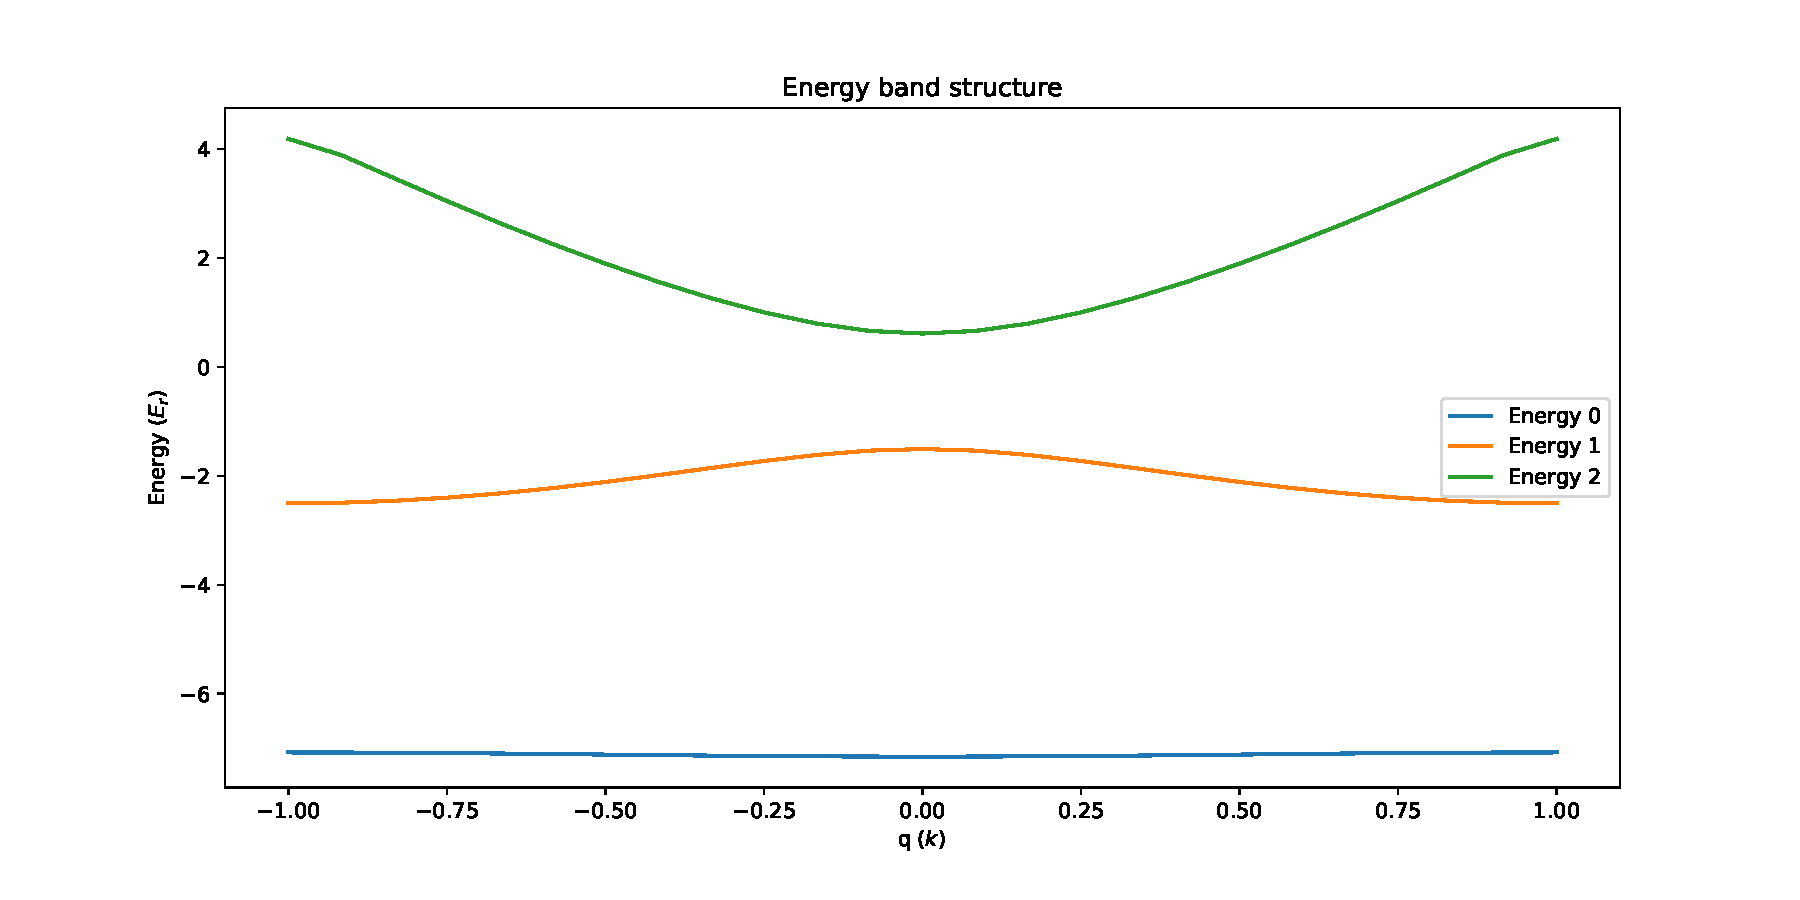
\includegraphics[width=\textwidth]{\figuredir{hopping/band-structure.pdf}}
  \captionsetup{width=.9\textwidth}
  \caption{
    First three energy bands for an optical lattice depth of $V_0=-10E_r$.
  }
  \label{fig:band_structure}
\end{figure}

In \Cref{fig:band_structure} we visualized the first energy bands for a
lattice depth of $V_0=-10E_r$ from a matrix with dimensions 60.

the coefficients of the Bloch states
\cref{eq:state_bloch_in_reciprocal_lattice} numerically and thereof the
hopping terms using either the exact expression
\cref{eq:element_energy_hopping} over all quasi-momenta $\hbar q$ or through
the tight binding approximation \cref{eq:hopping_amplitude_energies}.

\subsection{Analytical proximity}

The literature \cite{Bloch2008} also reports the analytical proxmity
\begin{equation}
  J^n_1\approx
  \frac{4}{\sqrt{\pi}}\left(\frac{V_0}{E_r}\right)^{3/4}\exp(-2\sqrt{V_0/E_r})
  \label{eq:hopping_proximity}
\end{equation}
to be valid for sinusoidal potentials like \cref{eq:potential_effective} and
to be derived from the Mathieu equation. The Mathieu equation can be obtained
from the time-independent Schrödinger equation with
$V_0\cos^2(kx)=\frac{1}{2}V_0\left(1-\cos(2kx)\right)$. \cite{Connor1984}
gives a more elaborate deviation of \cref{eq:hopping_proximity}.

\subsection{Results}

Comparison of different methods to obtain the hopping amplitude and how
they behave for different potential deeps. Conversion of the hopping term to
a frequency and significance for our experiment.

\chapter{Digital signal synthesis}

The previous chapters have covered the physical theory behind our targeted
application. From that we were able to recover some technical requirements
imposed on our implementation. In this chapter we will review the fundamentals
of digital signal synthesis as \gls{rf} signal source to control the \gls{aod}.

\gls{dds} offer some distinct advantages over traditional analog synthesiser.
For one they can cover up a wide frequency range with high tuning resolution.
In contrast thereto analog devices have to be fitted to a narrow operation
range and are subject to variations caused by aging, thermal drift and
manufacturing. In addition \gls{dds} permit extremly fast, phase-continous
changes of the output signal parameters, without the loop-settling behaviour
known to analog devices. Most recently \gls{dds} can easily be integrated into
existing digital circuits giving rise to a cost-competitive remote
controllable device. Overall these advantages make the \gls{dds} an attractive
solution for our projected application \gls{rf} signal source \cite{ADTutDDS}.

\section{Operating principle}

\Cref{fig:dds_simple_architecture} depicts a flow diagram of the components
that make up a simple \gls{dds}. Given a system clock frequency $f_\text{sys}$
and the desired output frequency $f_\text{out}$ one can derive the phase
accumulator increment
\begin{equation}
  \Delta\varphi
  =
  \lceil\frac{f_\text{out}}{f_\text{sys}}2^N+\frac{1}{2}\rceil
  \label{eq:dds_phase_increment}
\end{equation}
where $N$ denotes the number of bits the phase accumulator can store.
\begin{figure}[ht]
  \centering
  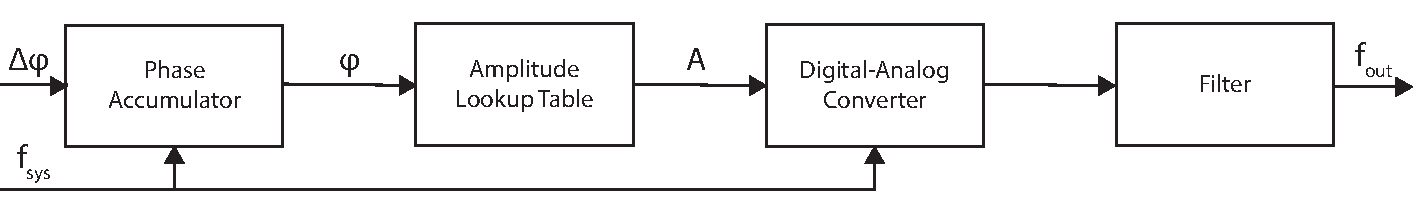
\includegraphics[width=\textwidth]{\figuredir{digital-signal-synthesis/simple-architecture.pdf}}
  \captionsetup{width=.8\textwidth}
  \caption{Signal flow through a simple \gls{dds}. The output frequency
    determines a phase step by which the accumulator is incremented at each
    clock cycle. The value of the phase accumulator is used for amplitude
    lookup of the desired output signal shape. A \gls{dac} outputs the signal
    which then is filtered to smooth the discrete \gls{dac} output.
  }\label{fig:dds_simple_architecture}
\end{figure}
For every clock cycle the phase accumulator is incremented by $\Delta\varphi$.
On overflow of the accumulator a new signal period starts. The phase
accumulator value is used to lookup the corresponding amplitude value of the
desired output signal shape. For example one can use a lookup table with the
values of a sinusoidal output signal. Alternatively one can omit the lookup
table and output a sawtooth output signal by suppling the phase accumulator
output directly to the \gls{dac} or a square wave signal output by suppling
the most significant bit directly. Finally a \gls{dac} converts the digital
amplitude value to an analog signal. An optional analog filter can be used to
smooth the discrete output. In \Cref{fig:dds_simple_output} the signal at the
different processing stages inside a simple \gls{dds} are presented for a
\SI{8}{\bit} precision, system clock frequency
$f_\text{sys}=\SI{1}{\giga\hertz}$ and output frequency
$f_\text{out}=\SI{100}{\mega\hertz}$.
\begin{figure}[ht]
  \centering
  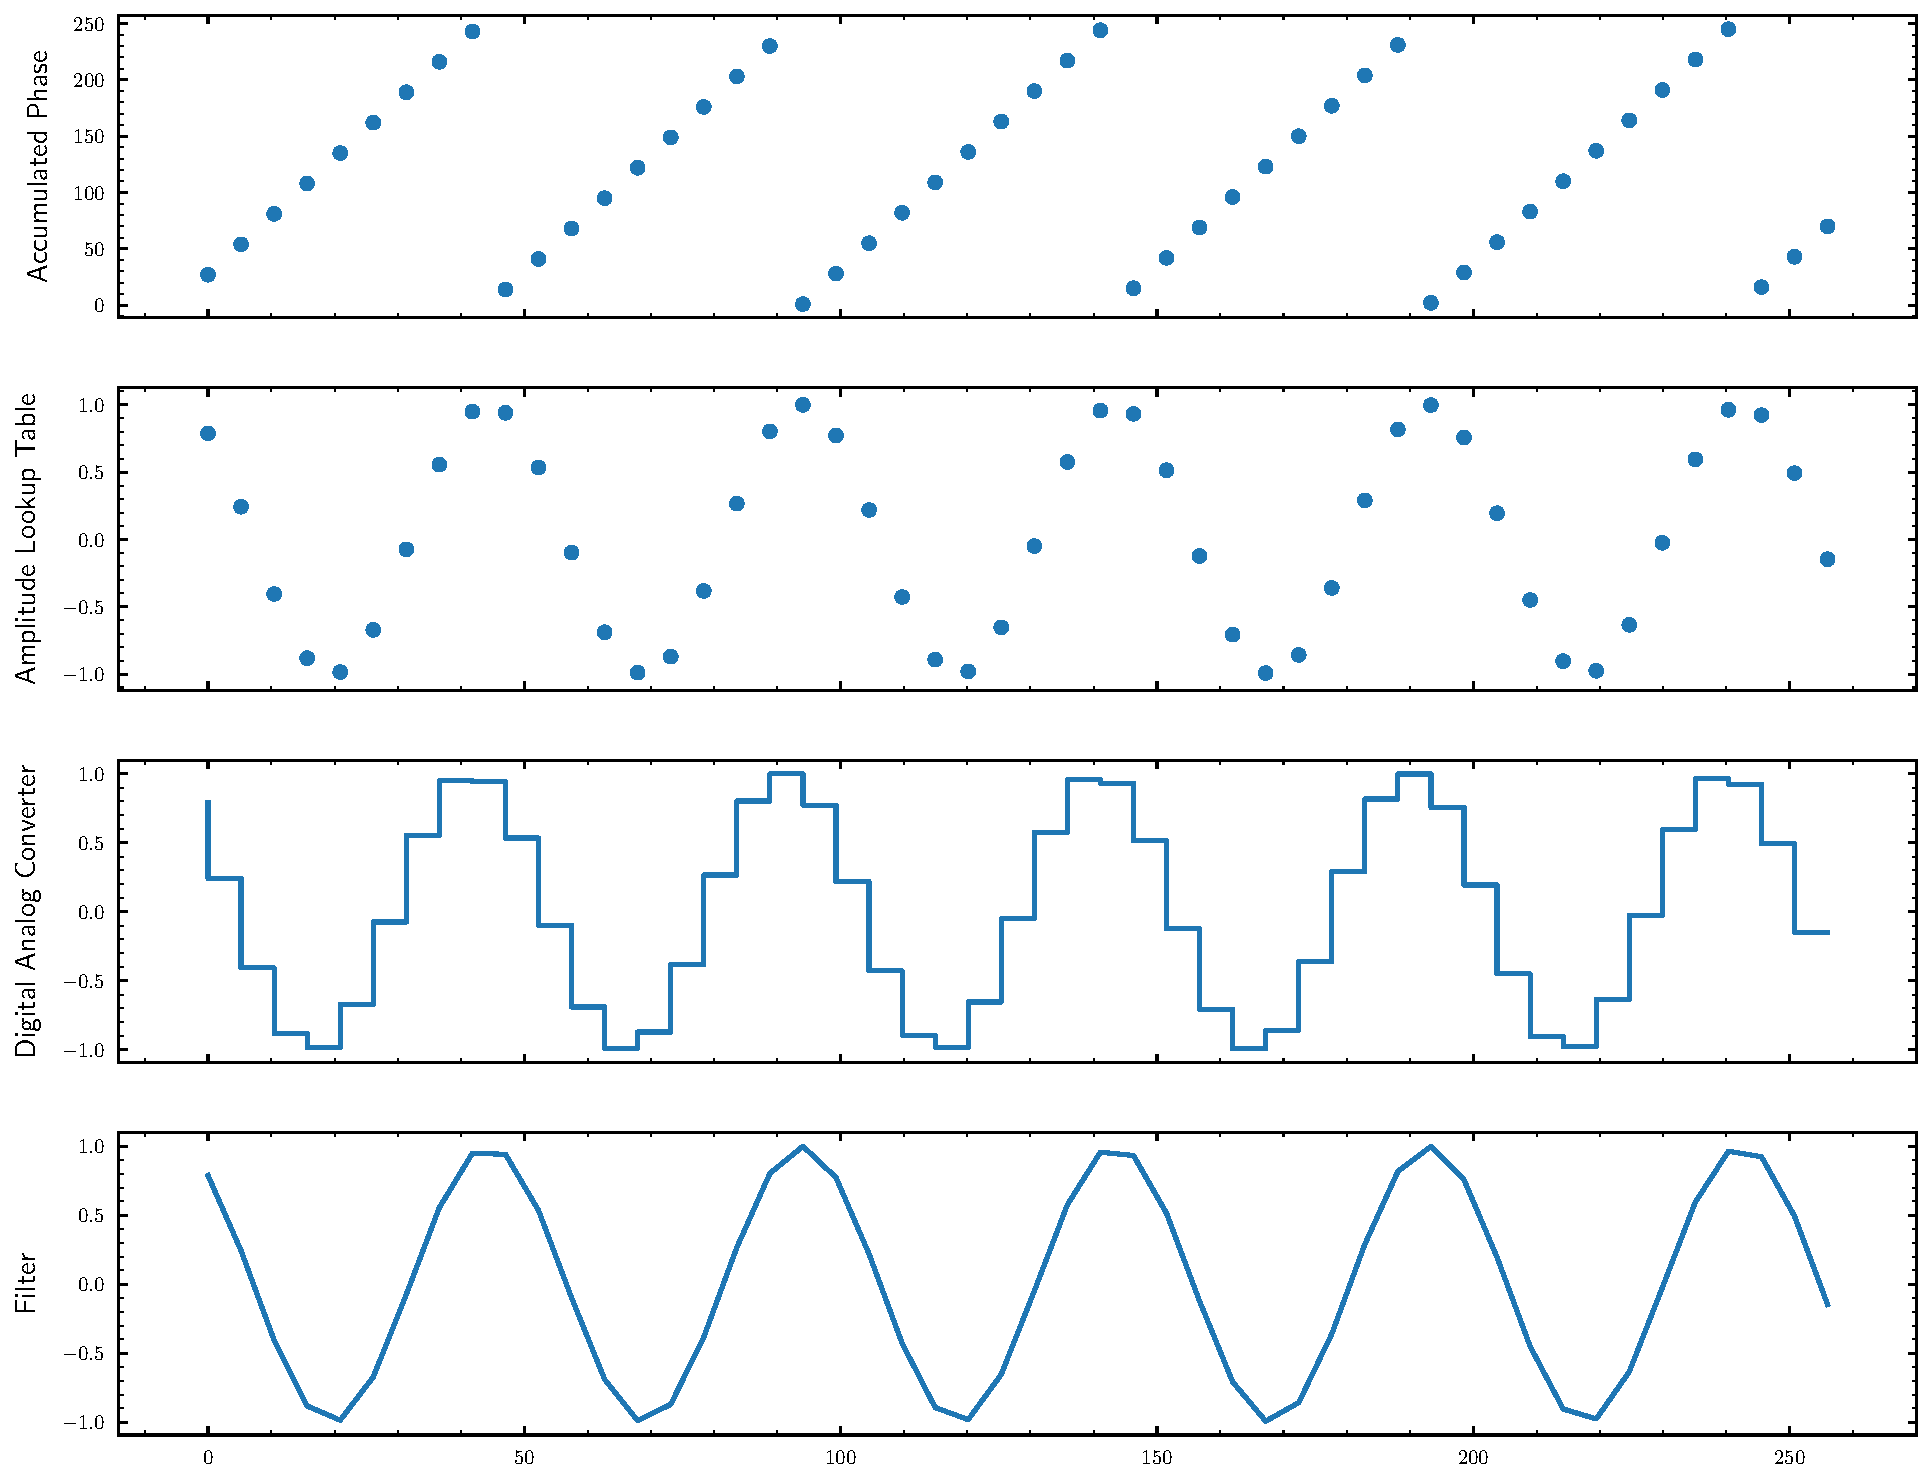
\includegraphics[width=\textwidth]{\figuredir{digital-signal-synthesis/simple-output.pdf}}
  \captionsetup{width=.8\textwidth}
  \caption{Signal outputs at different stages in a simple \gls{dds}. The
    phase accumulator is incremented at each clock cycle by $\Delta\phi$. The
    phase accumulator value is used to lookup a sinusoidal amplitude value
    that is supplied to a \gls{dac}. The final result is smoothed using a
    filter.}\label{fig:dds_simple_output}
\end{figure}
In the first column of \Cref{fig:dds_simple_output} we can see how the phase
accumulator is incremented on every clock iteration and resets on overflow.
In the second column the lookup table has been used to return the
corresponding cosine amplitude. We can see a difference in output shape
between even and odd samples. This is caused by the fact that the phase
increment is not a divisor of the phase accumulator size and we will later
discuss workarounds.

\subsection{Clock generation}

The Nyquist-Shannon sampling theorem states that for a given sample rate a
perfect reconstruction is guaranteed possible for
$f_\text{out}<f_\text{samp}/2$. Until now we have considered the system clock
frequency $f_\text{sys}=f_\text{samp}$ as given. In practice reliable
reference signals are clocked below the desired output range and thereby
cannot directly be used as system clock according to the Nyquist-Shannon
sampling theorem.
\begin{figure}[ht]
  \centering
  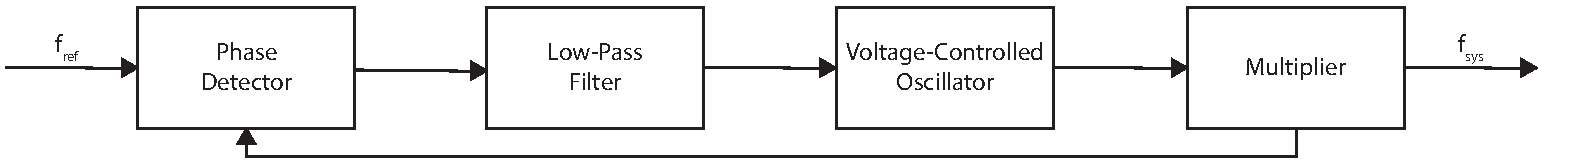
\includegraphics[width=\textwidth]{\figuredir{digital-signal-synthesis/clock-generation.pdf}}
  \captionsetup{width=.8\textwidth}
  \caption{Clock generation signal generation with \gls{pll} and multiplier.
    The phase detector compares the output system phase with the reference
    phase and yields a non-linear error response. The low-pass filter removes
    fast oscillations. The \gls{vco} changes the output phase in dependence
    of the error response. Finally system and reference phase will go in lock.
    }\label{fig:dds_clock_generation}
\end{figure}
\Cref{fig:dds_clock_generation} the system clock generation from a reference
signal is illustrated. The phase detector yields a non-linear error response
comparing the output signal phase with the reference signal phase. After a
low-pass filter removes fast oscillations a \gls{vco} changes its phase
proportional to the error signal. Finally a frequency multiplier creates
harmonics of the reference frequency and extracts a programmed frequency
multiple of $M$ such that the system frequency relates to the reference
clock by $f_\text{sys}=Mf_\text{ref}$ with $1<M\in\mathbb{N}$.

\subsection{Parameter modulation}

So far we only discussed the case of frequency modulation. We will see that
the previous architecture can be easily extended to support amplitude
and phase modulation too.
\begin{figure}[ht]
  \centering
  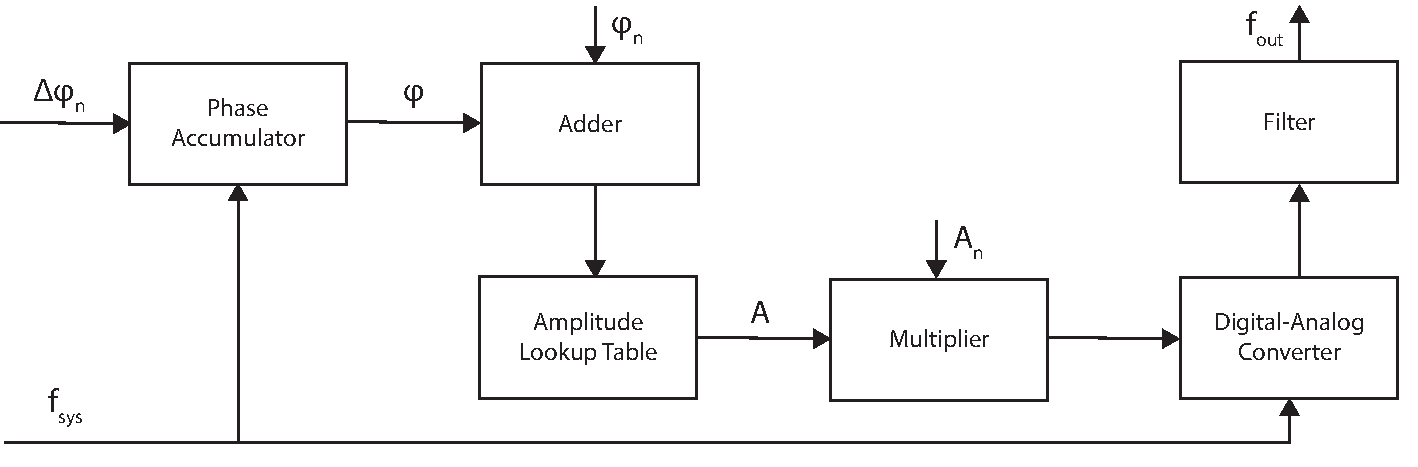
\includegraphics[width=\textwidth]{\figuredir{digital-signal-synthesis/modulation-architecture.pdf}}
  \captionsetup{width=.8\textwidth}
  \caption{
    \gls{dds} architecture supporting modulation of frequency, amplitude and
    phase offset parameters. Phase accumulator increment is now time dependent.
    The phase offset is also time dependent is added as last step to the
    phase accumulator before supplied to the \gls{dac}. The time dependent
    amplitude parameter is multiplied with the amplitude obtained from the
    lookup table.
    }\label{fig:dds_modulation_architecture}
\end{figure}
In \Cref{fig:dds_modulation_architecture} we can see one realization of an
architecture that supports amplitude, frequency and phase modulation. The main
components are the same as in \Cref{fig:dds_simple_architecture}. In addition
we have an adder for a time dependent phase offset and a multiplier for the
digital amplitude value obtained from the lookup table. The time dependence
of the parameters can be either determined by reading from memory or through
generation of another circuit. In a later section we will discuss the case of
a linear frequency sweep provided by a digital ramp.

\section{Quantization errors}
\section{Frequency response}

\section{Operating range}

We apply a reference signal of
\begin{equation}
  f_\text{ref}=\SI{10}{\mega\hertz}
\end{equation}
configured to be used with a \gls{pll} multiplier of
$N=100$ yielding a system clock of
\begin{equation}
  f_\text{sys}=Nf_\text{ref}=\SI{1}{\giga\hertz}.
\end{equation}
The timer clock used for the linear ramp and memory playback runs with
a quarter of the system clock
\begin{equation}
  f_\text{timer}=f_\text{sys}/4=\SI{250}{\mega\hertz}.
\end{equation}

The \gls{ad9910} uses a \SI{14}{\bit} \gls{asf} and \SI{32}{\bit} \gls{ftw}
to parameterize amplitude $A(t)$ and output frequency $f(t)$ by
\begin{align}
  FTW
  :=
  \left\lfloor2^{32}\left(\frac{f_\text{out}}{f_\text{sys}}\right)\right\rceil
  &&
  ASF
  :=
  \left\lfloor\frac{A_\text{out}}{2^{14}}\right\rceil
  \label{eq:elec:ftwasf}
\end{align}
wherein $\lfloor{\cdot}\rceil$ rounds the given float to the nearest integer.
The theoretical limit for the maximum output frequency then is found via
\begin{equation*}
  f_\text{max}
  =
  \left(1-\frac{2^{31}-1}{2^{32}}\right)f_\text{sys}
  =
  \left(\frac{1}{2}-\frac{1}{2^{31}}\right)f_\text{sys}
  \approx
  \frac{1}{2}f_\text{sys}
  =
  \SI{500}{\mega\hertz}.
\end{equation*}
Yet the datasheet \cite{AD9910} reports $f_\text{max}=\SI{420}{\mega\hertz}$
and in fact we found the output signal to be very noisy at the theoretical
limit.

We continue with the assessment of the digital ramp that does a unidrectional
linear sweep on the frequency from \SI{90}{\mega\hertz} to
\SI{110}{\mega\hertz}. The digital ramp of the \gls{ad9910} lets us define
a \gls{ftw} step $M$ word of \SI{32}{\bit} as well as a step rate word $S$ of
\SI{16}{\bit} resolution. They relate to the frequency step and the time
step through
\begin{align}
  \Delta f
  =
  \frac{M}{2^{32}}f_\text{sys}
  &&
  \Delta t
  =
  \frac{S}{f_\text{timer}}
  =
  \frac{S}{4f_\text{sys}}.
  \label{eq:elec:step}
\end{align}
The sweep duration is deterimened by $S,M$ through
\begin{equation}
  T_\text{duration}
  =
  \frac{f_\text{upper}-f_\text{lower}}{\Delta f}\Delta t
  =
  2^{32}\frac{f_\text{upper}-f_\text{lower}}{f_\text{sys}}\frac{S/M}{f_\text{timer}}
\end{equation}
for a target sweep duration of $T_\text{duration}=\SI{10}{ms}$ we find
\begin{equation*}
  \frac{S}{M}
  =
  \frac{T f_\text{timer}}{2^{32}}\frac{f_\text{sys}}{f_\text{upper}-f_\text{lower}}
  =
  \frac{10^9}{2^{35}}
  \approx
  \num{2.9104e-2}
  =
  \frac{1819}{62500}
\end{equation*}
the last step can be obtained by best ratio approximation using continued
fractions as for example described in \cite{Ashley2003}. It should be kept in
mind that the best ratio approximation is likable to introduce an error,
therefore realistic durations may differ from the configured value and it
is possible that better approximations exist that allow smaller $\Delta f,
\Delta t$, thus providing a sweep resolution. In the above case the given
time duration translates to
\begin{align*}
  \Delta f
  =
  \frac{62500}{2^{32}}f_\text{sys}
  \approx
  \SI{145}{\kilo\hertz}
  &&
  \Delta t
  =
  \frac{1819}{f_\text{timer}}
  \approx
  \SI{7.28}{\micro\second}
\end{align*}
or $(f_\text{upper}-f_\text{lower})/\Delta f=138$ discrete data points.

Eventually we are left with the assessment of the amplitude sequence. The
memory fits at most 1024 discrete amplitude values and the \gls{ad9910}
allows us to set the time spent at each amplitude value via the \SI{16}{\bit}
playback rate $P$ word
\begin{equation}
  \Delta t
  =
  \frac{P}{f_\text{timer}}
  =
  \frac{4P}{f_\text{sys}}
\end{equation}
which gives us range from $\min\Delta t=\SI{4}{\nano\second}$ to
$\max\Delta t=\SI{26.14}{\micro\second}$. As we incorporate all of the 1024
data points this gives us a duration range from about
$\min T=\SI{4}{\micro\second}$ to $\max T=\SI{26.84}{\milli\second}$.


\chapter{Experimental setup}

The exerimental setup was largely adopted from \cite{Hertlein2017}, amendments
made include the \gls{rf} signal source of the \gls{aod} and an additional
photodiode to measure the deflected beam intensity.

\section{Optics}

The optical setup can be dissect into a closed first section that reduces
the power of the $\SI{532}{\nano\meter}$ laser source from $\SI{10}{\watt}$
to below $\SI{2}{\milli\watt}$ and an open second section for beam deflection.
Both sections are connected through a \gls{smf}.

\subsection{Power reduction}
\label{sec:powerbox}

Because of safety concerns the power reduction section is confined into a
visually sealed superstructure. \Cref{fig:powerbox} reveals the inside of the
power reduction box.

\begin{figure}[h]
  \centering
  \includegraphics[width=\textwidth]{standalone/powerbox.pdf}
  \caption{Optical configuration of the power reduction section.}
  \label{fig:powerbox}
\end{figure}

The laser beam leaving the laser source is polarized by a $\lambda/2$ retarder
plate such that the succeeding high power beamsplitter BS can divert the
majority of the beams power into a high power beam dump.
Afterwards mirrors M1 and M2 direct the beam towards the center of a $2:1$
telescope composed of two lenses L1, L2 with focal lengths
$f_1=\SI{100}{\milli\meter}$ and $f_2=\SI{50}{\milli\meter}$.
An \gls{aom} diffracts the laser beam into multiple orders. Mirrors M3, M4
project theses orders onto a pinhole which is configured to intromit only the
the first order deflection. The intensity of the first order is subject to
amplitude modulation apllied to the \gls{aom}.
Finally a tunable $\lambda/2$ retarder plate can be used to couple the beam
polarization with the \gls{smf}.

\subsection{Beam deflection and detection}
\label{sec:deflection}

The section for beam deflection and detection as disclosed in
\cref{fig:deflection} receives the down-powered laser beam from previously
described section by a \gls{smf}. Hereinafter the beam passes a tunable
retarder plate and beam splitter BS1. The tunable retarder plate can be used
to adjust the beam intensity without having to access the power box.
A second polarizer with cube BS2 is used to branch off a part of the beam
to a photodiode PD1 that is positioned to be at the focal point of lens L1.
Photodiode PD1 is connected via a control system with the amplitude
modulation of the \gls{aom} depicted in \cref{fig:powerbox} to stabilize
the laser intensity against i.e. thermal drifts.

\begin{figure}[h]
  \centering
  \includegraphics[width=\textwidth]{standalone/deflection.pdf}
  \caption{Optical configuration of the beam deflection section.}
  \label{fig:deflection}
\end{figure}

For horizontal and vertical beam deflection two \gls{aod}s are used. A $1:1$
telescope comprised of two lenses L2, L3
each with focal length $f_2=f_3=\SI{250}{\milli\meter}$ projects the beam
on a pair of objectives that are built of lenses L4 to L7. The purpose of the
objective pair is to focus the laser on to the atom plane.
Consecutively the laser is reflected by a pair of mirrors M3 and M4 to the
part intended for detection. Lens L8 acts as a camera lens and projects the
beam to infinite focus on to the CCD camera sensor. Cube BS3 forks a portion
of the beam away from the CCD camera on to mirror M5 that guides the beam
towards lens L9 in order to focus the beam onto a second photodiode PD2.

\section{Electronics}

Beforehand we described the optical setups used. Now we want to emphasize
on the electronics how they are integrated into the optical setup.

\subsection{Signal source}

The requirements placed by the two \gls{aod} demand flexible but precise
\gls{rf} sources. Fortunately we can resort to a custom made signal
sources based on the \gls{ad9910} \gls{dds} \cite{AD9910} \gls{ic} that can
operate up to \SI{420}{\mega\hertz} and allows modulation of amplitude,
frequency and phase offset by either a constant value or through a single
digital ramp or playback from a memory sequence.

The signal output of the \gls{dds} is of the form
\begin{equation}
  U(t)=A(t)\sin(2\pi f(t)+\phi(t)).
  \label{eq:dds:signal}
\end{equation}
In the following we will ignore the unsynced phase offset, thus setting
$\phi=0$. In case of the single \gls{dds} which drives the \gls{aom} we
have a constant signal, in that sense we can set $A=1$ and
$f_\text{aom}=\SI{80}{\mega\hertz}$ on \cref{eq:dds:signal}.
In the case of the two \gls{dds} which drive the horizontal and vertical
\gls{aod} we configure the frequency to be controlled by the digital ramp in
order to do a linear frequency sweep from
$f_\text{lower}=\SI{90}{\mega\hertz}$ to
$f_\text{upper}=\SI{110}{\mega\hertz}$, yielding
\begin{align}
  f_\text{aod}(t)
  =
  f_\text{lower} + \frac{f_\text{upper}-f_\text{lower}}{T_\text{duration}}t
\end{align}
wherein $T_\text{duration}>0$ denotes the sweep duration. The amplitude is
controlled by memory playback. Given a discrete set of amplitude values
$A_i\in[0,1]$ with $i=1,\dots,N=1024$ the amplitude of the \gls{aod} can be
formulated as
\begin{align}
  A_\text{aod}(t)
  =\sum^N_{i=1}A_i\mathbb{1}_{B_i}(t)
  &&
  B_i:=\left[iT_\text{interval}, (i+1)T_\text{interval}\right[
\end{align}
wherein $T_\text{interval}>0$ denotes the playback interval and
$\mathbb{1}_{B_i}$ is the characteristic function on the set $B_i$.

So far we have assumed $f_\text{aod}(t)$ to be continous and
$T_\text{interval},T_\text{duration}>0$ to be arbitrary, however the internals
of the \gls{ad9910} impose theoretical restrictions on the possible operating
ranges.

\subsection{Signal amplifier}

We use three signal amplifiers with respective input from the signal sources
to have an output power of about $P=\SI{2}{\watt}$ required by the \gls{aod}s
and \gls{aom} for ideal operation. The used amplifiers offer a second input
for external amplitude modulation. In case of the \gls{aom} we connect this
input with the intensity controller.

\subsection{Intensity controller}

The intensity controller is connected to photodiode PD1 that converts the
laser intensity to an input voltage signal of the controller. Given the
input signal we can configure the controller for a reference input voltage.
The controller will then compare the input voltage with set reference voltage
and output an error signal that is proportional to the deviation of the
input from the reference voltage. The inverted error signal is feed to the
signal amplifier connected with the \gls{aom}.

In one attempt we tried to use the intensity controller to compensate for
frequency dependent intensity changes during frequency sweep of the \gls{aod},
however we found that even slow sweep times of $\SI{2}{\second}$ could not
be balanced, therefore the intensity controller only compensates for slow
intensity shifts caused by thermal stress of the laser source.

The intensity controller has to be connected correctly with photodiode PD1
of the setup as well as signal amplifier of the signal that drives the
\gls{aom}.

\begin{figure}[h]
  \centering
  \includegraphics[height=6cm]{example-image-a}
  \caption{The intensity controller next to the \gls{aom} amplifier.}
  \label{fig:intcontrol}
\end{figure}

The XY can be tuned to set the reference signal.

\subsection{Trigger source}

To syncronize the signal sources, the \gls{ccd} camera and the oscilloscope
it was necessary to design a global trigger source that outputs a rising edge
signal to multiple devices and exposes a network programable interface.

\begin{figure}[h]
  \centering
  \includegraphics[height=6cm]{example-image-a}
  \caption{The trigger source exposes a network programable interface and
  provides enough power to drive four output signals.}
  \label{fig:elec:trig}
\end{figure}
The schematics and board layout can be found in the
\cref{app:electronics:trigger_hub}.

\section{Acousto-Optics}

\subsection{Modulator}
\subsection{Deflector}

\section{Assessment}

With the previously described calibration steps in place we can assess the
final quality of the beam with an image capture of the \gls{ccd} camera in the
aligned setup \cref{sec:deflection}.

\begin{figure}[ht]
  \centering
  \includegraphics[width=.5\textwidth]{\figuredir{camera/profile2d.pdf}}
  \caption{Image detail from the captured beam with the \gls{ccd} camera.}
  \label{fig:beamprofile:2d}
\end{figure}

The two dimensional beam profile shows the characteristical two dimensional
gaussian distribution with diffraction rings caused by beam clipping at
finite apertures as described in \cite{Hertlein2017}.

\begin{figure}[ht]
  \centering
  \includegraphics[width=\textwidth]{\figuredir{camera/profile1d.pdf}}
  \caption{1D horizontal and vertical profile extracted from the center of
    the image detail in \cref{fig:beamprofile:2d} with fitted gaussian curve
  and residue.}
  \label{fig:beamprofile:1d}
\end{figure}

By inspecting the one dimensional profiles with fitted gaussian and residue
we again confirm conclusions drawn in \cite{Hertlein2017}. The clipped top
of the measured intensity originates from the saturated pixels of the
\gls{ccd} camera and can be ignored. We further observe a slight assymmetry
at the diffraction rings. Overall the shown profiles can be considered to
confirm a good alignment.

\chapter{Radio electronic characteristics}

By the time the \gls{rf} signal has reached the acoustic transducer, it has
been synthesized from a reference signal, amplified, and matched to the
impedance of the \gls{aod} transducer. We are going to inspect the \gls{rf}
signal characteristics at each transmission and find that each stage
unintentionally carries out frequency dependent amplitude modulation which,
as we will see in the next chapter, is responsible for the complex intensity
distribution observed with the photodiode.

\section{Digital signal synthesizer}

We already covered the fundamental functionality of the \gls{dds} in XX and
its integration in our experimental setup in YY. In this section we want to
check up on the suspected characteristics disclosed in these sections through
real world measurements.

\subsection{Discrete frequency spectrum}

\begin{figure}[h]
  \centering
  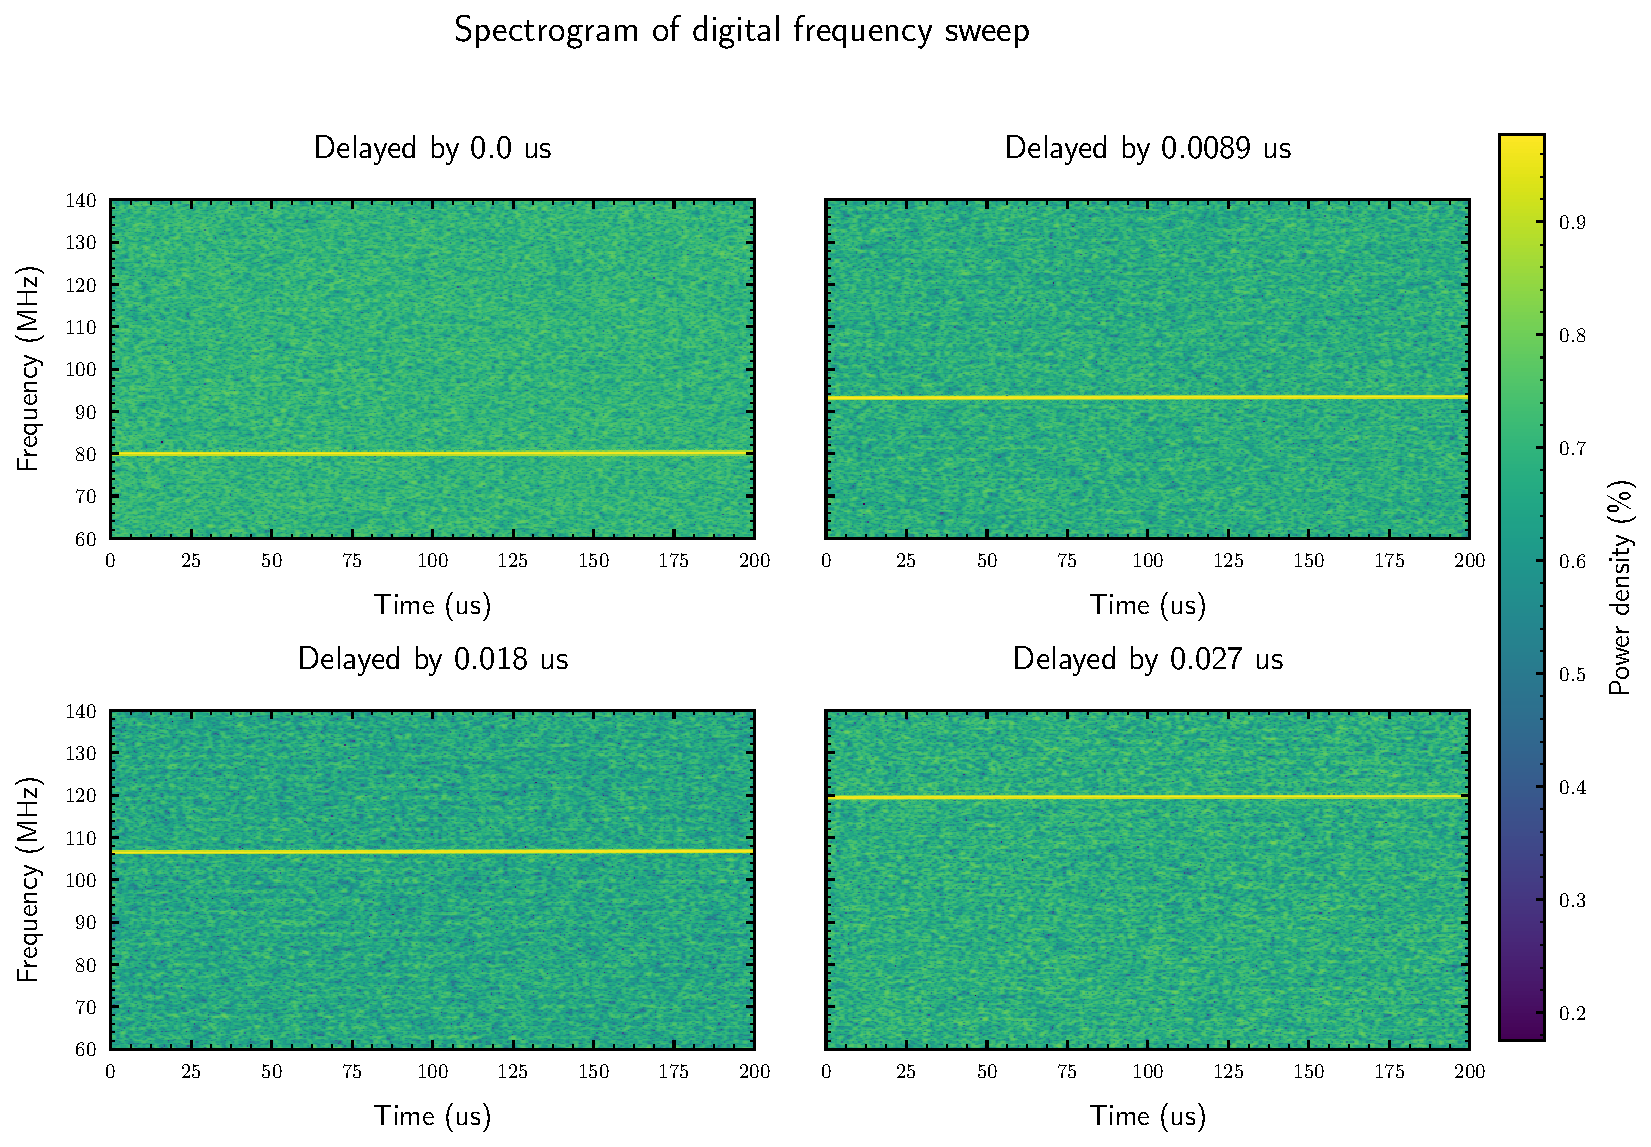
\includegraphics[width=\textwidth]{\figuredir{signal/synthesis/spectrogram.pdf}}
  \captionsetup{width=.8\textwidth}
  \caption{Spectrogram of delayed time windows of the \gls{dds} output signal
    configured to perform a frequency sweep from \SI{80}{\mega\hertz} to
    \SI{120}{\mega\hertz}. For an ideal linear sweep we would expect a linear
    timeline of the frequency, instead we observe a discrete set of
    frequencies which reflects the digital nature of the \gls{dds}.}
  \label{fig:signal_synthesis_spectrogram}
\end{figure}

\subsection{Amplitude frequency response}

\section{Amplifier}

\subsection{Transmission spectrum}

\subsection{Amplitude frequency response}

\section{Acoustic transducer}

\subsection{Reflection spectrum}

\chapter{Acousto-optic intensity transmission}

In the previous chapter we seeked for different aspects of the \gls{rf}
signal powering the \gls{aod} elements. Down the road we had to realize that
there are many forces at work which at large are difficult to account for.
That in mind we proceed with the analysis of the deflected laser beam
intensity subject to the configured frequency and relative amplitude of the
synthesized output \gls{rf} output signal.

\section{Intensity control}

The laser intensity is regulated by a control loop with \gls{aom} in order to
intercept power drifts from the laser source. This control loop is tightly
integrated into our experimental setup and thus will be present for all
subsequent intensity measurements. In this section we want to discuss the
grade of this control loop and estimate its error contribution.

\subsubsection{Experimental setup}

\begin{figure}[h]
  \centering
  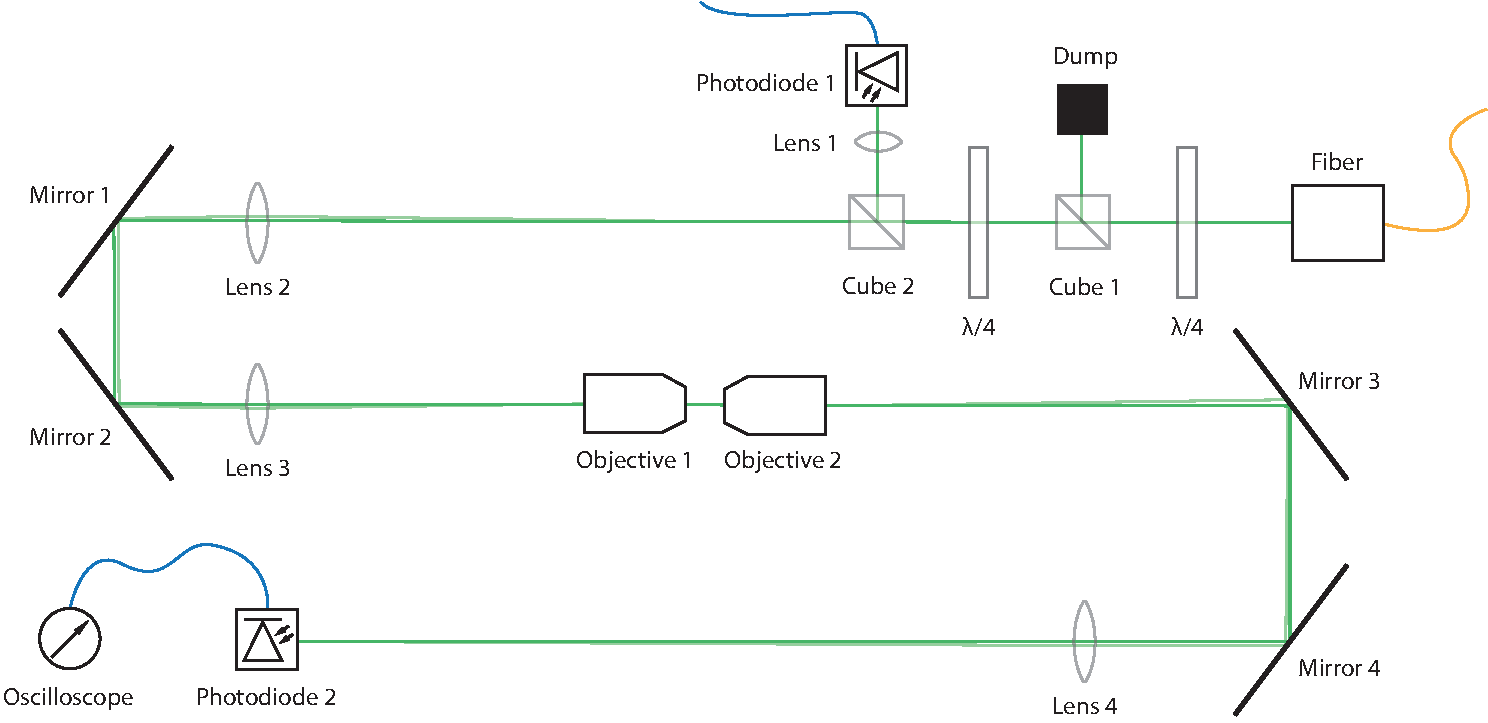
\includegraphics[width=\textwidth]{\mediadir{setup/intensity-control.pdf}}
  \captionsetup{width=.8\textwidth}
  \caption{Optical and electronic setup of the intensity control experiment.
  The \gls{aod}s have been removed. The beam hits photodiode 2 that is
connected to the oscilloscope.}
  \label{fig:intensity_control_setup}
\end{figure}

The experimental setup is the same as described in XX but with disassembled
\gls{aod} and photodiode 2 as the terminus of the laser beam. The setup is
depicted in \Cref{fig:intensity_control_setup}. The photodiode gain was set
to \SI{50}{\decibel}.

\subsection{Long term measurement}

In the long term measurement we were interested in the long term behaviour
of the intensity control loop. In particular if there are oscillations or
intensity collapses.

Therefore we obtained voltage measurements in an interval of about
\SI{2}{\minute} over a total time of approximately \SI{16}{\hour}.

\begin{figure}[ht]
  \centering
  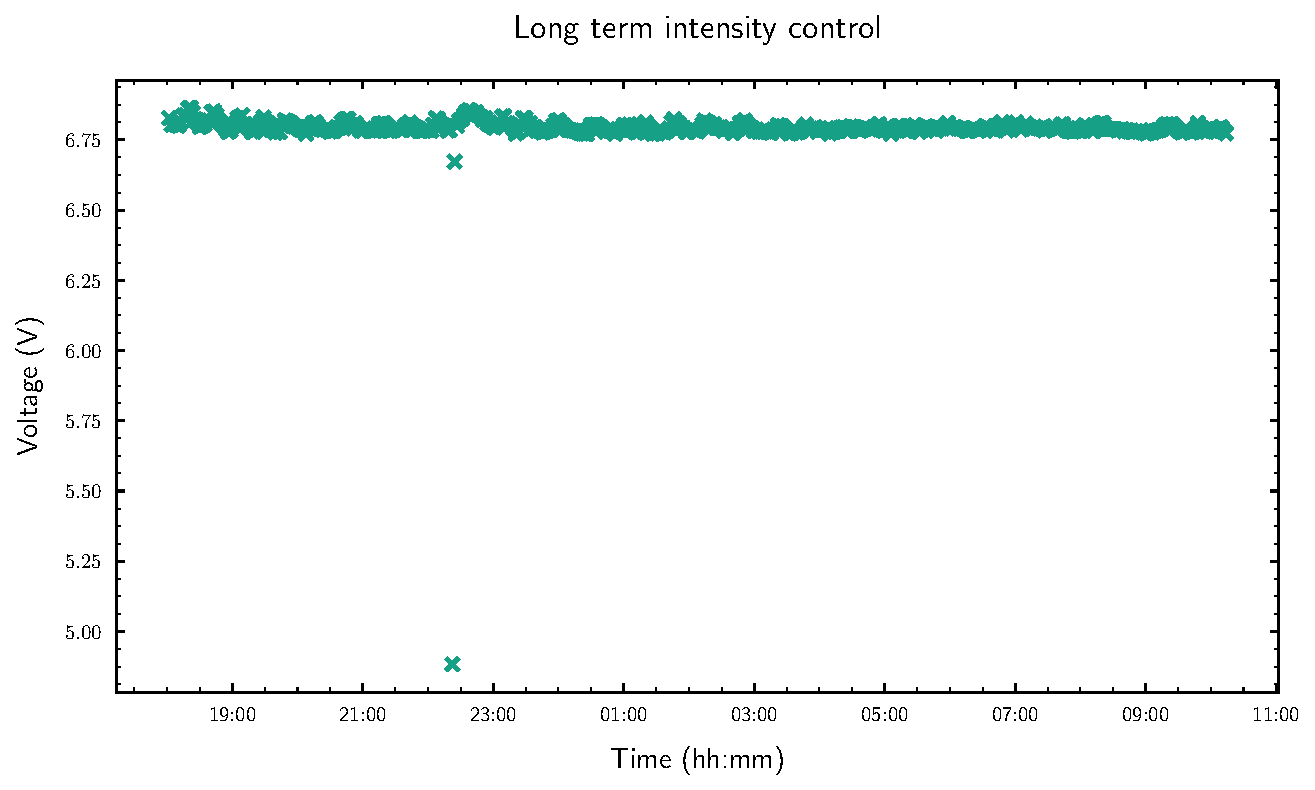
\includegraphics[width=\textwidth]{\figuredir{intensity/control/long.pdf}}
  \captionsetup{width=.8\textwidth}
  \caption{Long term measurement of the intensity with controlled intensity.
    The intensity was measured every \SI{2}{\minute} for over \SI{16}{\hour}
    to determine the accuracy of the intensity controller. The outlier at
    about 22:45 was caused by laboratory visit otherwise the intensity remains
  stable.}
  \label{fig:intensity_control_long}
\end{figure}

The voltage time series is shown in \Cref{fig:intensity_control_long}. We 
note outliers at about 22:45 which were probably caused by a late laboratory
visit. Further we see a constant albeit noisy intensity signal. In comparison
we could watch real time oscillations and drifts when disabling the control
loop.

\Cref{tab:intensity_control_long} depicts the descriptive statistics belonging
to the voltage time series visualized in \Cref{fig:intensity_control_long}.
The mean intensity is measured to be around \SI{6.79}{\volt} with peaks up
to \SI{6.86}{\volt}. The standard deviation yields us a relative error of
around \SI{1.4}{\percent}.

\begin{table}[h]
  \centering
  \begin{tabular}{|c|c|c|c|}
    \hline
    Mean & Minimum & Maximum & Standard deviation \\
    \hline
    \SI{6.79}{\volt} &
    \SI{4.88}{\volt} &
    \SI{6.86}{\volt} &
    \SI{0.09}{\volt} \\
    \hline
  \end{tabular}
  \captionsetup{width=.8\textwidth}
  \caption{Descriptive statistics of the short term measurement of the
  intensity with controlled intensity. Note the small standard deviation.}
  \label{tab:intensity_control_long}
\end{table}

\subsection{Short term measurement}

The previous section gave us already some good insights about the long term
stability of the intensity control loop. Yet in practice typical intensity
measurements are of much smaller magnitude, henceforth it seems close at hand
to also conduct a short term measurement.

\begin{table}[h]
  \centering
  \begin{tabular}{|c|c|c|c|}
    \hline
    Mean & Minimum & Maximum & Standard deviation \\
    \hline
    \SI{6.78}{\volt} &
    \SI{6.77}{\volt} &
    \SI{6.82}{\volt} &
    \SI{0.01}{\volt} \\
    \hline
  \end{tabular}
  \captionsetup{width=.7\textwidth}
  \caption{Descriptive statistics of the short term measurement of the
  intensity with controlled intensity. Note the small standard deviation.}
  \label{tab:intensity_control_short}
\end{table}

For the short term measurement time parameters were adjusted to a sample
interval of \SI{10}{\second} and measurment were performed over \SI{1}{\hour}.

\begin{figure}[ht]
  \centering
  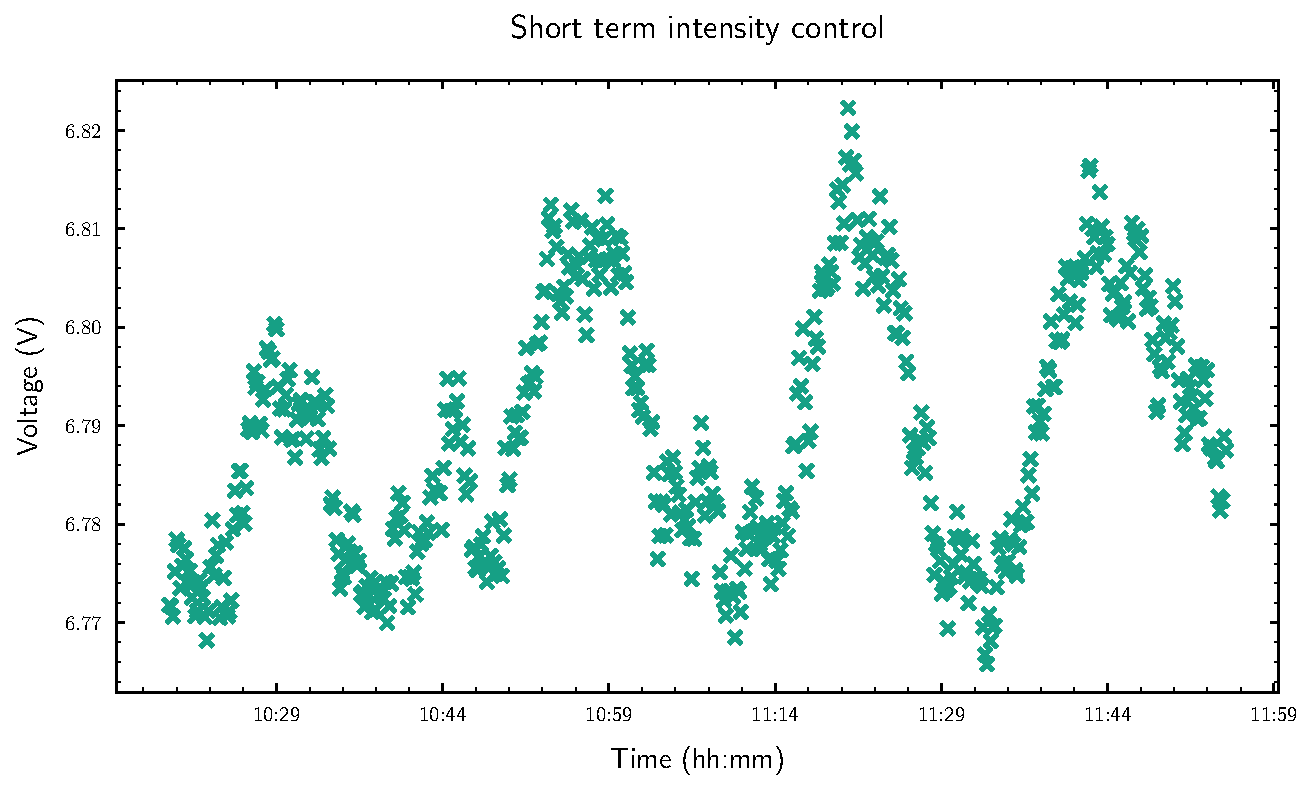
\includegraphics[width=\textwidth]{\figuredir{intensity/control/short.pdf}}
  \captionsetup{width=.8\textwidth}
  \caption{Short term measurement of the intensity with controlled intensity.
    The intensity was measured every \SI{10}{\second} for over \SI{1}{\hour}
    to determine the accuracy of the intensity controller.}
  \label{fig:intensity_control_short}
\end{figure}

The intensity time series of the short term measurement is depicted in
\Cref{fig:intensity_control_short} and the associated descriptive
statistics are presented in \Cref{tab:intensity_control_short}.

On a smaller timescale we see that the intensity control loop performs
periodic oscillations, however the descriptive statistics show much smaller
deviation from the mean, than observed in the long term measurements. As we
do not see outliers in \Cref{fig:intensity_control_short} we can pay more
attention to the value range of \SI{0.05}{\volt} which was obfuscated in
the long term measurement because of outliers.

\subsubsection{Summary}

The previous discussion confirmed that the intensity is regulated in that
we only observe oscillations around the targeted intensity value. Yet we are
still missing statements with regard to the magnitude of these oscillations
as we are missing a comparison to real intensity data.

\begin{table}[ht]
  \centering
  \begin{tabular}{|c|c|c|}
    \hline
    Measurement & Value range & Standard deviation \\
    \hline
    long term & \SI{1.98}{\volt} & \SI{0.09}{\volt} \\
    \hline
    short term & \SI{0.06}{\volt} & \SI{0.01}{\volt} \\
    \hline
    typical & \SI{1.43}{\volt} & \SI{0.40}{\volt} \\
    \hline
  \end{tabular}
  \captionsetup{width=.8\textwidth}
  \caption{Descriptive statistics of the short and long term measurement
  of the intensity control and a typical intensity measurements where we
subtracted the mean intensity for comparison.}
  \label{tab:intensity_control}
\end{table}

For a typical measurement, to compare the intensity oscillations with, we
elected the intensity progression of a linear frequency sweep of the
\gls{aod} in the vertical socket while the \gls{aod} in the horizontal socket
is fixed. We will discuss this specific meausurement in detail in a later
section. In \Cref{tab:intensity_control} we see some statistics of the
long and short term measurements next to the typical measurement.

\begin{figure}[ht]
  \centering
  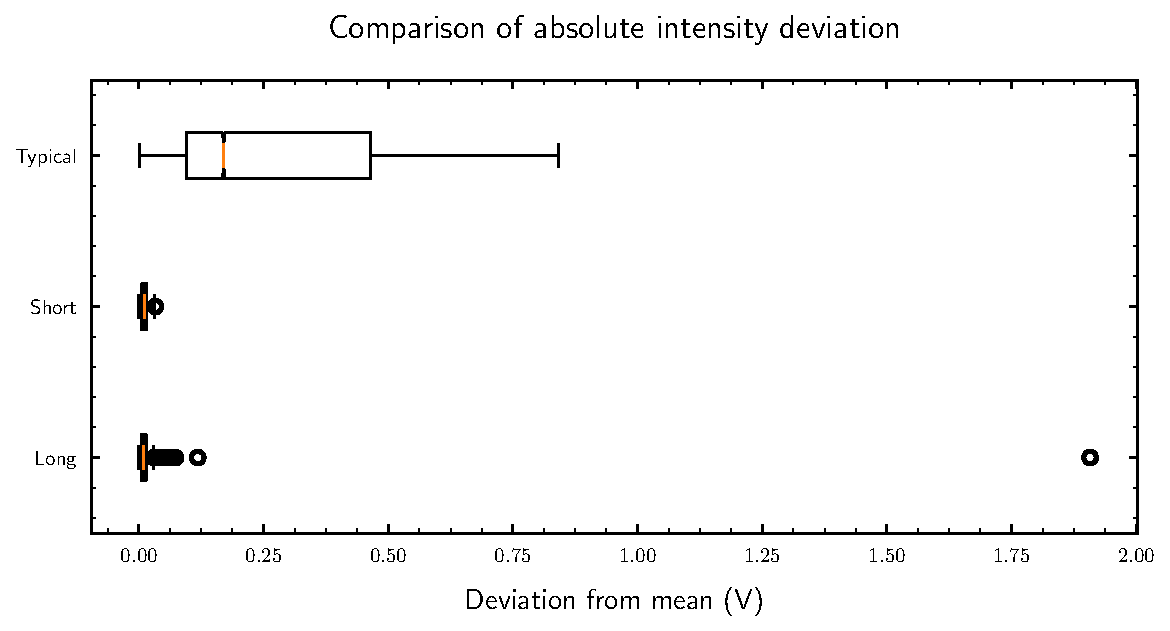
\includegraphics[width=\textwidth]{\figuredir{intensity/control/deviation.pdf}}
  \captionsetup{width=.8\textwidth}
  \caption{Boxplot of the long and short term intensity measurements and a typical
  intensity measurement with the \gls{aod} where we subtracted the mean intensity
  for comparison. The typical measurements covers a much wider intensity range
then deviations from the intensity control loop.}
  \label{fig:intensity_control_comparison}
\end{figure}

One dismally error estimate would be the quotient of the value range of the
short term measurement and the typical measurement, yielding an error of
\SI{4.2}{\percent}. A second approach would be the quotient of the standard
deviation of the short term and typical measurement, yielding
\SI{2.5}{\percent} error. When comparing the typical measurement to the
statictis of a long term measurement we find rather large errors which
suggests that there re other statistical key figures which may be more
suitable.

A boxplot is very useful in visualizing the spread. We have an orange stripe
marking the median, the contour of the box marking the data between first and
third quantil. The usual value range is marked by the whiskers and outliers
are marked as the circles outside the whiskers.
In \Cref{fig:intensity_control_comparison} we see such a boxplot for the
absolute deviation from the mean of the three measurements. The absolute
deviation from the mean accounts for the different transmission just because
of the presence of the \gls{aod} in the typical measurement but keeps the
linear scale unlike the squared deviation from mean. We can see that in a
typical measurement (upper boxplot) the usual deviation from mean is much
larger than for the short and long term measurement of the intensity
regulation.

\section{Spatial beam profile}

We figured out that the intensity control loop operates as expected. Next we
want to assess the quality of our optical alignment to sort out later
systematic measurement errors from poor calibration. One way to assess the
alignment grade of our alignment is to evaluate the spatial profile of the
laser beam with respect to deviations from an ideal gaussian profile.

\subsubsection{Experimental setup}

In the previous setup we used a second photodiode to measure the temporal
deviations of the intensity. In order to measure spatial deviations of the
intensity we replaced the photodiode with a \gls{ccd} camera.

\begin{figure}[ht]
  \centering
  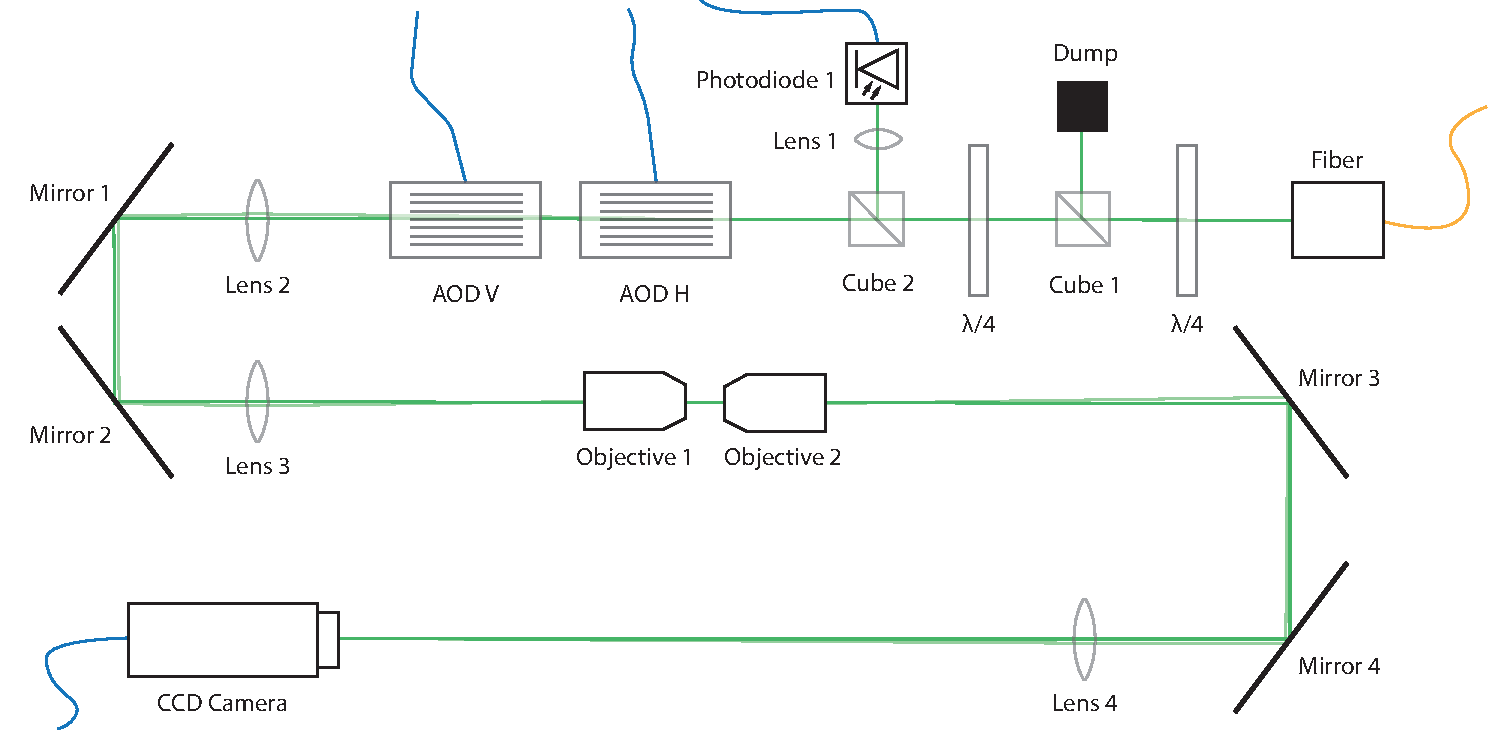
\includegraphics[width=\textwidth]{\mediadir{setup/intensity-profile.pdf}}
  \captionsetup{width=.8\textwidth}
  \caption{The beam is focused onto the \gls{ccd} sensor of the camera. The
    \gls{aod} are configured at \SI{100}{\mega\hertz} center frequency.
  }
  \label{fig:intensity_profile_setup}
\end{figure}

In \Cref{fig:intensity_profile_setup} we see the setup used to measure the
beam profile. The \gls{aod} are configured at \SI{100}{\mega\hertz} center
frequency. The distance between Lens 4 and the \gls{ccd} sensor is chosen
such that the the beam head is focused.

In \Cref{fig:intensity_profile_2d} we can see an enlarged image patch of the
complete image caputre taken with the \gls{ccd} camera. We can see a strong
illuminated circular spot in the center of the iamge with an area of about
\SI{2.5}{\milli\meter}. The intensity inside the spot seems homogeneous,
however this is caused because the pixels are saturated in this area.
We could reduce the intensity or apply an optical filter to the camera to
resolve the intensity gradient inside the spot, but only at the cost of
the intensity distribution around the spot. Around the circular spot we can
see a diffraction ring. The diffraction ring is well described in
\cite{Hertlein2017} and originates from the finite aperture of the objectives.

\begin{figure}[ht]
  \centering
  \includegraphics[width=.5\textwidth]{\figuredir{intensity/profile/profile2d.pdf}}
  \caption{Image detail from the captured beam with the \gls{ccd} camera.}
  \label{fig:intensity_profile_2d}
\end{figure}

Altough \Cref{fig:intensity_profile_2d} gives us a good overview of the
spatial beam profile it is difficult to see deviations from an ideal
gaussian curve in this representation. Henceforth we performed two
perpendicular cuts and visualized the one dimensional spatial beam
distribution in \Cref{fig:intensity_profile_1d}.

\begin{figure}[ht]
  \centering
  \includegraphics[width=\textwidth]{\figuredir{intensity/profile/profile1d.pdf}}
  \captionsetup{width=.8\textwidth}
  \caption{One dimensional perpendicular cut of the two dimensional beam
    distribution from the two dimensional beam profile in
    \cref{fig:intensity_profile_2d} with fitted gaussian curve.}
  \label{fig:intensity_profile_1d}
\end{figure}

In \Cref{fig:intensity_profile_1d} we can clearly observe the effects of
saturation around the center and how we would expect the intensity to be
if we could experimentally resolve it in the Gaussian fit. In contrast to the
ideal Gaussian profile we again observe contributions to the Airy disc around
the otherwise Gaussian profile causes by the finite aperture. Further we can
now clearly observe assymmetry from the intensity contributions around the
Gaussian which means that our alignment is not perfect.

\subsubsection{Summary}

We can confirm the results reported in \cite{Hertlein2017} that the spatial
beam profile equals a two dimensional Gaussian combined with a diffraction
ring caused from the finite aperture of the objectives. Further we observe
slight assymmetries in the diffraction ring suggesting inperfect alignment.

Though assymetries in the spatial beam profile are present, we do not see any
further complications as the intensity measurements with the photodiode will
cover the complete beam profile.

\section{Difference between individual acousto-optic deflectors}

Our optical setup uses a single two dimensional \gls{aod} that comprises two
\gls{aod} elements perpendicular to eachother. At first we want to examine the
behaviour of the single \gls{aod} elements to eachother. In particular we
are interested if and how the \gls{aod} elements differ.

\subsubsection{Experimental setup}

The used 2D \gls{aod} is depicted in \Cref{fig:aod_socket}. We see the
two \gls{aod} elements in the respective horizontal and vertical slot. The
internals of the vertical \gls{aod} (left-hand side) are illustrated. The
element itself spans through the casing (dashed line) while the acousto-optic
crystal (dotted line) is glued onto the element. The laser beam passes through
the acousto-optic crystal. In the following we will refer to the horizontal
\gls{aod} element as the \gls{aod} element anticipated for the horizontal
slot and accordingly to the vertical \gls{aod} element as the \gls{aod}
element intended for the vertical \gls{aod} socket.

\begin{figure}[ht]
  \centering
  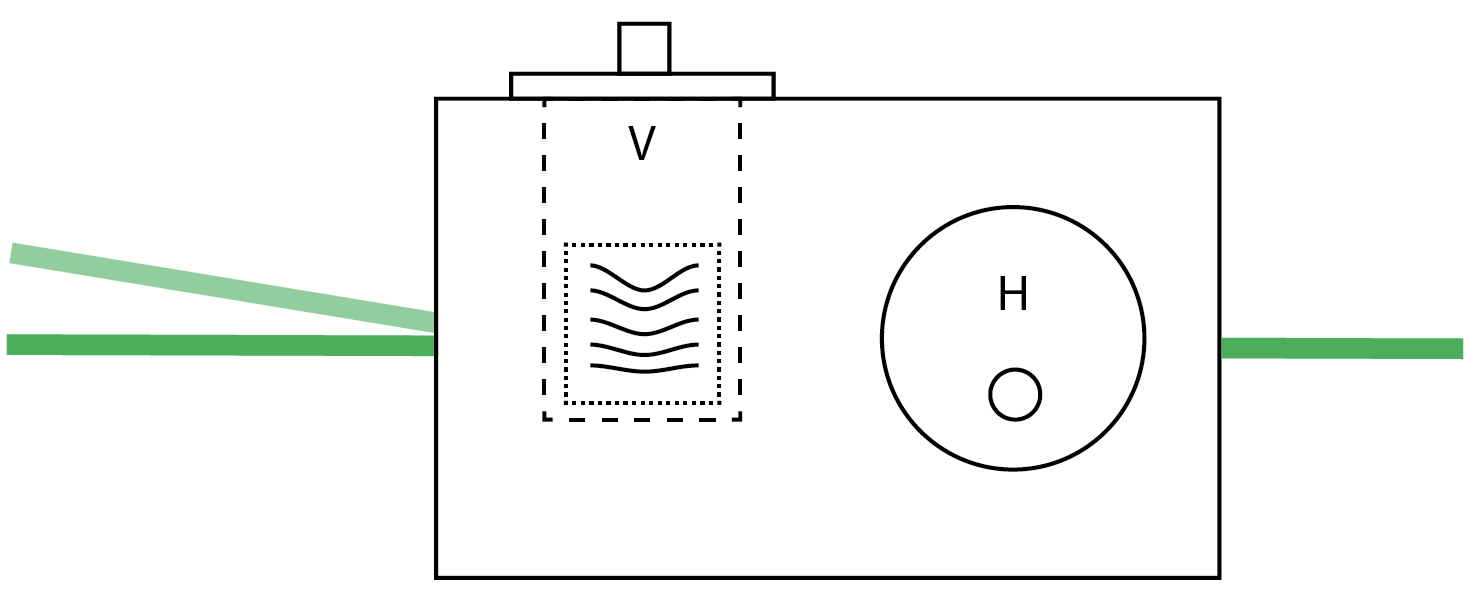
\includegraphics[width=\textwidth]{\mediadir{setup/aod-socket.png}}
  \captionsetup{width=.8\textwidth}
  \caption{The 2D \gls{aod} comprises two perpendicular orientated \gls{aod}
  elements.}
  \label{fig:aod_socket}
\end{figure}

\subsection{Individual acousto-optic deflectors}

For the following experiment we will only leave one \gls{aod} element mounted
in the casing depicted in \Cref{fig:aod_socket}. The other slot will be empty.
Then we will exchange socket positions for each respective \gls{aod} element
and measure the beam intensity subject to the linear frequency sweep from
\SI{80}{\mega\hertz} to \SI{120}{\mega\hertz} over a duration of
\SI{260}{\milli\second} and the configured \gls{dds} amplitude. As \gls{rf}
signal source the amplifier and \gls{dds} combination intended for the
horizontal \gls{aod} element was used to avoid influences of the amplification
offset between the two amplifiers.

The result for the four configurations (horizontal element in horizontal slot,
horizontal element in vertical slot, vertical element in horizontal slot
and vertical element in vertical slot) are visualized as heatmaps in
\Cref{fig:intensity_distribution_unpaired}. The color values are normalized in between the
different heatmaps and can be related to the measured voltage from the
photodiode by the colorbar on the right-hand side.

\begin{figure}[ht]
  \centering
  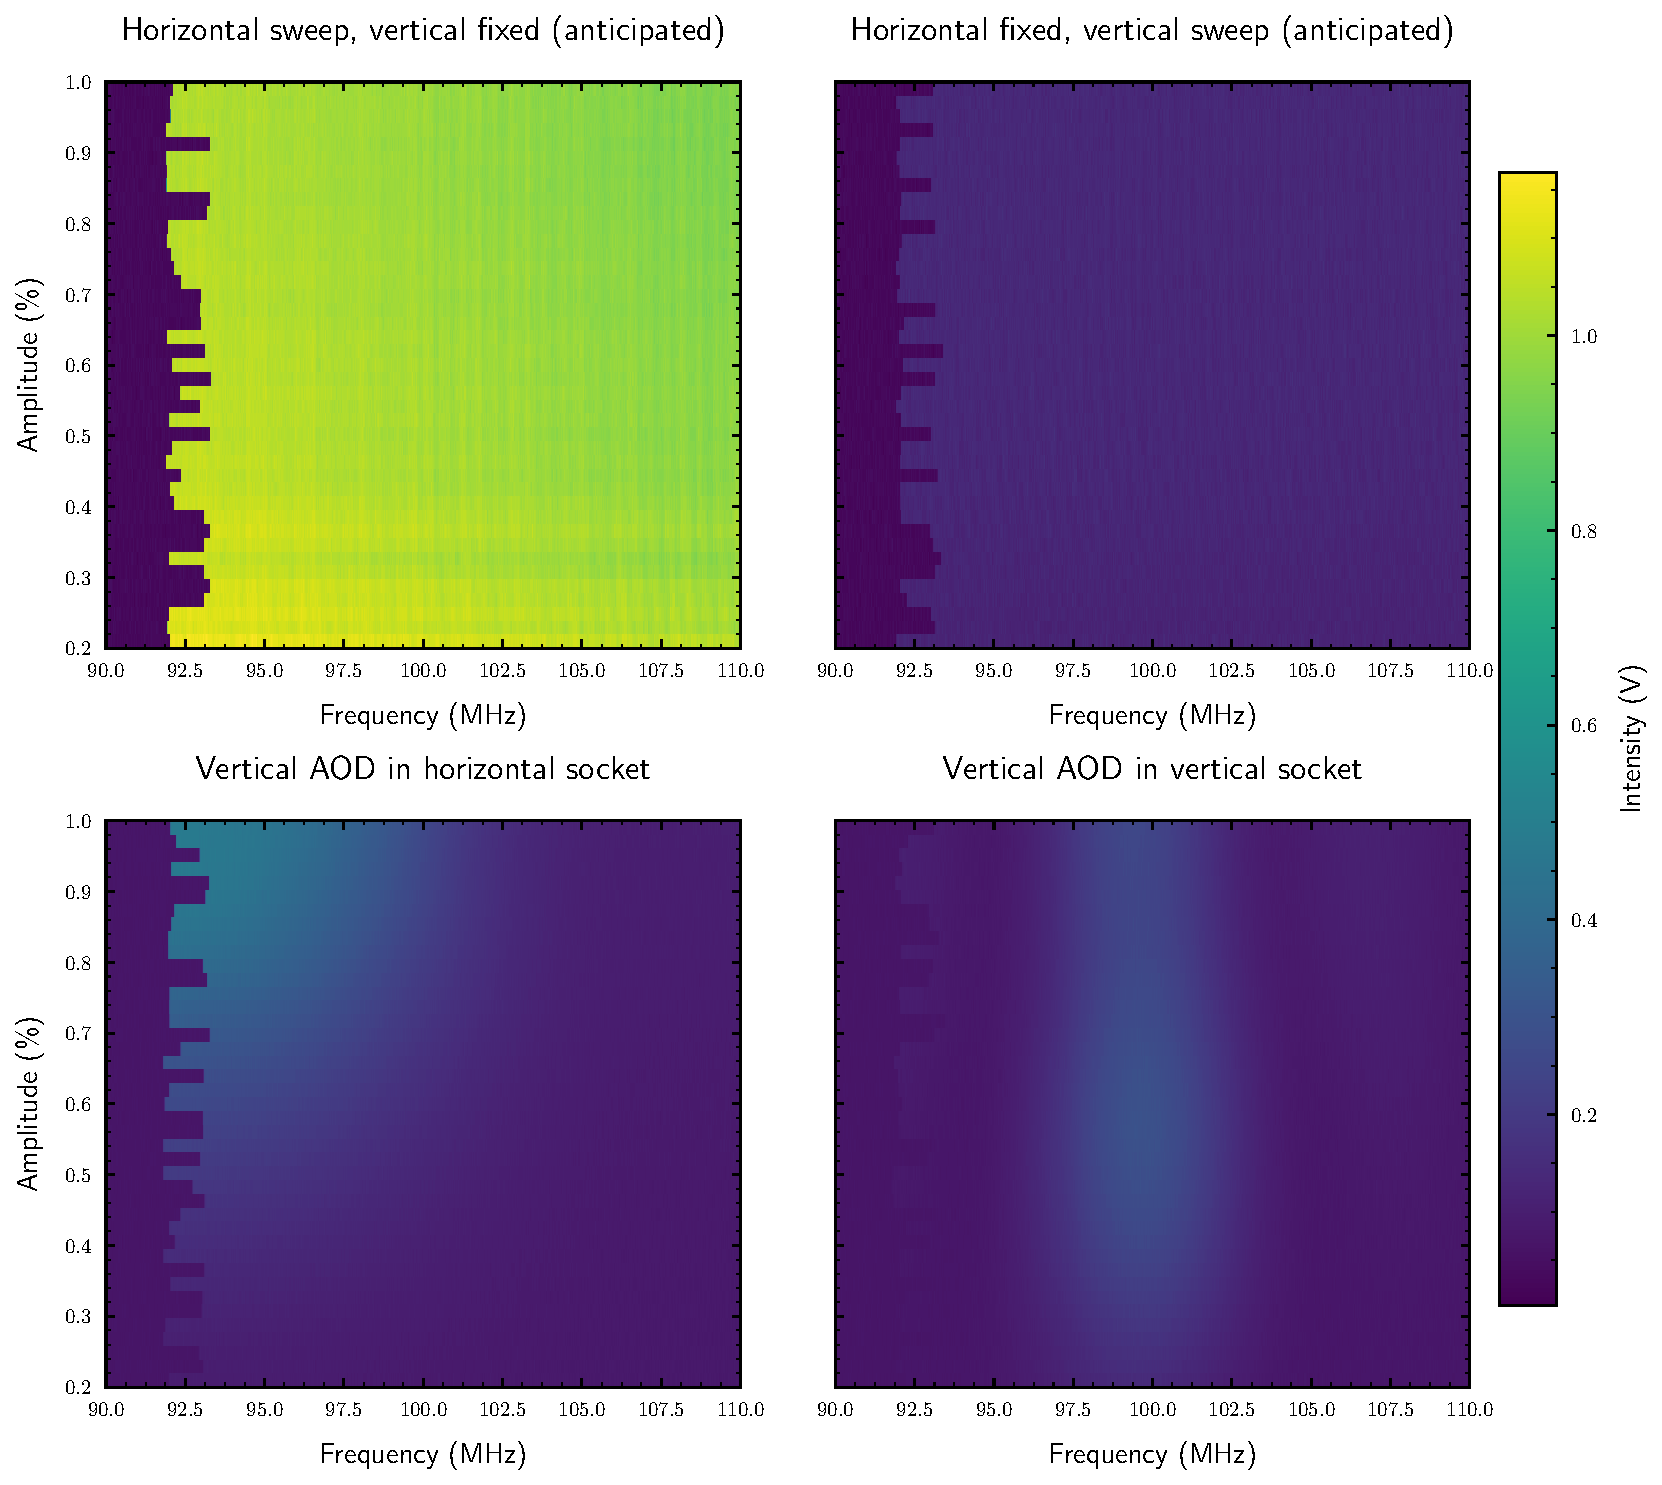
\includegraphics[width=\textwidth]{\figuredir{intensity/distribution/unpaired-amplitude.pdf}}
  \captionsetup{width=.8\textwidth}
  \caption{Intensity distribution over linear frequency sweep at different
  configured \gls{dds} amplitudes for different individual \gls{aod}
configurations.}
  \label{fig:intensity_distribution_unpaired}
\end{figure}

Oddly enough we observe that both \gls{aod} differ strong in their respective
intensity transmission behaviour in dependence of their slot position.
Furthermore we observe that the intensity transmission is much higher in the
case of the horizontal \gls{aod} element mounted to the intended horizontal
slot compared to all other configurations. In addition we can see that for
the horizontal \gls{aod} has an asymmetric, probably non-analytic, intensity
transmission. The highest intensity transmission is obtained for relative
amplitudes configured between \SI{60}{\percent} and \SI{90}{\percent} with
high dependence on the frequency. Another interesting observation is that
the intensity transmission seems very similar for the horizontal element in
the vertical slot and the vertical element in the vertical slot which
map also seems more symmetric with respect to the frequency axis. In fact
for these configurations the configured relative amplitude seems not to
interfere much with the measured voltage at the photodiode.

\subsection{Paired acousto-optic deflectors}

The \gls{aod} elements differ significantly in their intensity transmission
in between and with respect to their position. We find the horizontal element
in the anticipated horizontal position to have a significantly higher
transmission then any other configuration. Therefore we presume that the
\gls{aod} elements have a very high polarization dependency and are concerted
to eachother. We may find more evidence for this hypothesis by mounting both
\gls{aod} elements in their intended and exchanged slots.

\begin{figure}[ht]
  \centering
  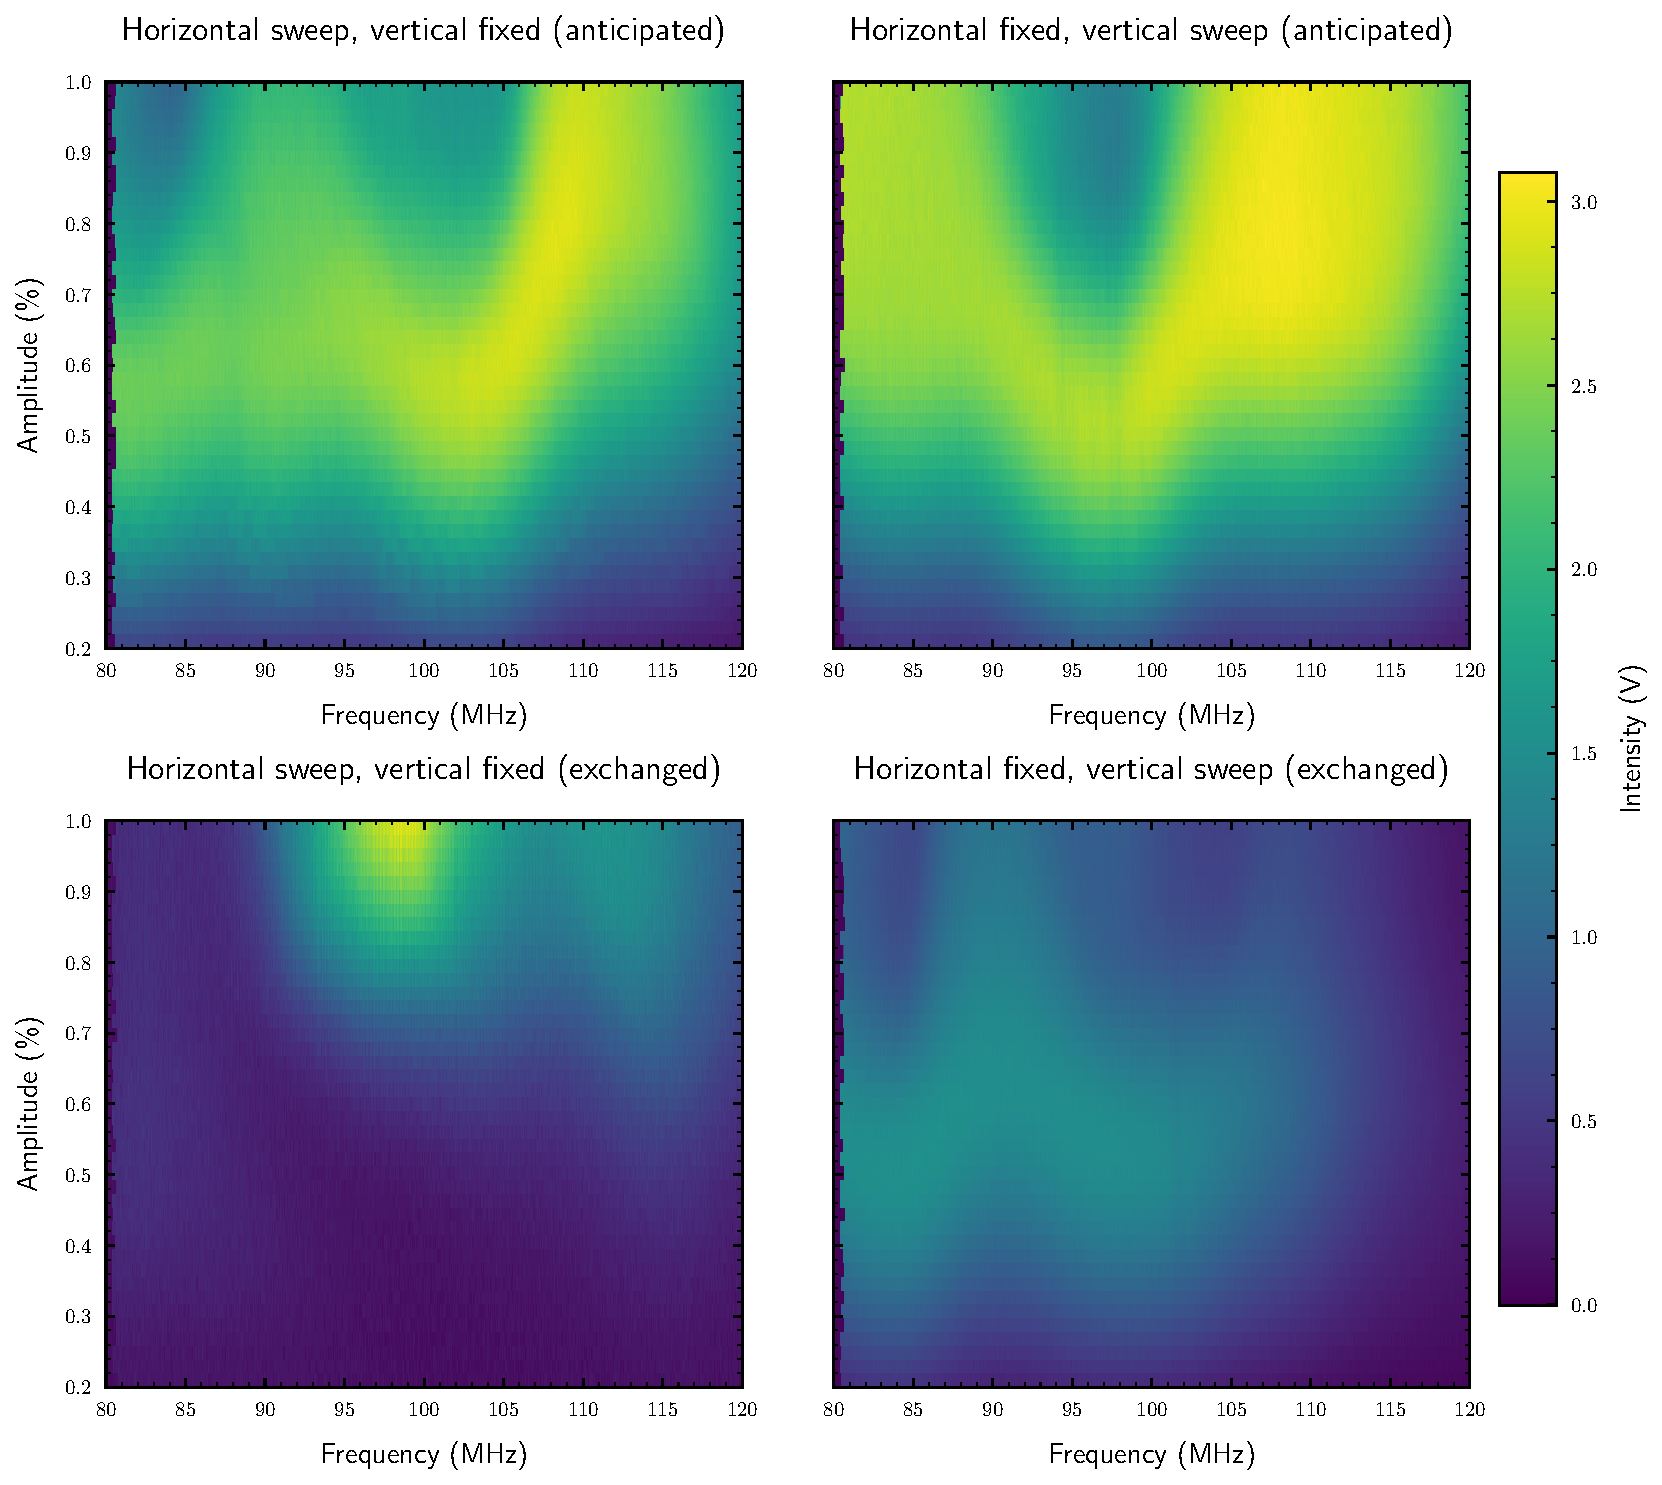
\includegraphics[width=\textwidth]{\figuredir{intensity/distribution/paired-amplitude.pdf}}
  \captionsetup{width=.8\textwidth}
  \caption{Intensity distribution over linear frequency sweep at different
  configured \gls{dds} amplitudes for different individual \gls{aod}
configurations.}
  \label{fig:intensity_distribution_paired}
\end{figure}

In \Cref{fig:intensity_distribution_paired} the measured voltage of the
second photodiode are visualized in a two-dimensional heatmap. The horizontal
axis represents the frequency of the \gls{rf} signal applied to the \gls{aod}
elements whereas the vertical axis the configured \gls{dds} relative
amplitude. In the first row the elements where in their intended slots whereas
we exchanged them for the second row. In the first column the frequency
sweep was applied such that the beam moves along the horizontal axis while
in the second column the frequency sweep was applied to the element that
causes beam movement in the vertical direction.

We see that for the exchanged positions the transmission is reduced and
asymmetric with respect to the sweep direction whereas the elements in their
intended position perform better in every aspect. We therefore conclude that
the \gls{aod} are cut in a intended way to account among others for
polarization effects and it is advised to operate them in their anticipated
slot as we will do for all following experiments.

\subsubsection{Summary}

The transmission of \gls{aod} crystals depends among others on the
polarization mode of the incident laser beam. A two dimensional \gls{aod}
has to be designed around this property and therefore requires the crystals
to be matched to each other.

\section{2D intensity distribution}

In the previous section we sorted out the influence of the \gls{aod} element
position and acknowledged that \gls{aod}s differ significant in their
optical properties. In the present section we now want to explore the
intensity transmission for a two dimensional sweep as intended to be used
for the optical potentials.

\subsubsection{Experimental setup}

The experimental setup is similar to the previous setups and is shown in
\Cref{fig:intensity_distribution_setup}. We have both \gls{aod} mounted in
their anticipated position. The \gls{aod} elements are aligned to maximize
intensity at the center frequency. The laser beam is directed into a second
photodiode where we measure the intensity with respect to the configured
\gls{dds} signal.

\begin{figure}[h]
  \centering
  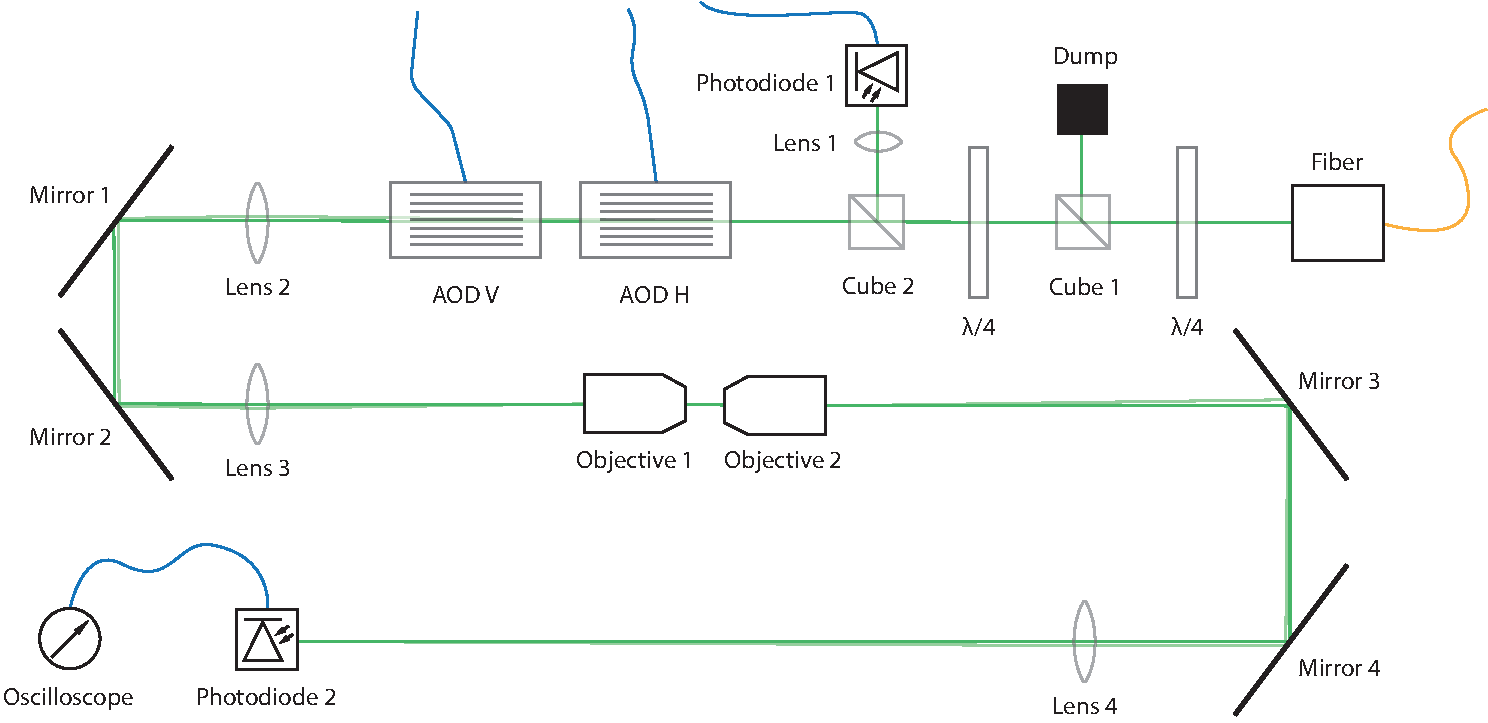
\includegraphics[width=\textwidth]{\mediadir{setup/intensity-distribution.pdf}}
  \captionsetup{width=.8\textwidth}
  \caption{Experimental setup used to measure the intensity transmission of
  the 2D \gls{aod} in dependence of the configured \gls{dds} signal.}
  \label{fig:intensity_distribution_setup}
\end{figure}

\subsubsection{Digital ramp frequency sweep}

In a first attempt we configure a first \gls{dds} to output a constant
frequency whereas a second \gls{dds} is configured to do a frequency sweep
using the internal digital ramp. After one such sweep the constant frequency
output of the first \gls{dds} is increased and the measurement repeats. The
procedure is repeated until the first \gls{dds} covered the same frequency
range as the second \gls{dds} per measurement.

\begin{figure}[h]
  \centering
  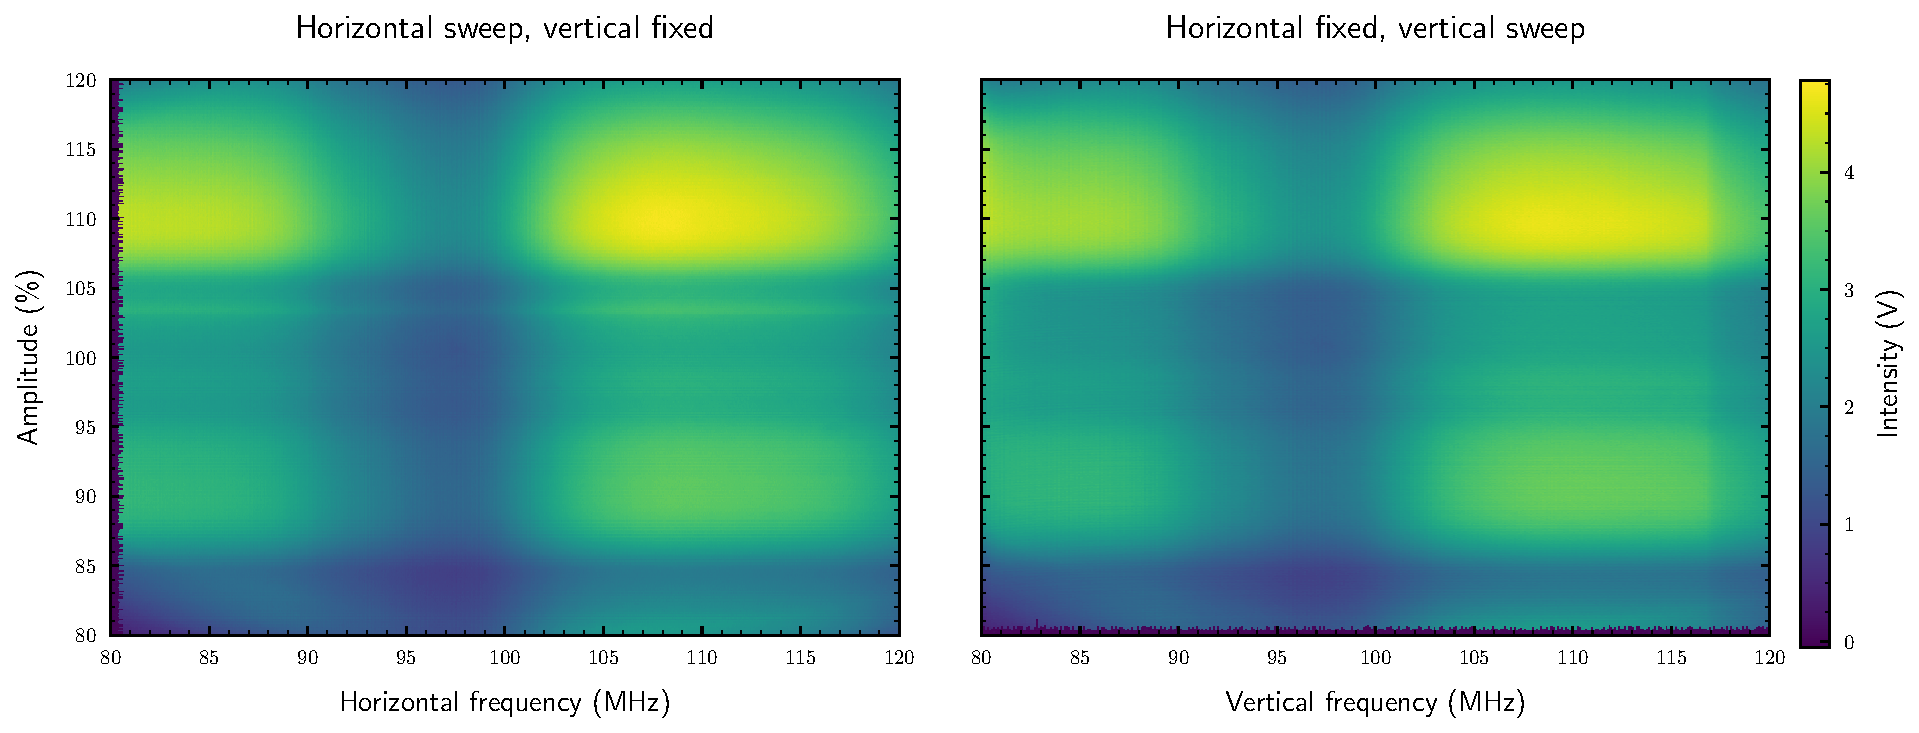
\includegraphics[width=\textwidth]{\figuredir{intensity/distribution/paired-frequency.pdf}}
  \captionsetup{width=.8\textwidth}
  \caption{Intensity measured as voltage at the photodiode in dependence of
    the horizontal and vertical applied frequency signal to the \gls{aod}. The
    left map is obtained by enabling the digital ramp on the horizontal
    \gls{dds} whereas the vertical \gls{dds} is configured to output a
    constant frequency which is manually increased after each measurement.
    On the right-hand side map the roles are exchanged.}
  \label{fig:intensity_distribution_frequency}
\end{figure}

In \Cref{fig:intensity_distribution_frequency} we are presented the intensity
measured at the second photodiode in the setup shown in
\Cref{fig:intensity_distribution_setup}. On the left-hand map the first
\gls{dds} is the \gls{dds} responsible for translations in vertical direction
whereas the second \gls{dds} is responsible for translations in horizontal
direction. This fact is also represented in the dimensionality of the
measurement data and can be observed at a close glance where we can see the
stripes in the direction of the more densely performed sweep.

\begin{figure}[h]
  \centering
  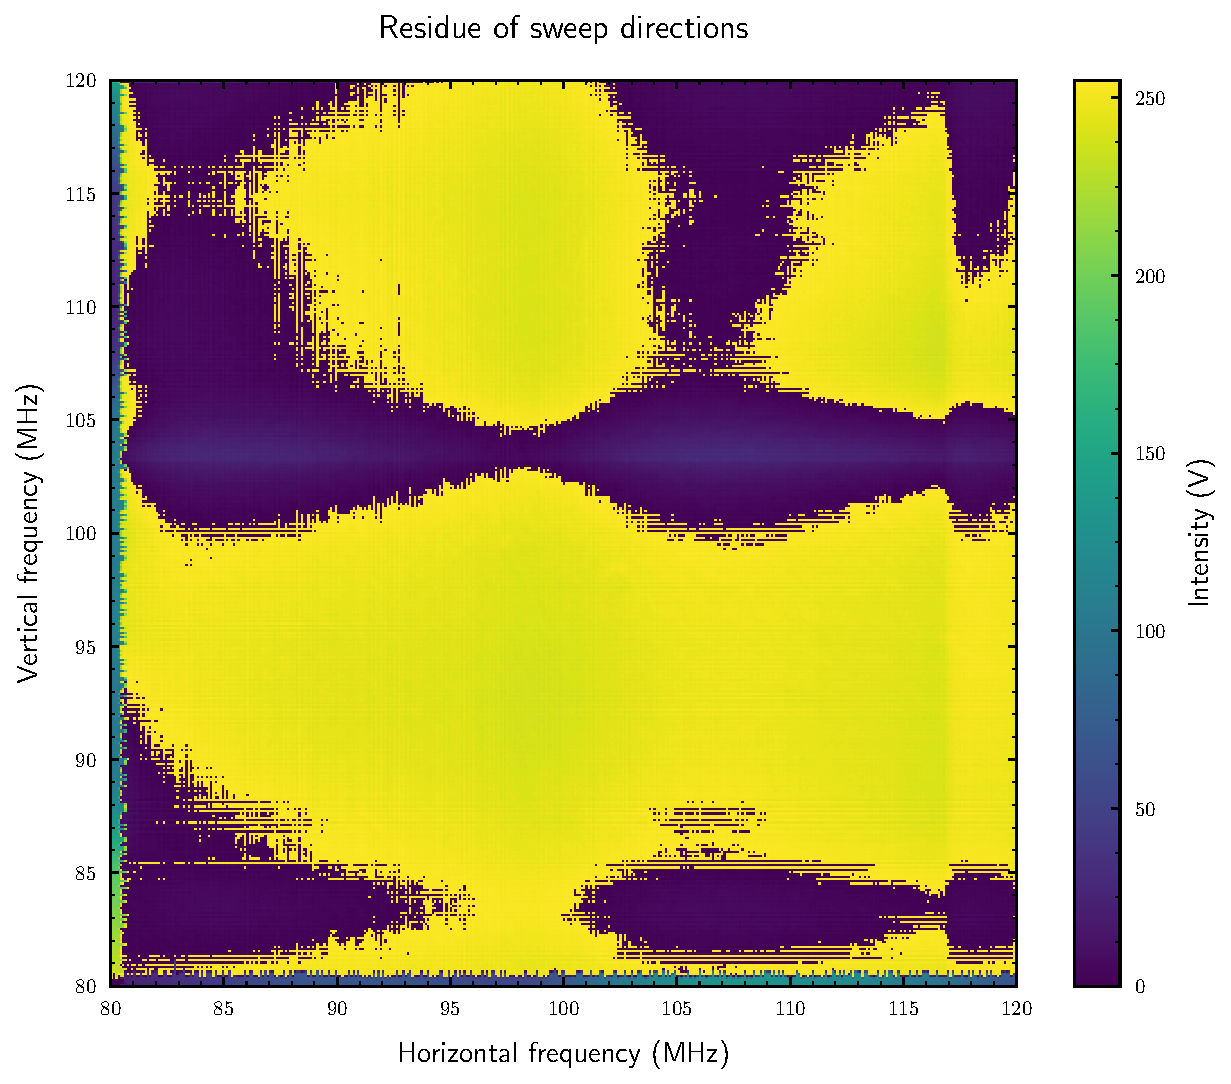
\includegraphics[width=.7\textwidth]{\figuredir{intensity/distribution/paired-frequency-residue.pdf}}
  \captionsetup{width=.9\textwidth}
  \caption{Absolute difference between the 2D intensity distribution
  performed with the digital ramp configured set to different axes.}
  \label{fig:intensity_distribution_frequency_residue}
\end{figure}

As the differences in \Cref{fig:intensity_distribution_frequency} are of only
subtile nature we additionally reveal the absolute difference between both
maps in \Cref{fig:intensity_distribution_frequency_residue}. We observe
nearly a binary map of dark purple and yellow area whereas the dark area can
be intepreted as small and the yellow area as large difference. The binary
nature of the absolute difference reminds us at the fixed offset we observed
between the amplifiers whereas the areas with small difference occur when the
crystal is saturated. However we must admit that this suggestions needs
further evidence.

\subsubsection{Constant sampled frequencies}

In \cref{subsec:signal_synthesizer_amplitude_frequency_response} we found
that the \gls{dds} show a slightly different amplitude frequency response
in the case of frequencies being controlled by the digital ramp. It remains
open if this is also true for the amplifier and in fact even more prominent.

\begin{figure}[h]
  \centering
  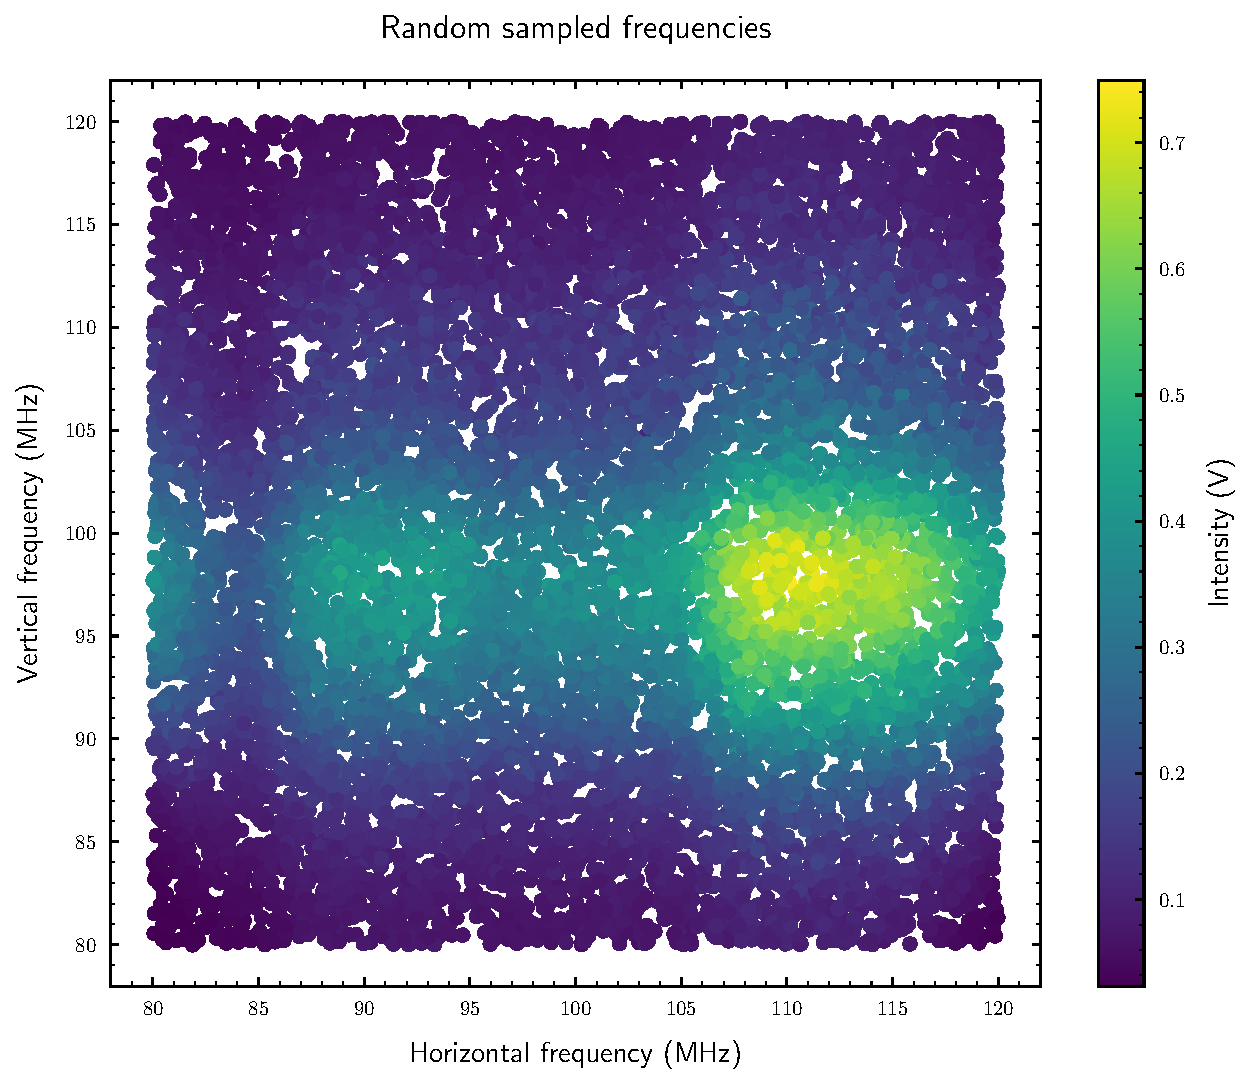
\includegraphics[width=.7\textwidth]{\figuredir{intensity/distribution/sample-frequency.pdf}}
  \captionsetup{width=.9\textwidth}
  \caption{Intensity measured as voltage at the photodiode in dependence of
    the horizontal and vertical applied frequency signal to the \gls{aod}.
    Frequency pairs are sampled over a uniform distribution and then passed
  as constant output frequency paramter to the \gls{dds}.}
  \label{fig:intensity_distribution_frequency_sampled}
\end{figure}

To partly answer this question we sampled random frequency pairs over a
two dimensional uniform distribution and passed them as constant frequency
parameter to the respective \gls{dds}. The yielded intensity distribution
is visualized in \Cref{fig:intensity_distribution_frequency_sampled}. We note
that in comparison to \Cref{fig:intensity_distribution_frequency} the
intensity differences are more concentrated around the vertical axis. This
suggests that there are electronic effects in play during fast sweeps that
do affect the intensity transmission.

\subsubsection{Different radio frequency signal source}

The previous finding suggest that the intensity transmission of the \gls{aod}
is mainly caused by unideal characteristics of the electronic equipment.
Regardless it is still unclear whether the \gls{dds} or the power amplifier
should be held responsible for messing up our signal.

For the following measurement we replaced the vertical \gls{dds} source with
a high-quality signal generator and configured a frequency sweep. We presume
the high-quality signal generator to supply a constant output power level.

\begin{figure}[h]
  \centering
  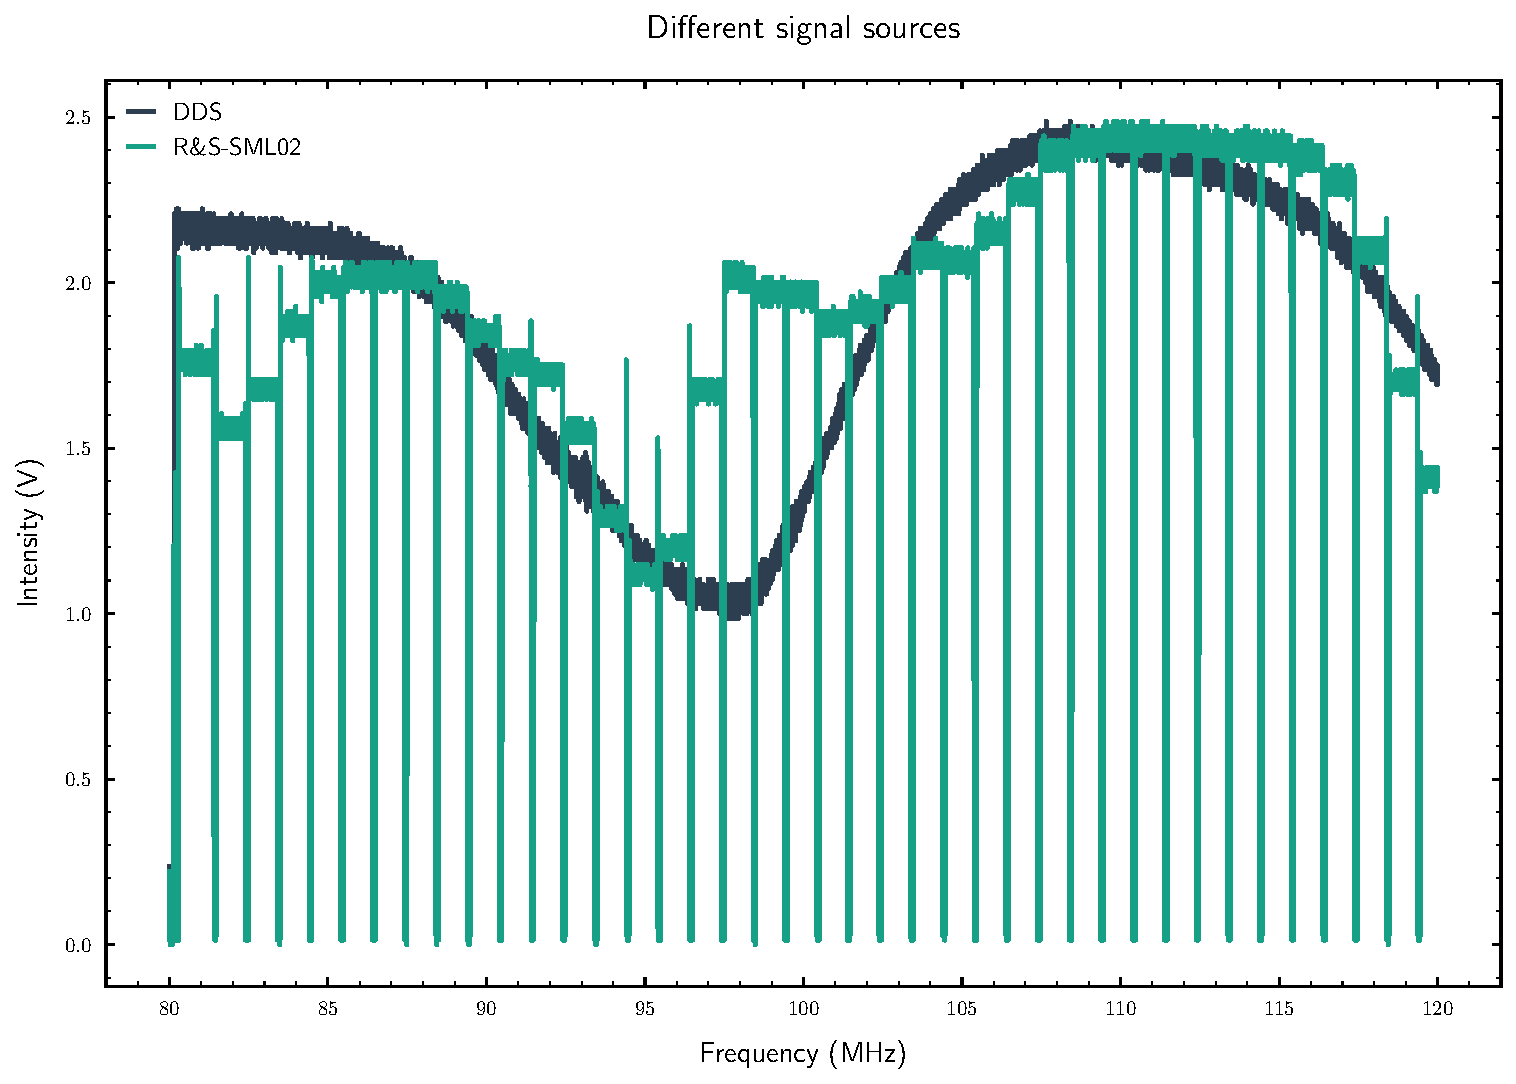
\includegraphics[width=.9\textwidth]{\figuredir{intensity/distribution/signal-sources.pdf}}
  \captionsetup{width=.9\textwidth}
  \caption{Intensity measured as voltage at the photodiode with one \gls{aod}
    at constant center frequency supplied by a \gls{dds} and the other
    \gls{aod} performing a linear frequency sweep with the \gls{dds} and a
  high-quality signal generator.}
  \label{fig:intensity_distribution_signal_sources}
\end{figure}

\Cref{fig:intensity_distribution_signal_sources} discloses the intensity
measured as voltage at the photodiode when the frequency sweep is performed
by two different signal sources and the other \gls{aod} is held at constant
center frequency. We observe that even though the signal generator has a much
more coarse frequency resolution it shares the global characteristics of
the more dense trace from the \gls{dds}. This confirms that the amplifier
seems to be the dominant contributor to the intensity transmission during
frequency sweeps.

\subsubsection{Summary}

In this chapter we found out that the \gls{rf} signal is of major importance
to the observed intensity transmission. In particular the power amplifier
possess a strong frequency power response. The acousto-optics itself seem to
be saturated at some power level. Transmission also seems to differ depending
on the method used to sweep frequencies. All in all there are to many factors
at play to describe with a simple analytical model and we will further try to
not expect much regularities for the optimization procedure in the next
chapter.

\chapter{Acousto-optic intensity optimization}

The previous two chapters addressed the characteristics of the \gls{rf}
signal and the intensity transmission of the \gls{aod}. Therewith the
groundwork has been set out to finally approach the mission of minimizing the
intensity variance to obtain a homogenous optical potential.

But how do we minimize the intensity variance? The \gls{dds} permit to read
$N=1024$ amplitude values from memory. The optimization problem therefore is to
minimize the variance of the intensity distribution $I(A)$ subject to an
amplitude vector $A\in[0,1]^N$. The conclusions drawn from the intensity
measurements suggest that we have to expect non-linear, irregular behaviour
in $I(A)$. and indeed first attempts to model $I(A)$ through polynomial fits,
multilayer perceptron networks and least-squared minimizations have failed.

During these optimization procedures we observed that changing an amplitude
value $A_i\in A$ does affect the intensity voltage at subsequent
$A_{i+1},\dots,A_N$. Fortunately we found that by respecting the amplitude
order with respect to increasing frequency during optimization we where able
to bypass these effects. Further we created amplitude segments
$\left(A_j,\dots,A_{j+m}\right)$ consisting of $m$ ordered amplitude values
to reduce the optimization time. Optimization then was performed through
random search which was proven to yield better results as grid search
\cite{Bergstra2012}.

\subsubsection{Overview}

First of we want to provide an overview of the final optimization results
obtained at different hyperparameters for the random search. The
hyperparameter include the number of amplitude segments $N/m$ and the target
intensity.

\begin{figure}[h]
  \centering
  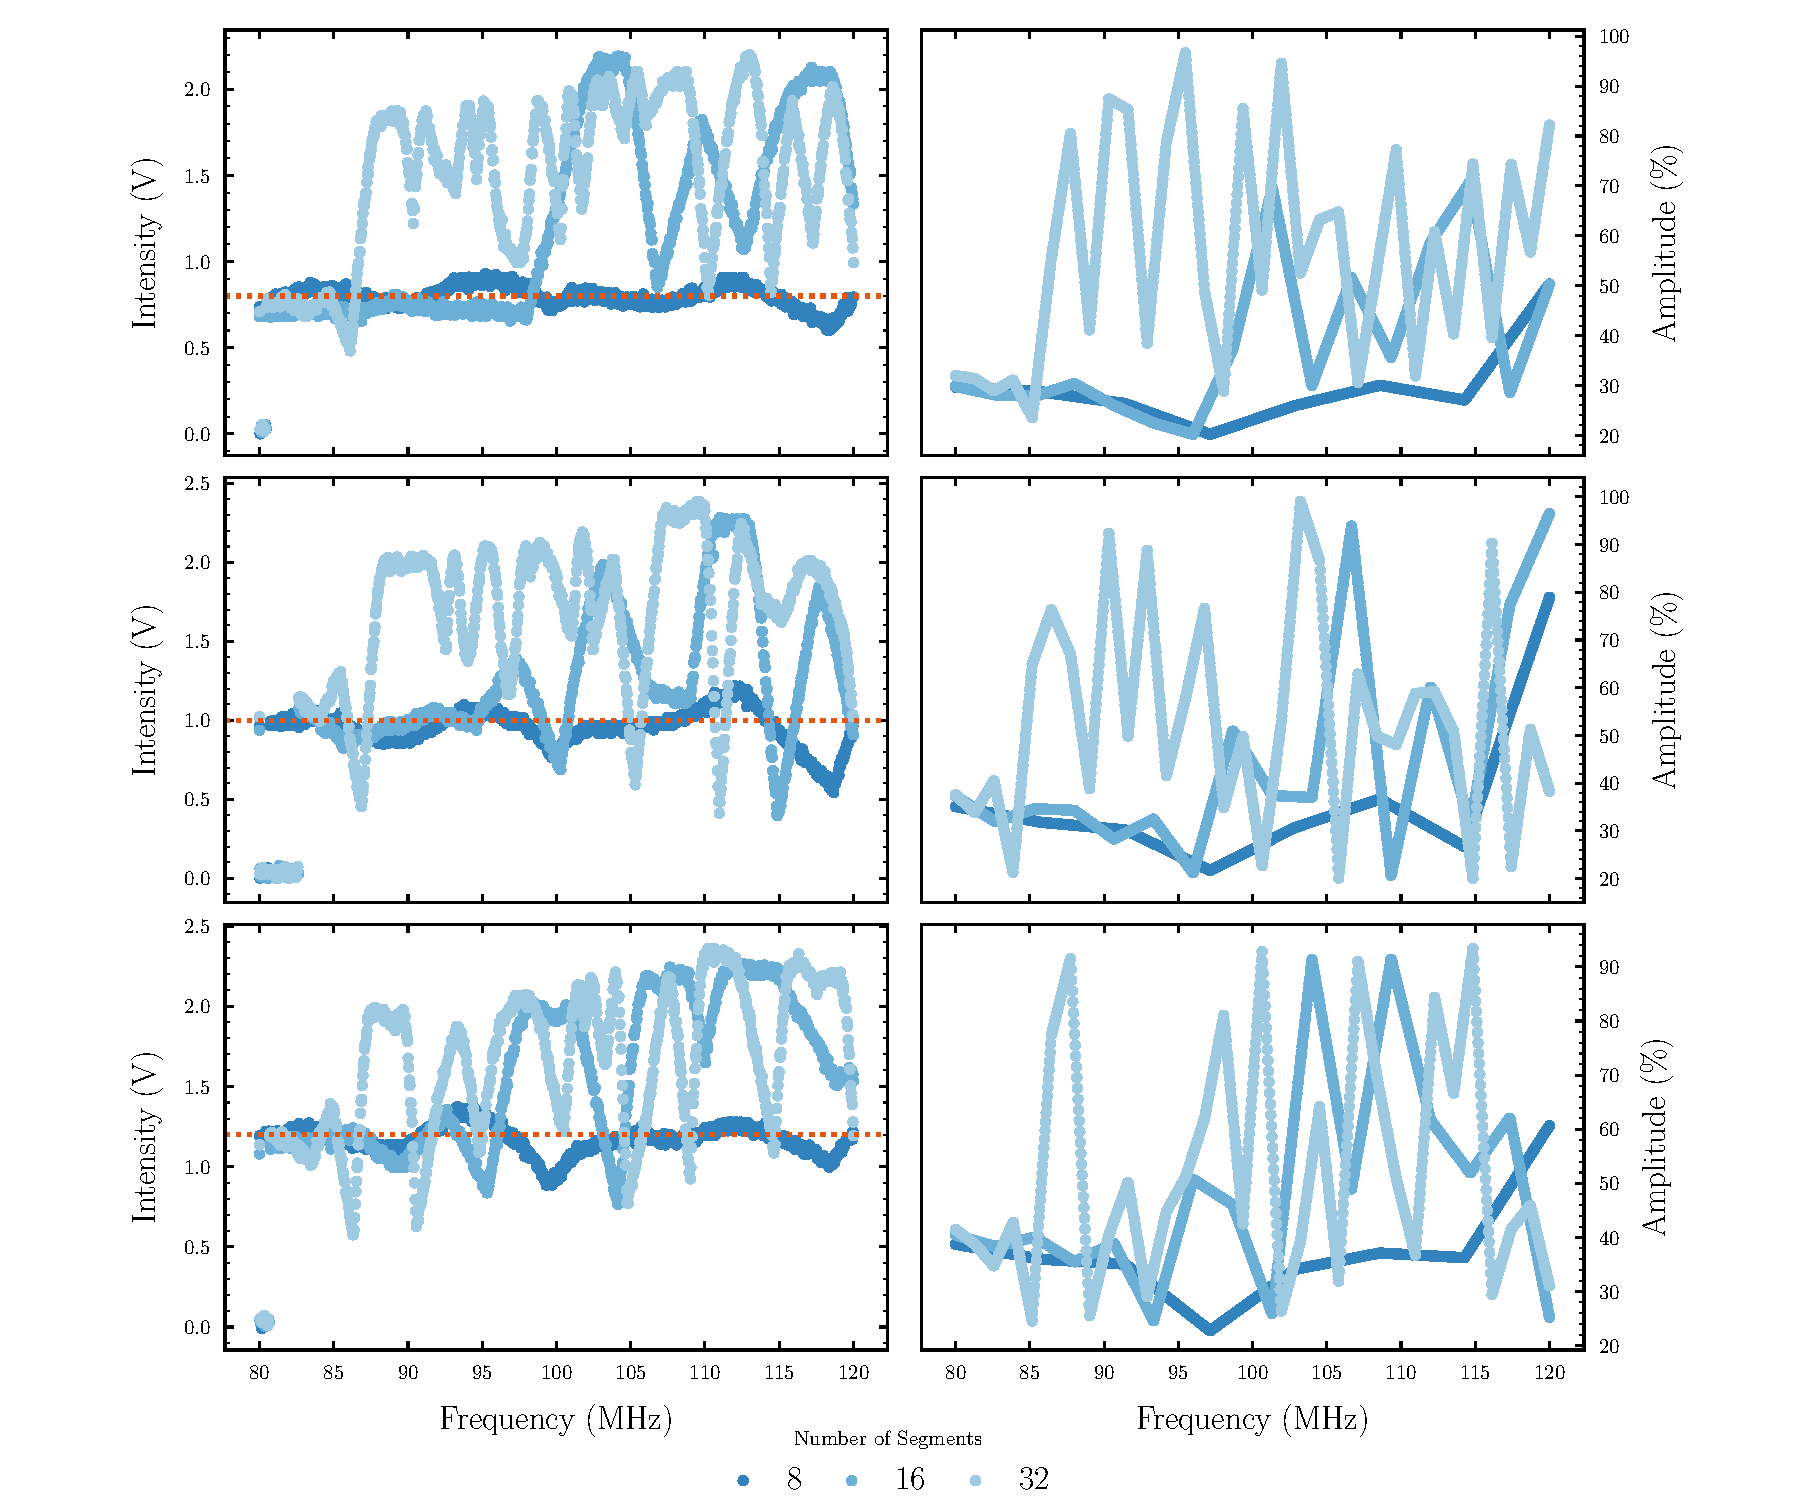
\includegraphics[width=\textwidth]{\figuredir{intensity/optimization/overview.pdf}}
  \captionsetup{width=.8\textwidth}
  \caption{Minimized intensity variance for different target intensities
  and number of amplitude segments. We note heavy oscillations for
  amplitude segments greater than eight.}
  \label{fig:intensity_optimization_overview}
\end{figure}

In \Cref{fig:intensity_optimization_overview} we are presented the final
optimization results for target intensities of \SI{800}{\milli\volt},
\SI{1000}{\milli\volt} and \SI{1200}{\milli\volt} and amplitude segments
$8,16,32$. We observe heavy oscillations for amplitude segments greater than
eight. The optimization results using 16 amplitude segments performs better
than the run with 32 amplitude segments.

We assume that inductive effects occur when choosing more amplitude segments
that consolidate a non-linear intensity response. For the sake of simplicity
we will first limit us to the case of eight amplitude segments.

\begin{figure}[h]
  \centering
  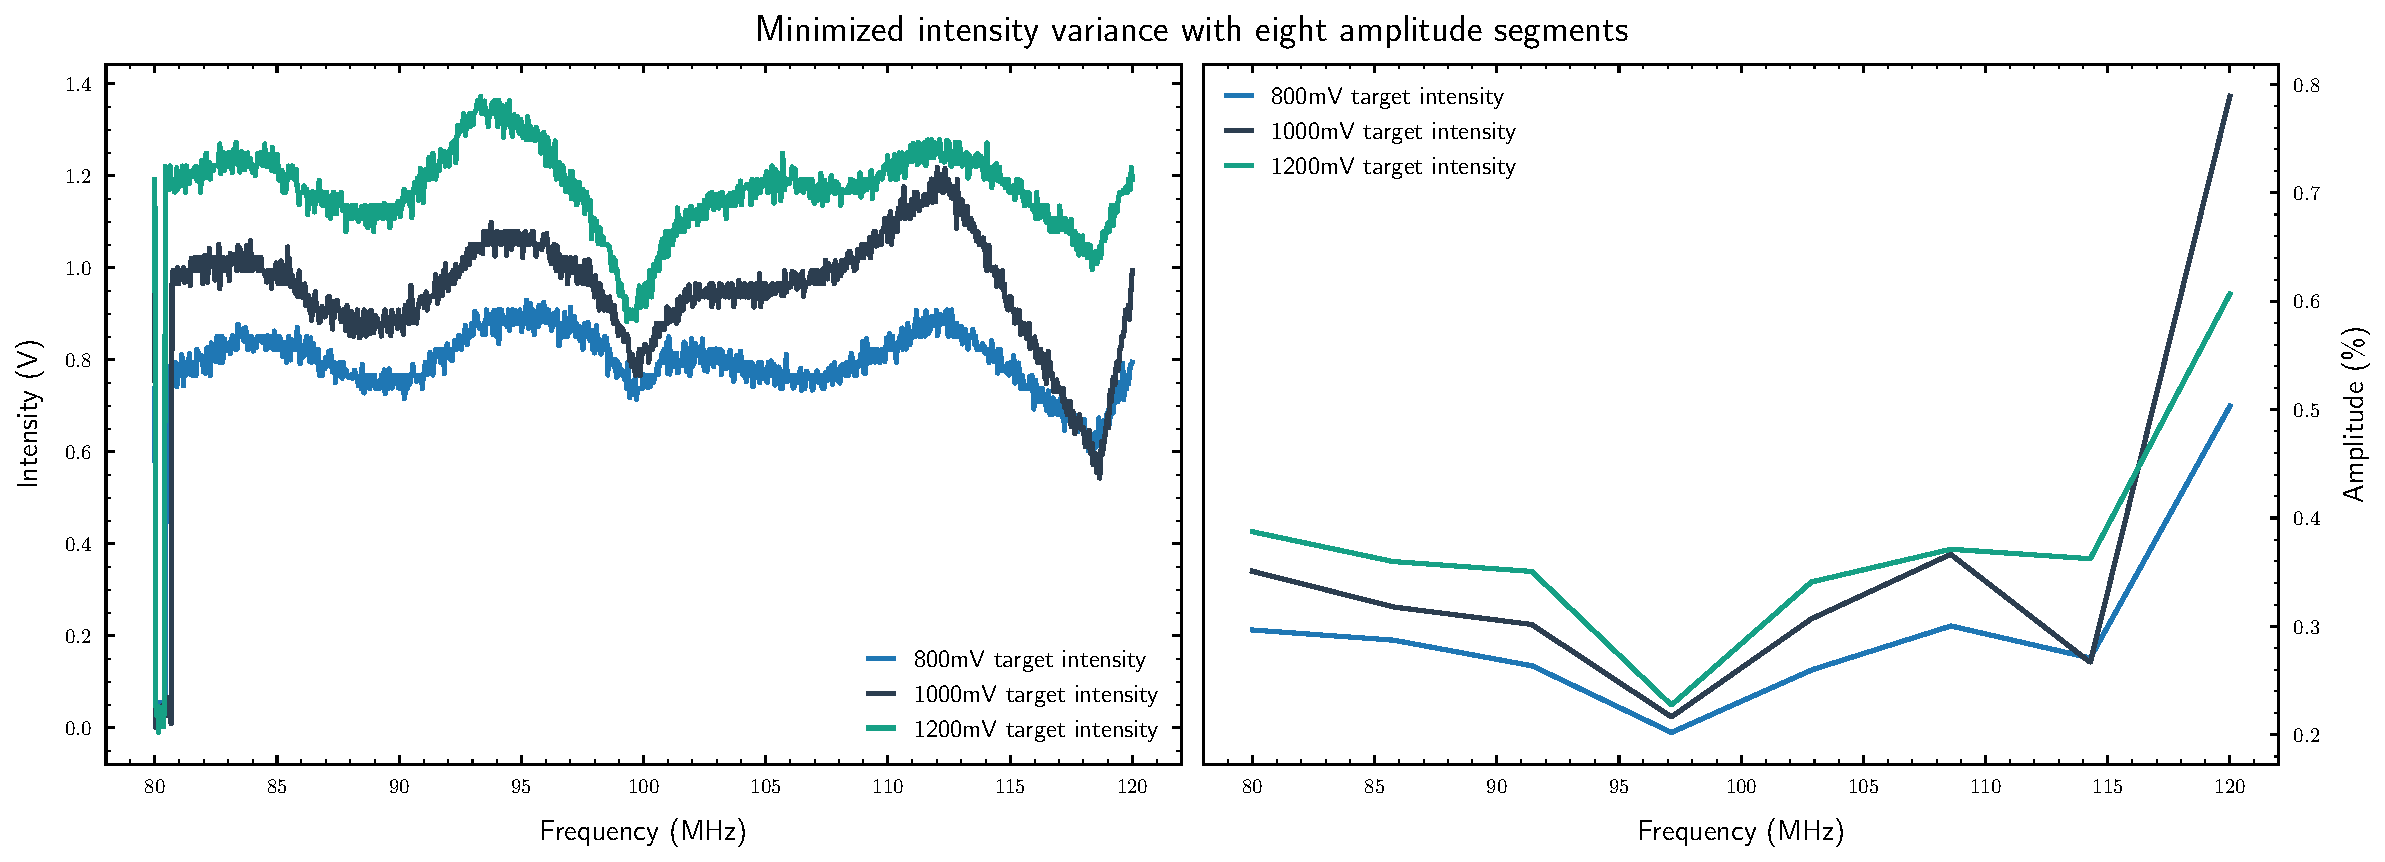
\includegraphics[width=\textwidth]{\figuredir{intensity/optimization/intensity-amplitude.pdf}}
  \captionsetup{width=.8\textwidth}
  \caption{Final result of the intensity variance minimization and the
  corresponding amplitude segment values obtained through random search with
  eight independent amplitude segments.}
  \label{fig:intensity_optimization_intensity_amplitude}
\end{figure}

In \Cref{fig:intensity_optimization_intensity_amplitude} we have a closer
view on the first column of \Cref{fig:intensity_optimization_overview}. We
can notice similar characteristics observed in the \gls{rf} signal. In
particular the more power drop near the center frequency is present and the
linear power fall off with the frequency in the second half of the frequency
sweep.

\subsubsection{Process}

We now want to elaborate on the optimization process. We limit ourselves to
the optimization process with eight amplitude segments as it was the most
successful one and can be covered completly with eight plots.

\begin{figure}[h]
  \centering
  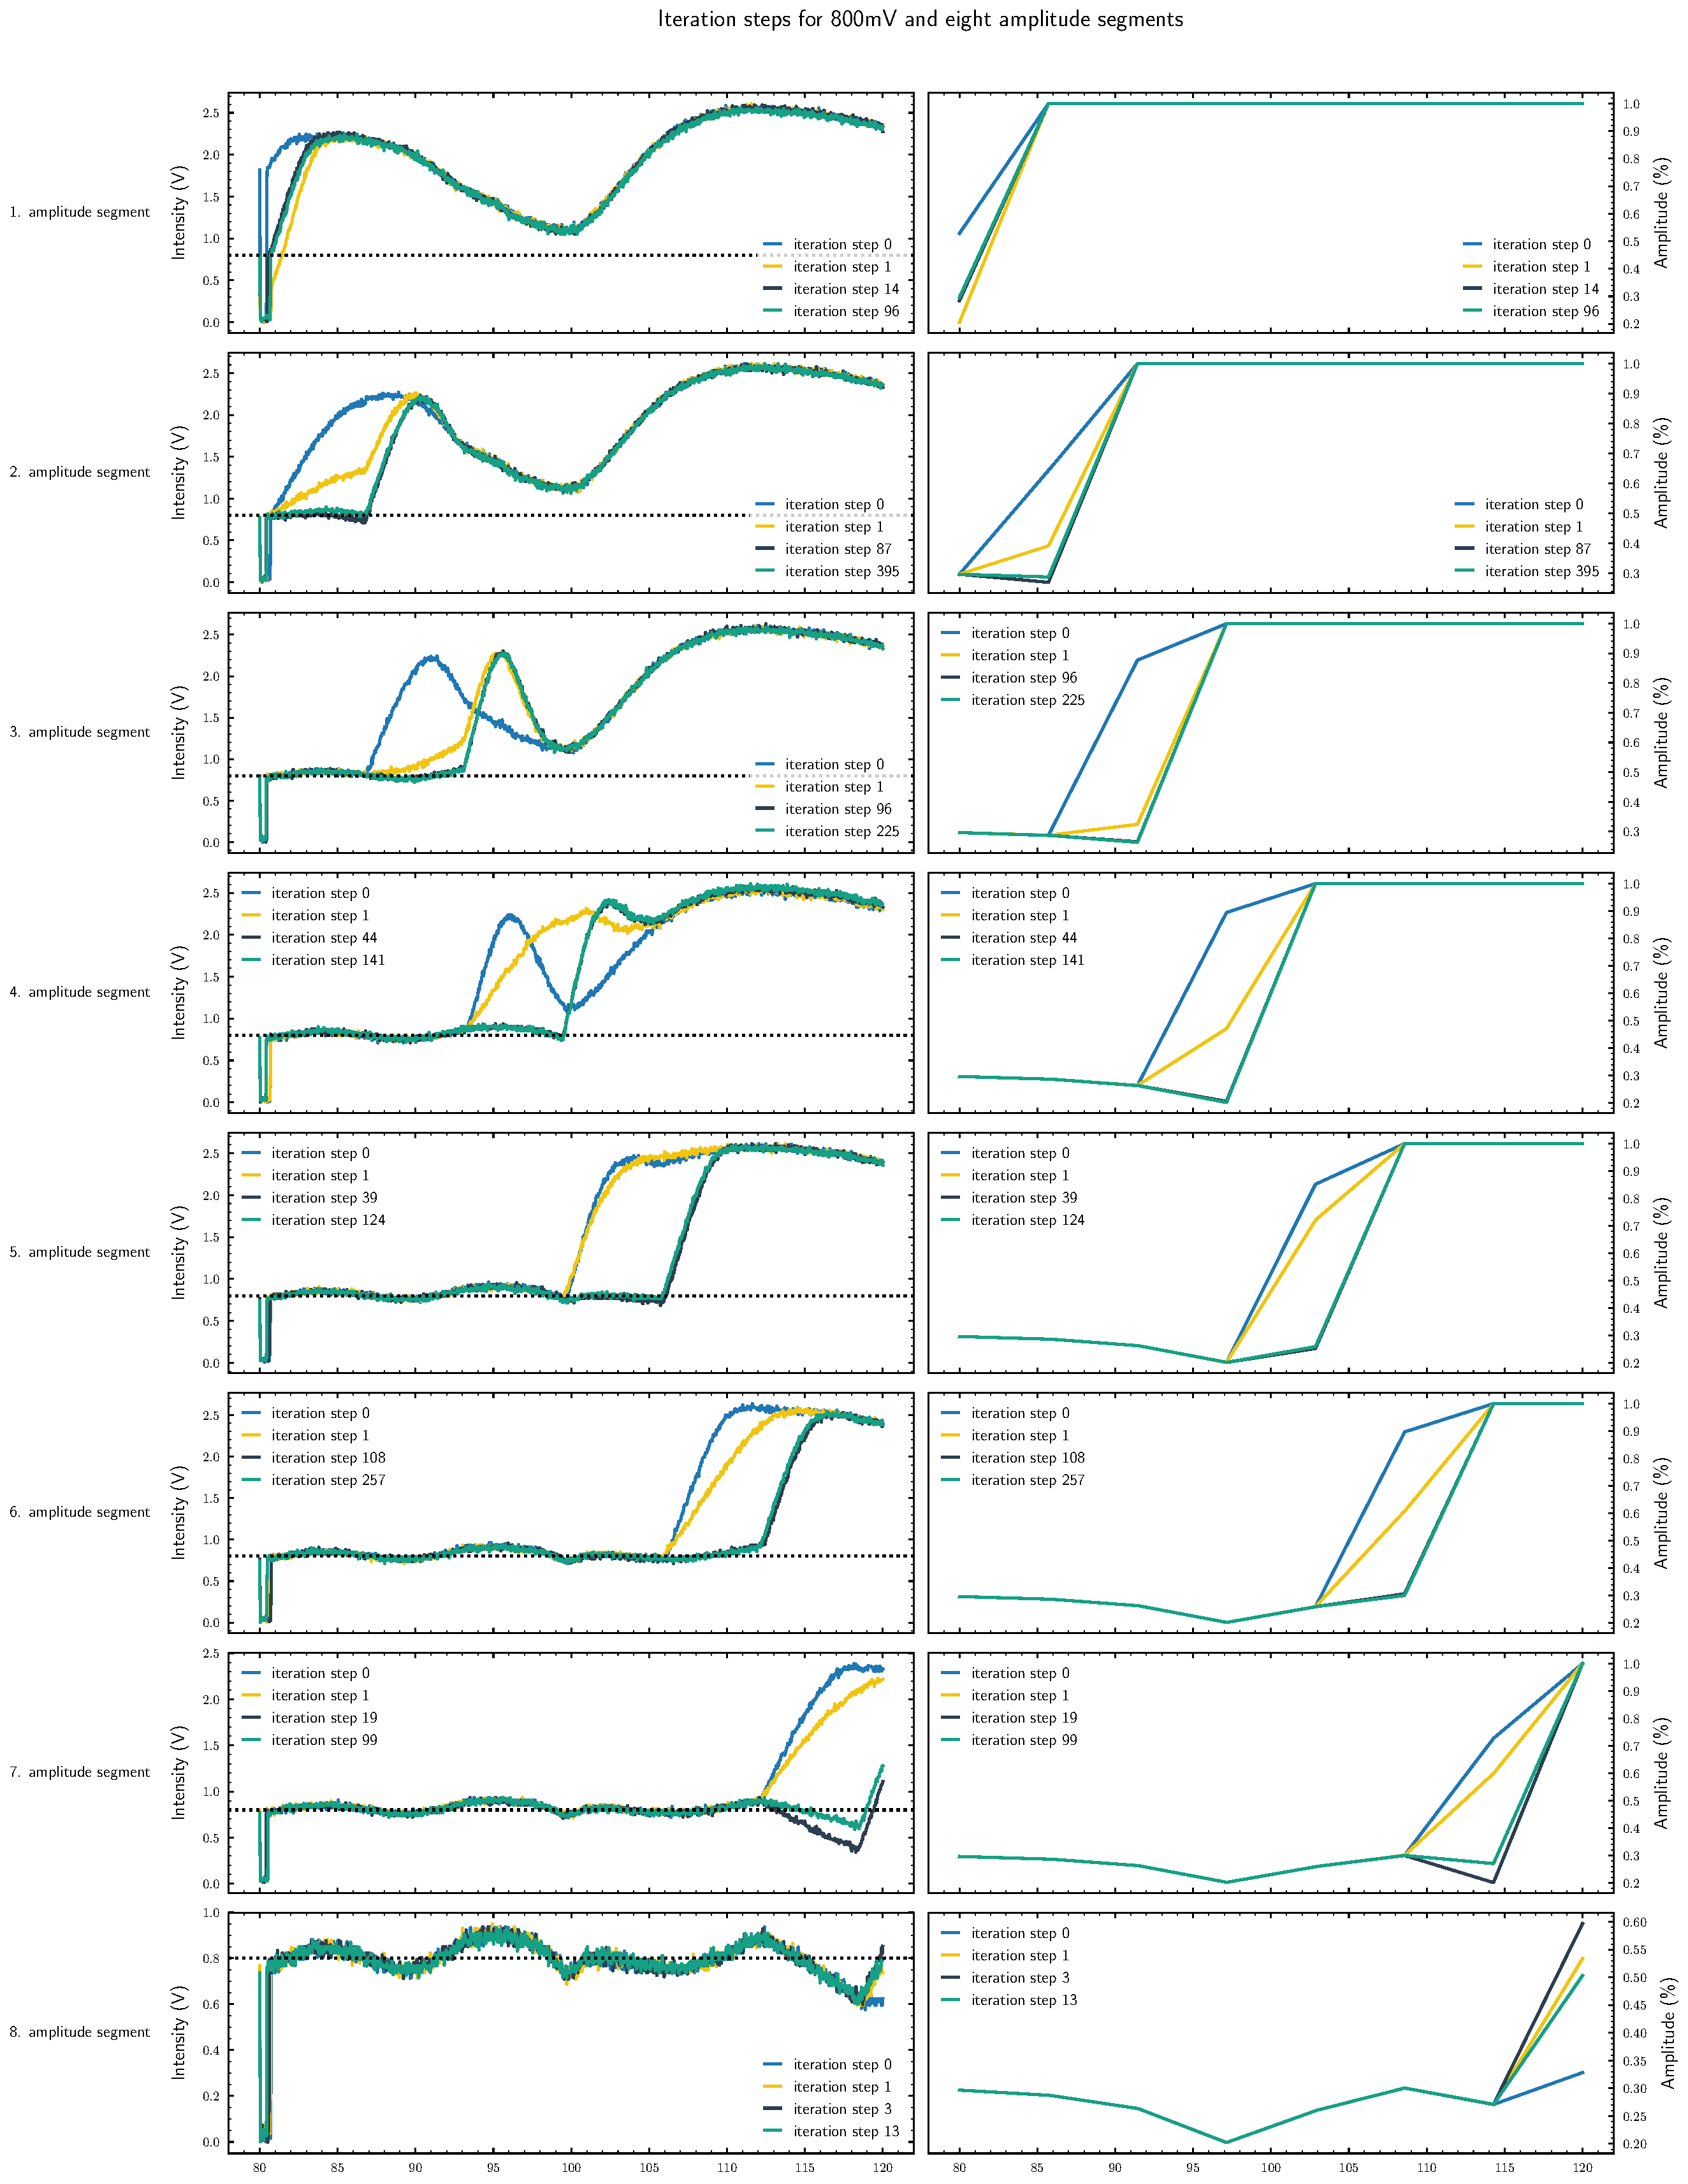
\includegraphics[width=\textwidth]{\figuredir{intensity/optimization/process.pdf}}
  \captionsetup{width=.8\textwidth}
  \caption{Intensity and amplitude at different stages of the optimization
  process. In each column a different amplitude segment is optimized.
  The different traces in each plot mark the respective iteration.}
  \label{fig:intensity_optimization_process}
\end{figure}

In \Cref{fig:intensity_optimization_process} we see the intensity and
amplitude at different optimization stages. At each stage one amplitude
segment is sampled from a uniform distribution over $[.2, .8]$. The intensity
segment associated with this amplitude segment is then used to calculate
the \gls{mse} and compare it to the previous best \gls{mse}. If the new
\gls{mse} is less than the previous best \gls{mse} the previous best \gls{mse}
is updated and the amplitude segment value is saved. This procedure is
repeated 500 times. Every time a new best value was found we saved the
data. For the diagrams we choose the four most separated iteration steps to
visualize the process of the optimization.

If we take a look at the succeeding segment from the currently optimized
amplitude segment we observe that these differ for different amplitude
values and henceforth confirms that amplitude values are not independent but
affect subsequent segments.

\subsubsection{Failure}

With the optimization showing reasonable convergence for eight amplitude
segments we would expect it to improve if we choose a more amplitude segments,
yet we observed heavy oscillations. In this section we want to check the
optimization process in the case of 32 amplitude segments to investigate in
possible origins of the optimization failure.

\begin{figure}[h]
  \centering
  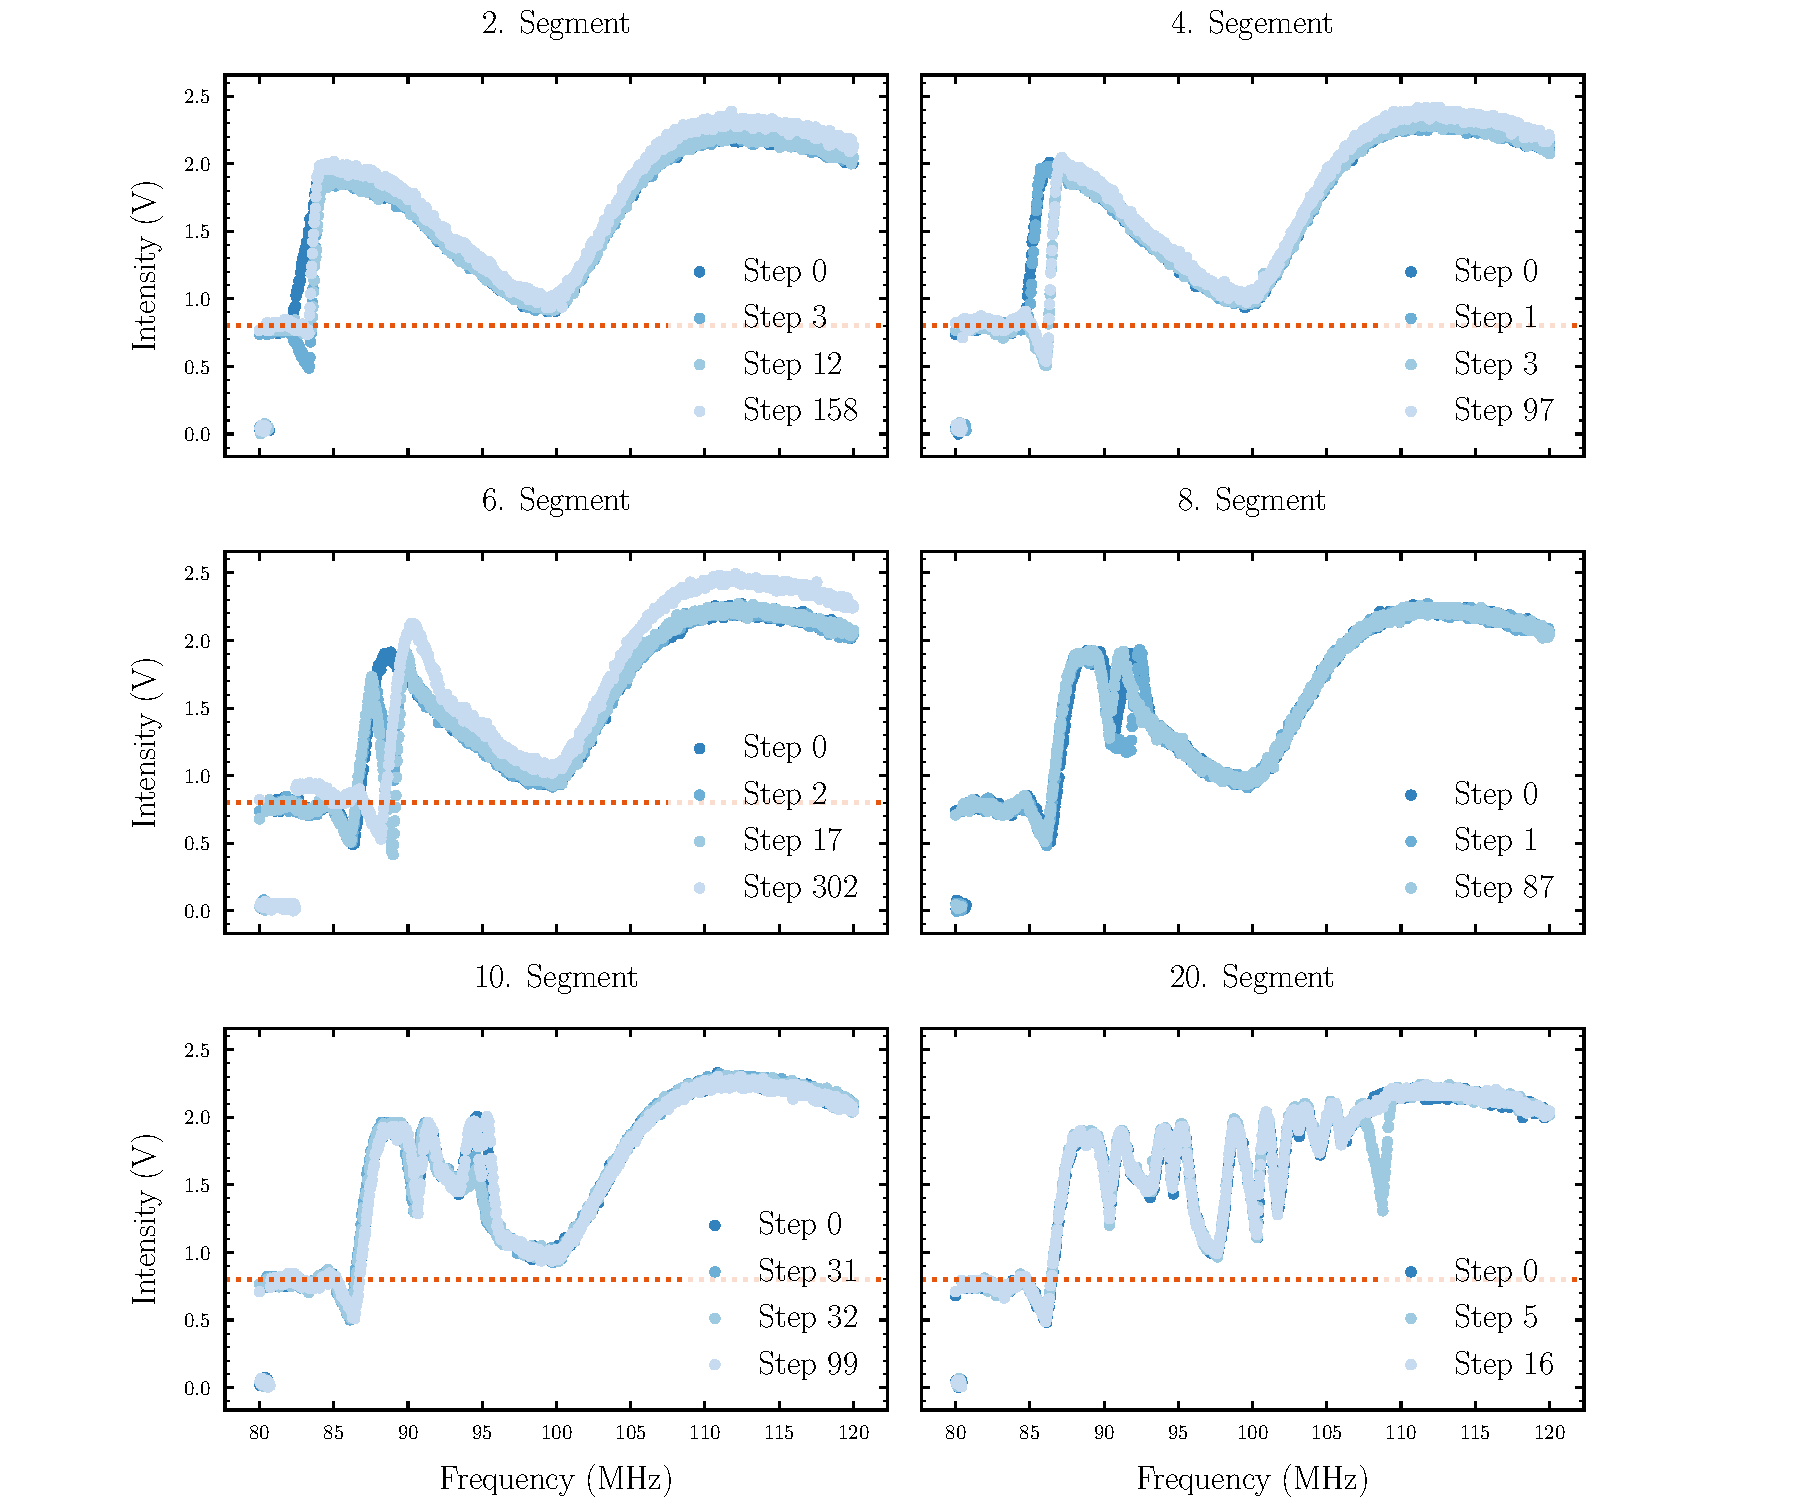
\includegraphics[width=\textwidth]{\figuredir{intensity/optimization/failure.pdf}}
  \captionsetup{width=.8\textwidth}
  \caption{Optimization progress for the 2.,4.,6.,8.,10. and 20. amplitude
  segment of the failed optimization run with 32 amplitude segments. We can
  see that with increasing amplitude segments the non-linear response
  following the optimized amplitude segment increases.}
  \label{fig:intensity_optimization_failure}
\end{figure}

In \Cref{fig:intensity_optimization_failure} we can see the optimization
progress for selected amplitude segments of the optimization run with 32
segments. We observe that with the non-linear response following the actual
optimized amplitude segment increases more and more.

\subsubsection{Summary}

Our attemps to minimize the intensity variance where of mixed success. One
the one hand side we were able to minimize the intensity deviation down
to \SI{100}{\milli\volt} on the other hand we were not able to train any
model on the intensity response that would allow fast optimization or even
predicition of the expected intensity response given an amplitude
configuration.

However we also found out that irregularities arise with increase in the
number of amplitude segments. We suspect that fast changes of the output
amplitude draws power that may non deterministicyl affect the next clock
cycle inside the \gls{dds}. Given that the one dimensional optimizations
already required multiple hours to run and the non-linear response between
amplitude segments we do not believe that it is not in the capabilites of the
\gls{dds} to compensate for the two dimensional intensity distribution
measured in the previous chapter.

\chapter{Conclusion}

\section{Summary}

\section{Future Outlook}

\section{Further Applications}


\printglossaries
\listoffigures
\listoftables
\listoflistings
\printbibliography

\appendix
\chapter{Electronics}

\section{Trigger Hub}
\label{app:electronics:trigger_hub}

The trigger hub is driven by a \SI{3.3}{\volt} input signal and a
\SI{5}{\volt} voltage source. The input signal is amplified to drive four
\gls{ttl} inputs through use of the \gls{sn74128} \cite{SN74128} line driver.
Furthermore the hub is designed to be mounted on the \gls{bbb} which itself
provides the trigger network interface.

\begin{figure}[h]
  \centering
  \captionsetup{width=.8\textwidth}
  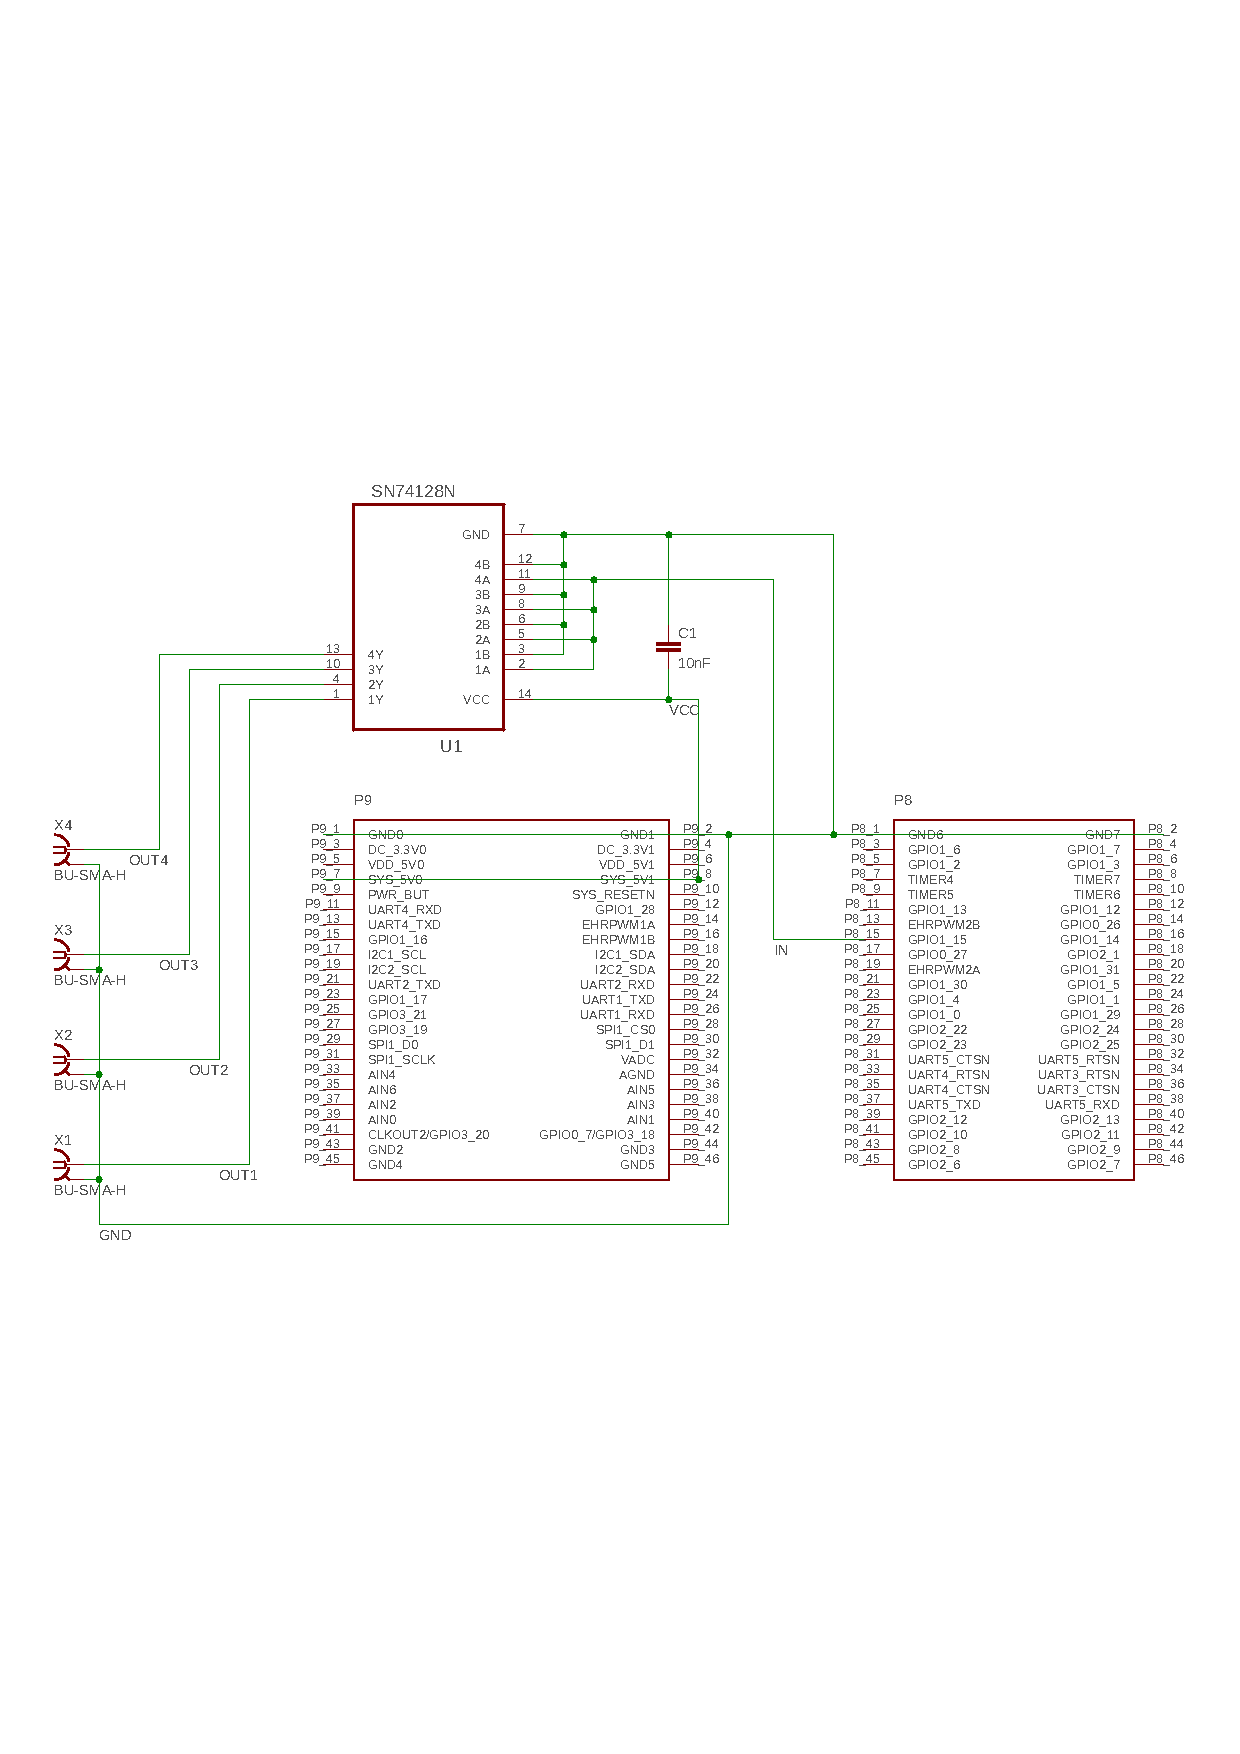
\includegraphics[width=\textwidth]{images/circuits/line-driver/schematic.pdf}
  \caption{Elecronic circuit schematics of the trigger hub. The
    \SI{3.3}{\volt} input signal is amplified by the \gls{sn74128} line
    driver and outputed to four \gls{sma} connectors.}
\end{figure}

The \gls{sn74128} exposes four independent outputs $Y$, each is driven by a
two-input ($A$ and $B$) with NOR ($\overline{A+B}=Y$) logic. As our objective
is to forward rising edge trigger signals we pulled all four $B$ to low by
connecting them with \gls{gnd}. The four $A$ where connected together with
the input signal. The input signal has to transition from $1$ to $0$ in order
to signal a rising edge trigger signal.

\begin{listing}[h]
  \inputminted[xleftmargin=.2\linewidth]{javascript}{scripts/trigger.js}
  \captionsetup{width=.6\linewidth}
  \caption{\gls{bbb} script that starts a \gls{http} server to listen for
requests on which to trigger a rising edge signal. On execution it pulls the
signal \gls{gpio} to high. The request callback then pulls the \gls{gpio} to
low for one \SI{1}{\milli\second}.}
\end{listing}

Using the \gls{bbb} makes it easy to write scripts that communicate with
other devices over the \gls{lan}. We used the bonescript library to access
the \gls{gpio} interface as it is pre-installed on the \gls{bbb}.

\begin{figure}[h]
  \centering
  \begin{minipage}{.40\textwidth}
    \centering
    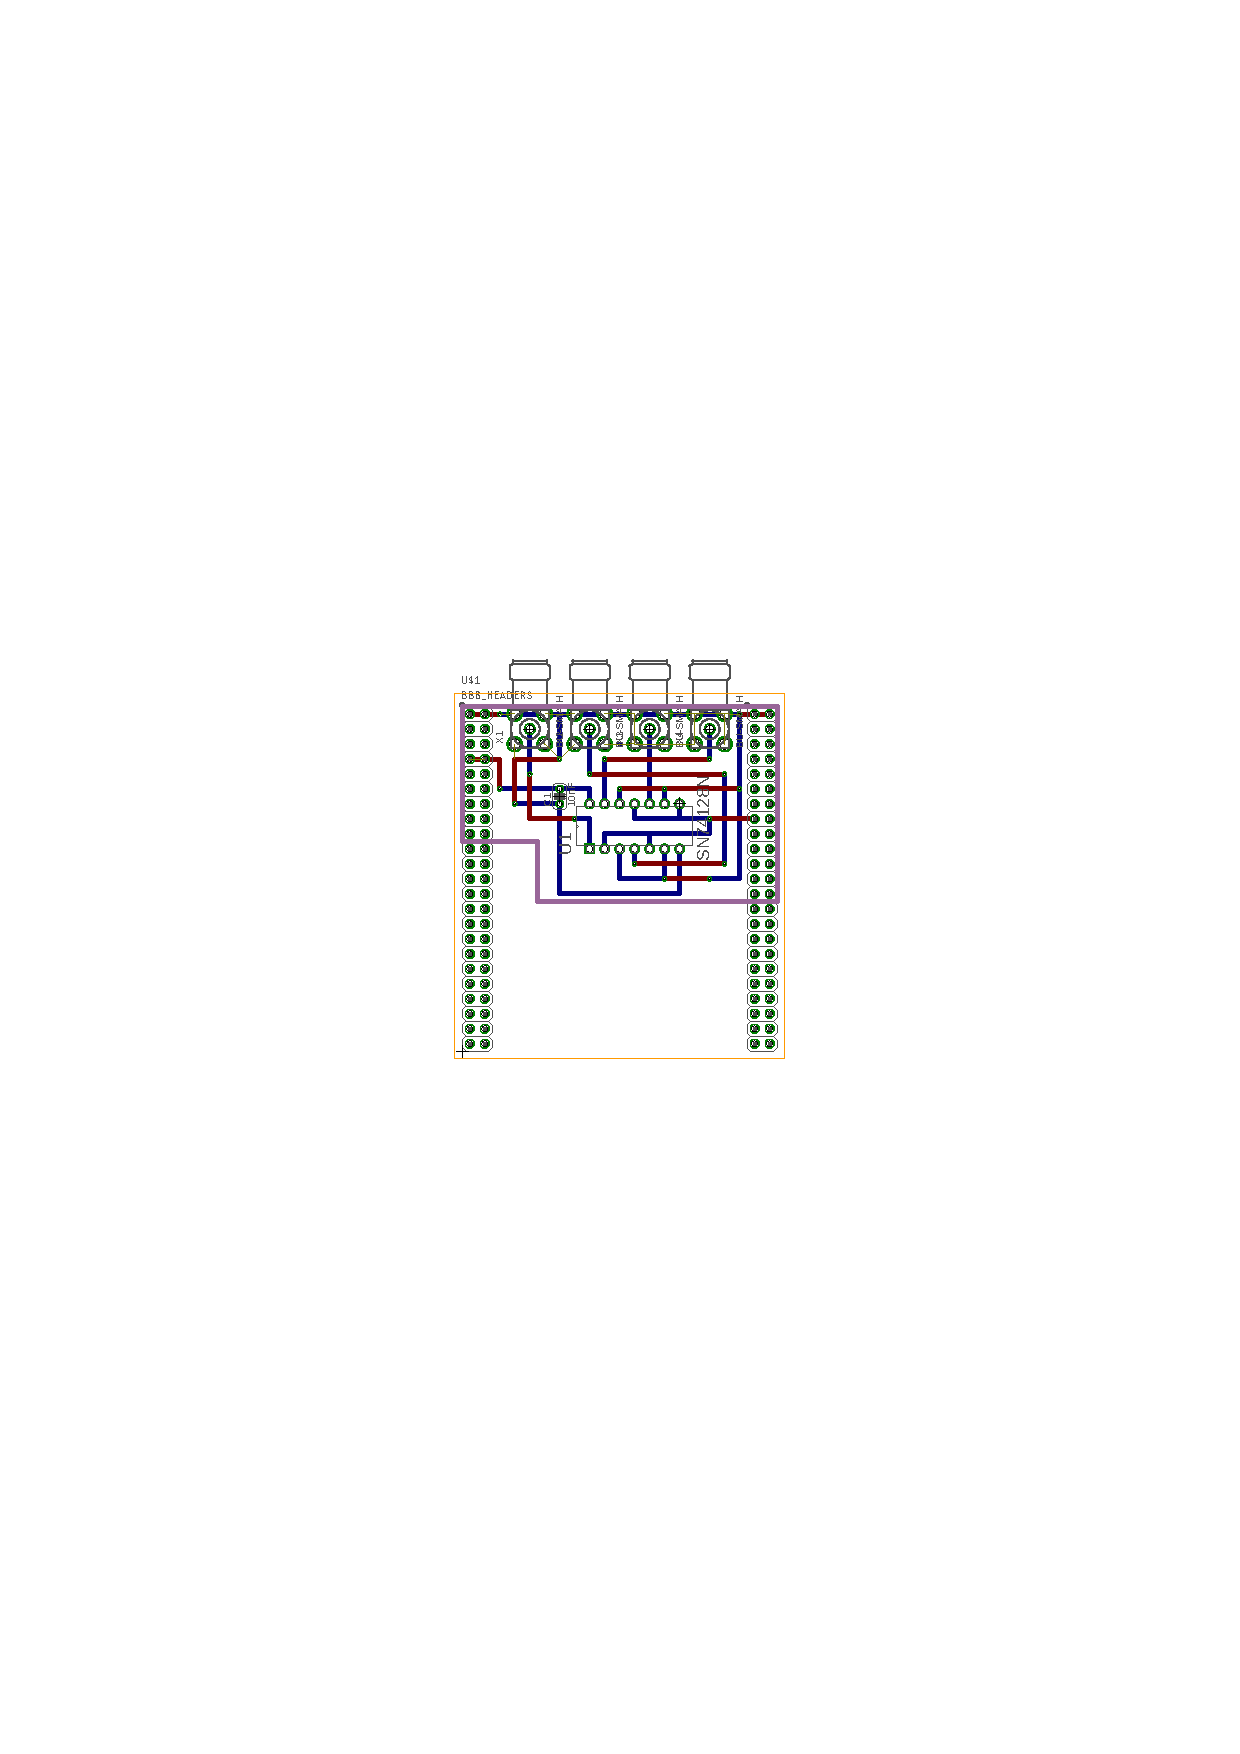
\includegraphics[width=\linewidth]{images/circuits/line-driver/layout.pdf}
    \captionsetup{width=\linewidth}
    \caption{Board layout of the trigger hub. The source amplifier is designed
to fit on top of the \gls{bbb} expansion headers.}
  \end{minipage}
  \begin{minipage}{.50\textwidth}
    \centering
    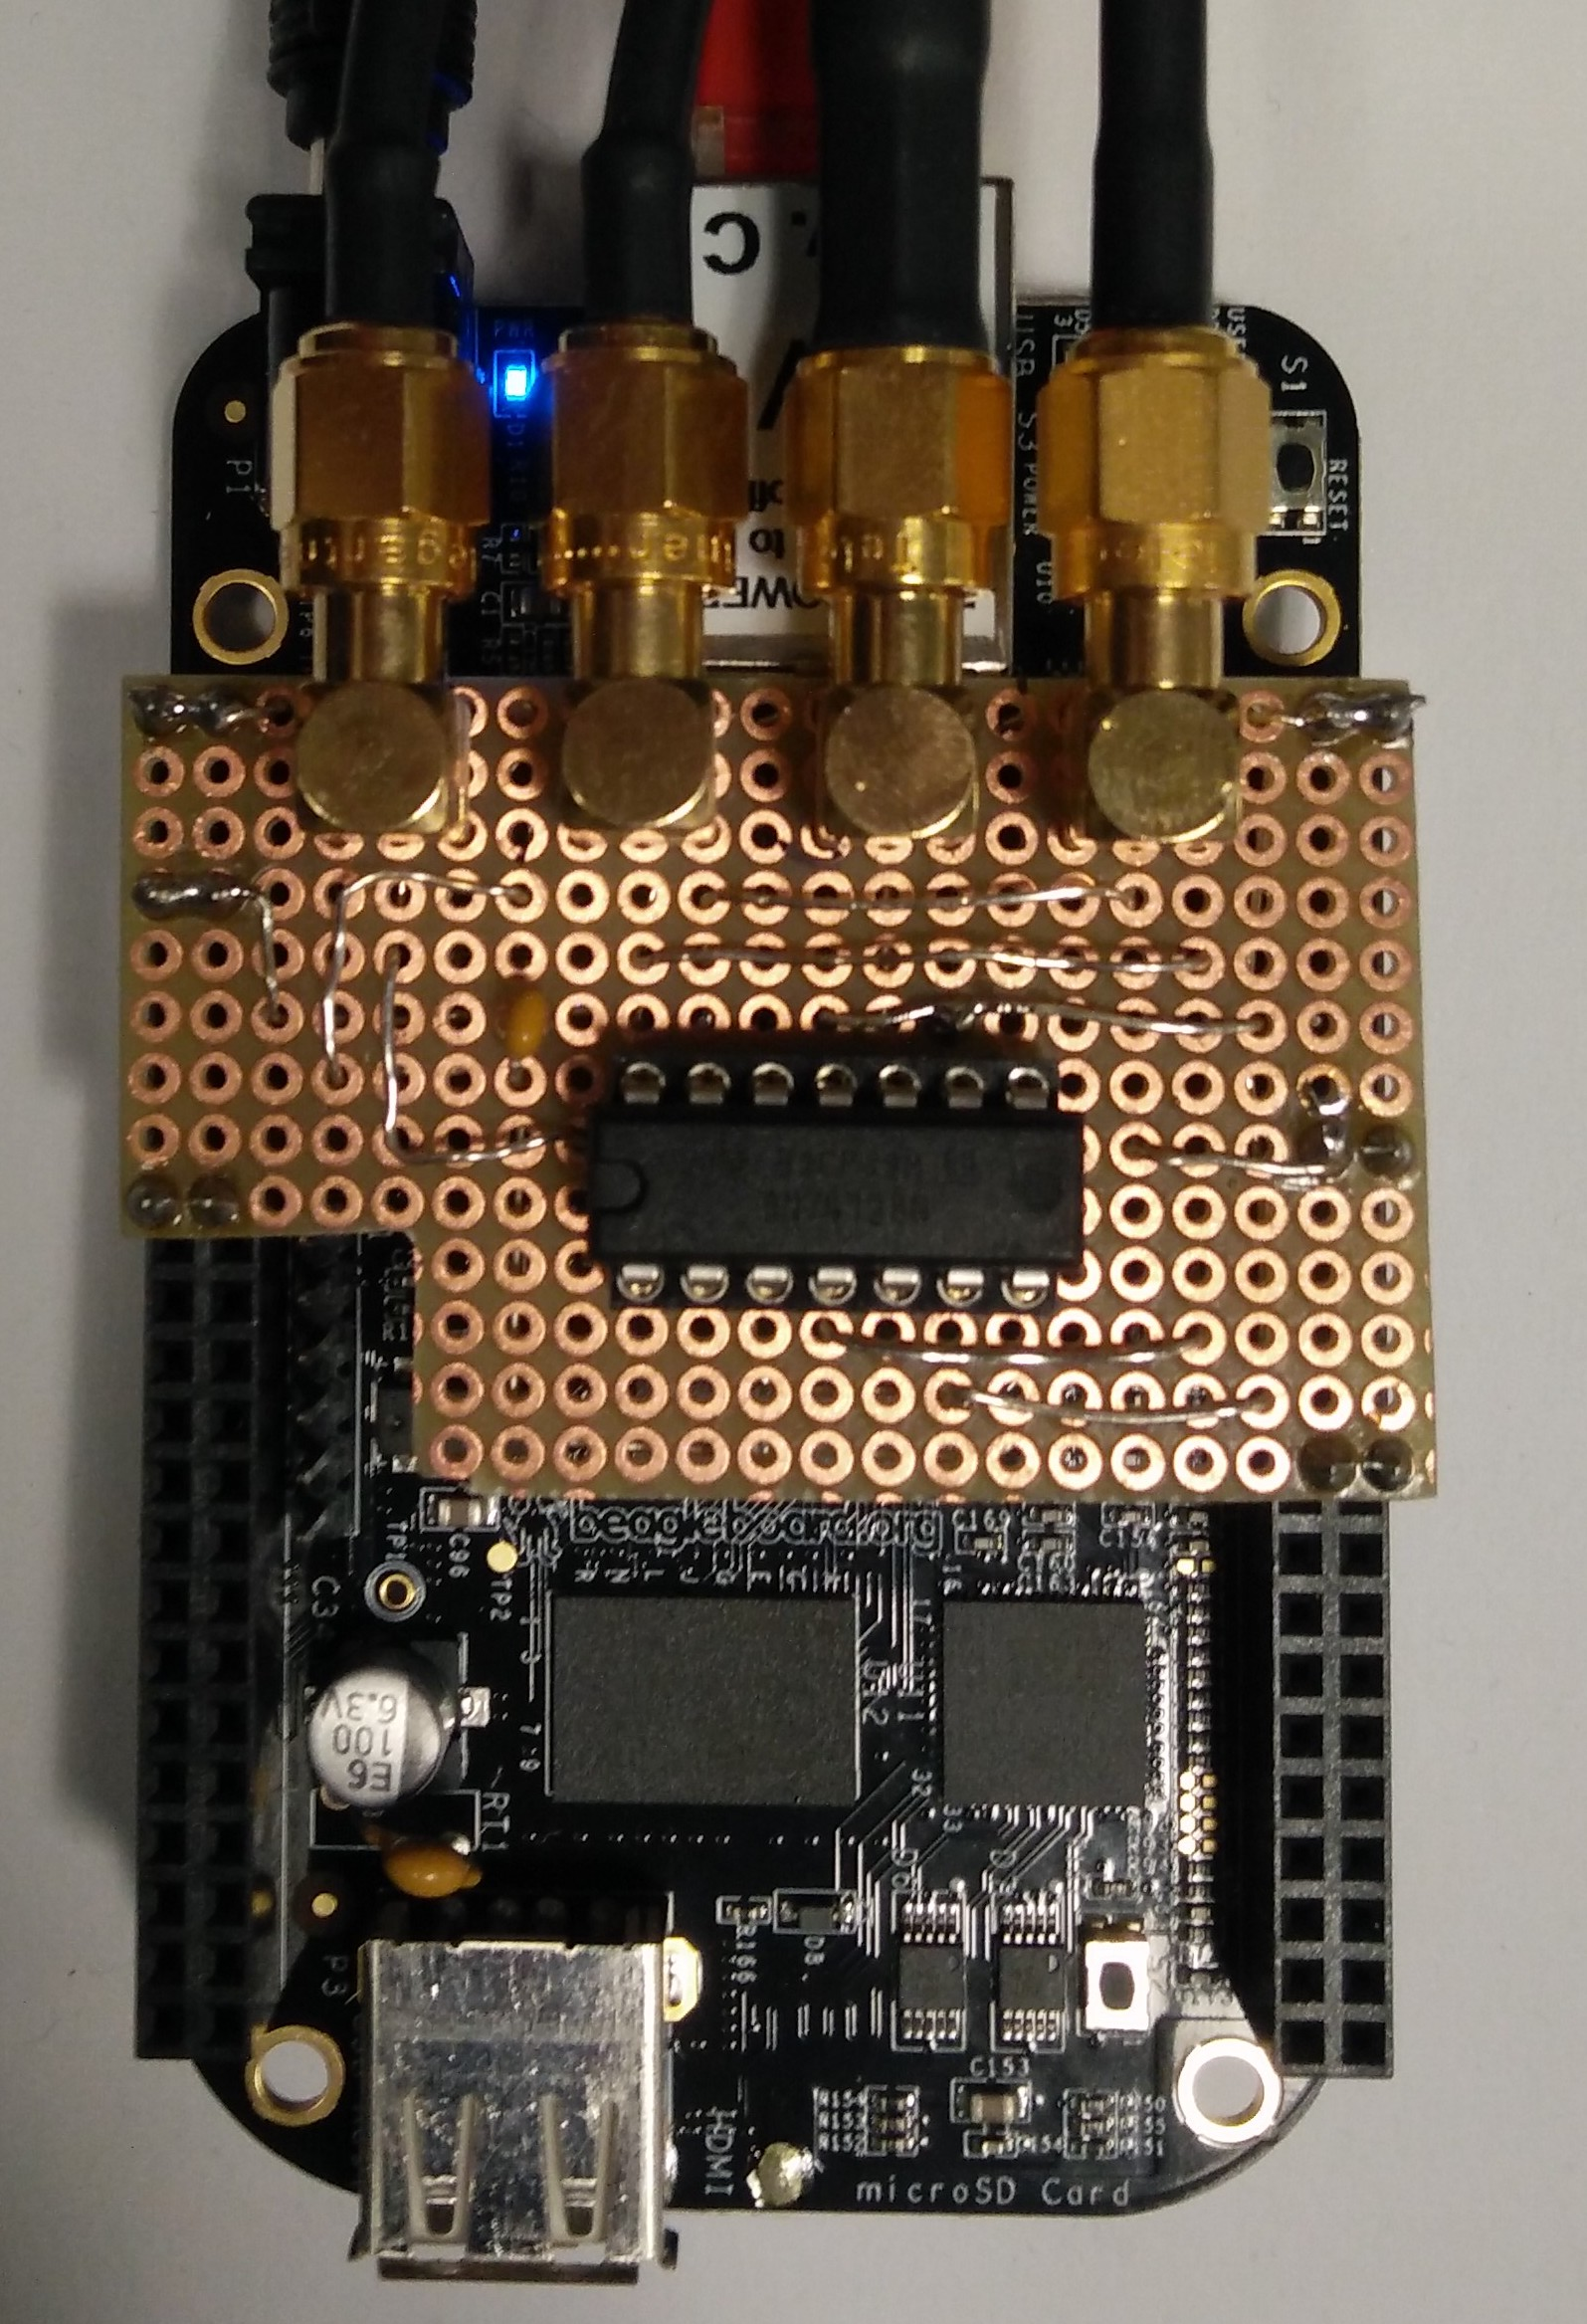
\includegraphics[width=.6\linewidth]{images/circuits/line-driver/board.jpg}
    \captionsetup{width=.8\linewidth}
    \caption{Picture of the trigger hub on the \gls{bbb}. The \gls{bbb} is
connected with the \gls{lan} via cable. The trigger hub forwards the signal
to the oscilloscope, the camera and the two \gls{dds}.}
  \end{minipage}
\end{figure}

\chapter{Calibration}

Alterations of the laboratory environment combined with the exchange of
components from the original setup made it advisable to recalibrate the setup.
In this chapter we want to document the steps necessary for calibration for
successive experiments.

\section{Fiber Coupling}

The visually shielded section of the setup used to reduce the output power
of the laser source is optically paired with the open section for beam
deflection via a \gls{smf} that only permits two orthogonal polarization and
a single gaussian mode. Through tuning the polarisator inside the power
reduction section we can try to match one of the orthogonal polarization
modes supported by the \gls{smf}. Polarization discrepancies induce the
polarization inside the \gls{smf} to oscillate on environmental changes like
temperature or vibration. Henceforth it is key to couple polarization modes
in order to ensure a stable operation.

The following receipt has proven to be successful to find an approximate
polarization match between the laser beam and the \gls{smf}. In addition
to the setup described in \cref{sec:powerbox} and \cref{sec:deflection}
an oscilloscope and a hot air gun are highly recommended.

\begin{enumerate}
  \item Connect the photodiode to the oscilloscope and use a coarse time
    scale of i.e. \SI{2}{\second}.
  \item Apply safety measures i.e. put on appropiete laser safety glasses and
    inform present personal of the imminent danger.
  \item Open the cover of the power reduction setup.
  \item Apply heat to the \gls{smf} through the hot air gun, alternatively
    you can try to move the fiber.
  \item The photodiode signal should start to oscillate. Tune the polarizor
    inside the power reduction subject to minimizing the oscillation.
\end{enumerate}

The oscillations occur as the polarization circulates inside the fiber and
will stop at some point. In this case yu should remove the heat or mechanical 
stress on the fiber and wait some time before you can reapply with the initial
response.

\section{Beam Alignment}

As is well known, beams that pass off-centered through spherical lenses
experience optical aberrations. Additionally we found that uncentered beams
may cause further optical defects from reflections at boundaries. Both effects
should be avoided as far as possible by adjusting positions and mirror angles.

As auxilliaries we recommend a pair of iris diaphragms that are mountable to
the lens mounts and a screen i.e. a white sheet of hard paper. With the iris
diaphragms we can easily find a center reference point visually by inspecting
the symmetry of the iris illumination at different pinhole diameters. Exact
steps are summarized in the below receipt. We refer to the optics as annotated
in \cref{fig:deflection}.

\begin{enumerate}
  \item Place screen in front of L2 and adjust screws on fiber coupler subject
    to a clean beam profile on the screen of the (1,1) diffraction order of
    the \gls{aom}s.
  \item Apply one iris to L2 and find center frequency of the \gls{aom}s.
  \item Mount irises on L3 and L4. Mount mirror pair M1, M2 to direct beam
    through both pinholes.
  \item Place auxilliary lens with mounted iris between L7 and M3 and adjust
    second objective pair L6, L7.
  \item Mount iris on L8 and place auxilliary lens with mounted iris in front
    of BS3. Align the mirror pair M3 and M4 to reflect the beam through both
    irises.
  \item Adjust the objective pair distance until you see an output similar to
    XY on the \gls{ccd} camera.
\end{enumerate}

The alignment of a mirror pair can be simplified by using the below algorithm:

\begin{enumerate}
  \item Select axis to align.
  \item Align the beam on the outside lens by tuning the inner mirror.
  \item Align the beam on the inner lens by tuning the outside mirror.
  \item Repeat steps 2 and 3 until beam is aligned on both lenses. Proceed
    with other axis.
\end{enumerate}

\section{Camera Focus}

Finally we had to reposition the camera to focus the incoming beam correctly
in order to register the beam profile as would be seen later by the atoms.
To find the precise focus position we followed the procedure described in
\cite{Hertlein2017} that consits of extracting the camera rail with its lens
and focusing it on a far distant object.

\begin{figure}[ht]
  \centering
  \includegraphics[width=\textwidth]{\builddir{focus.pdf}}
  \caption{Camera focused on far distant object. In this case a window from the
  building accross the courtyard.}
\end{figure}

\section{Beam Profile}

% Image from CCD camera with gaussian fit


\end{document}
